\documentclass[twoside]{book}

% Packages required by doxygen
\usepackage{fixltx2e}
\usepackage{calc}
\usepackage{doxygen}
\usepackage[export]{adjustbox} % also loads graphicx
\usepackage{graphicx}
\usepackage[utf8]{inputenc}
\usepackage{makeidx}
\usepackage{multicol}
\usepackage{multirow}
\PassOptionsToPackage{warn}{textcomp}
\usepackage{textcomp}
\usepackage[nointegrals]{wasysym}
\usepackage[table]{xcolor}

% Font selection
\usepackage[T1]{fontenc}
\usepackage[scaled=.90]{helvet}
\usepackage{courier}
\usepackage{amssymb}
\usepackage{sectsty}
\renewcommand{\familydefault}{\sfdefault}
\allsectionsfont{%
  \fontseries{bc}\selectfont%
  \color{darkgray}%
}
\renewcommand{\DoxyLabelFont}{%
  \fontseries{bc}\selectfont%
  \color{darkgray}%
}
\newcommand{\+}{\discretionary{\mbox{\scriptsize$\hookleftarrow$}}{}{}}

% Page & text layout
\usepackage{geometry}
\geometry{%
  a4paper,%
  top=2.5cm,%
  bottom=2.5cm,%
  left=2.5cm,%
  right=2.5cm%
}
\tolerance=750
\hfuzz=15pt
\hbadness=750
\setlength{\emergencystretch}{15pt}
\setlength{\parindent}{0cm}
\setlength{\parskip}{3ex plus 2ex minus 2ex}
\makeatletter
\renewcommand{\paragraph}{%
  \@startsection{paragraph}{4}{0ex}{-1.0ex}{1.0ex}{%
    \normalfont\normalsize\bfseries\SS@parafont%
  }%
}
\renewcommand{\subparagraph}{%
  \@startsection{subparagraph}{5}{0ex}{-1.0ex}{1.0ex}{%
    \normalfont\normalsize\bfseries\SS@subparafont%
  }%
}
\makeatother

% Headers & footers
\usepackage{fancyhdr}
\pagestyle{fancyplain}
\fancyhead[LE]{\fancyplain{}{\bfseries\thepage}}
\fancyhead[CE]{\fancyplain{}{}}
\fancyhead[RE]{\fancyplain{}{\bfseries\leftmark}}
\fancyhead[LO]{\fancyplain{}{\bfseries\rightmark}}
\fancyhead[CO]{\fancyplain{}{}}
\fancyhead[RO]{\fancyplain{}{\bfseries\thepage}}
\fancyfoot[LE]{\fancyplain{}{}}
\fancyfoot[CE]{\fancyplain{}{}}
\fancyfoot[RE]{\fancyplain{}{\bfseries\scriptsize Generated by Doxygen }}
\fancyfoot[LO]{\fancyplain{}{\bfseries\scriptsize Generated by Doxygen }}
\fancyfoot[CO]{\fancyplain{}{}}
\fancyfoot[RO]{\fancyplain{}{}}
\renewcommand{\footrulewidth}{0.4pt}
\renewcommand{\chaptermark}[1]{%
  \markboth{#1}{}%
}
\renewcommand{\sectionmark}[1]{%
  \markright{\thesection\ #1}%
}

% Indices & bibliography
\usepackage{natbib}
\usepackage[titles]{tocloft}
\setcounter{tocdepth}{3}
\setcounter{secnumdepth}{5}
\makeindex

% Hyperlinks (required, but should be loaded last)
\usepackage{ifpdf}
\ifpdf
  \usepackage[pdftex,pagebackref=true]{hyperref}
\else
  \usepackage[ps2pdf,pagebackref=true]{hyperref}
\fi
\hypersetup{%
  colorlinks=true,%
  linkcolor=blue,%
  citecolor=blue,%
  unicode%
}

% Custom commands
\newcommand{\clearemptydoublepage}{%
  \newpage{\pagestyle{empty}\cleardoublepage}%
}

\usepackage{caption}
\captionsetup{labelsep=space,justification=centering,font={bf},singlelinecheck=off,skip=4pt,position=top}

%===== C O N T E N T S =====

\begin{document}

% Titlepage & ToC
\hypersetup{pageanchor=false,
             bookmarksnumbered=true,
             pdfencoding=unicode
            }
\pagenumbering{alph}
\begin{titlepage}
\vspace*{7cm}
\begin{center}%
{\Large My Project }\\
\vspace*{1cm}
{\large Generated by Doxygen 1.8.14}\\
\end{center}
\end{titlepage}
\clearemptydoublepage
\pagenumbering{roman}
\tableofcontents
\clearemptydoublepage
\pagenumbering{arabic}
\hypersetup{pageanchor=true}

%--- Begin generated contents ---
\chapter{D\+A\+Com P\+R\+O\+T\+O\+C\+OL}
\label{md__r_e_a_d_m_e}
\Hypertarget{md__r_e_a_d_m_e}
\subsection*{The economic model of an alternative society}

The rules are simple. Game objective are the money themselves. You can get in with any amount and on the next day you get more or less than starting amount. You can loose max. 30\%, but if you win, you starting amonut can be multiplied by many times. Interesting feature is that you can get your money anytime you want.


\begin{DoxyItemize}
\item The Protocol offers F\+R\+E\+E\+D\+OM to people.
\item Money -\/ the subject of the Protocol.
\item Capital growth 10-\/1000+\% per month.
\item Automated redistributing system of money, where everyone wins.
\item Mass use. Suggest your friends to sponsor your trip, and gain on it immediately.
\item Fixed percent of loss. Maximum loss is always specified.
\item The Protocol is based on a unique double-\/rate algorithm with overlapping and self-\/quotation.
\item Absolute financial balance. The Protocol is N\+OT a financial pyramid.
\item The game is played by Rounds. Lost in one round -\/ you win back in another.
\item Absolute decentralization. Works on E\+OS operating system.
\item Open source code.
\item Economic mixer. Increases the G\+DP of any country by speeding up financial flows.
\item The Way to the New Age. The Golden Century will come with the everywhere use of the Protocol.
\end{DoxyItemize}

\section*{How it works}

Figuratively, the Protocol can be represented as a rotating Spiral. There is a game fund in the middle of the Spiral, which always has its color -\/ black or white. Completing the turn, the Spiral switches the color of the fund. When the new color of the fund matches with yours -\/ you win, when not -\/ lose. Money can be collected at any time.

 

The twisting movement of the Spiral is given by players, the power of spin and the lasting of the game depend on them. The vertical growth of the Spiral is the increase of benefit, it is set up by the mathematical algorithm. The more turns passed to the stop -\/ the more profitability.

When the rotation stop, all participants receive winnings and losses according to the current selling rates for the winners, and a fixed number of decrease for the loses. Each new tern of the Spiral is called a Round.

 

\section*{How to play}

In the account you will find the control panel. When you select the Participation Protocol branch, you change the gain of winnings with each new round and a fixed percentage of losses. Where there are more losses, the winnings are sweeter.

By clicking on the Deposit button, you enter the game and get the color -\/ the same as the color of the current Round. In order to win, the Round must switch to the next color, and then again -\/ to your. There are no restrictions for the number of deposits; you can have several balances of opposite colors at the same time.

You can withdraw money at any time. If you exit the game on the same round as you entered -\/ you do not lose anything. If on the opposite color -\/ you lose the set percentage of the entry amount. If on your following color -\/ you win according to the prediction defined in advance.

Sooner or later, the extention of the round slows down and stops -\/ and no one knows exactly when it will happen. If the round does not close within the agreed time, for example, for 3 days, then a new cycle of the branch of the Protocol starts -\/ all players get their winnings and losses according to the last color of the round and enter the game anew if they wish. The rules and conditions for the new cycle are saved.

\section*{It is N\+OT a pyramid}

Anyone can check all the algorithms and financial balances of the Protocol, as the code and all the tables are always open. No one can change them, no one can intervene and take the \char`\"{}box\char`\"{} with money, no one can stop the growth of the Protocol.

Since the Protocol is based on a mathematical algorithm and always has a positive financial balance enough to pay 100\% to participants according to established rules, any reproaches about the involvement of the Protocol in the use of the Ponzi scheme can be prosecuted in private, as they do not have no reason.

\section*{Business model for companies and active participants}

Each participant can become an organizer of a branch of the Protocol. The original parameters to any goals and objectives\+It may be regulated, whether it is the speed-\/up of family financial flows, the welfare of a religious sect or the flight to Mars. Just Suggest your friends to sponsor your trip, and gain on it, and probably you will get it already tomorrow.

The Protocol can work for any number of participants and starting capital. It can be considered as a model of collective financing of any engagement, where the participants immediately receive profit, and the organizer -\/ the financial flow for the realization of the dream. 
\chapter{Hierarchical Index}
\section{Class Hierarchy}
This inheritance list is sorted roughly, but not completely, alphabetically\+:\begin{DoxyCompactList}
\item \contentsline{section}{ahosts}{\pageref{structahosts}}{}
\item \contentsline{section}{badges}{\pageref{structbadges}}{}
\item \contentsline{section}{balance}{\pageref{structbalance}}{}
\item \contentsline{section}{benefactors}{\pageref{structbenefactors}}{}
\item \contentsline{section}{bwtradegraph}{\pageref{structbwtradegraph}}{}
\item \contentsline{section}{cmsconfig}{\pageref{structcmsconfig}}{}
\item \contentsline{section}{cmscontent}{\pageref{structcmscontent}}{}
\item \contentsline{section}{conditions}{\pageref{structconditions}}{}
\item \contentsline{section}{market\+:\+:connector}{\pageref{structmarket_1_1connector}}{}
\item contract\begin{DoxyCompactList}
\item \contentsline{section}{eosio\+:\+:token}{\pageref{classeosio_1_1token}}{}
\item \contentsline{section}{unicore}{\pageref{classunicore}}{}
\end{DoxyCompactList}
\item \contentsline{section}{coredhistory}{\pageref{structcoredhistory}}{}
\item \contentsline{section}{cpartners}{\pageref{structcpartners}}{}
\item \contentsline{section}{currency\+\_\+stats}{\pageref{structcurrency__stats}}{}
\item \contentsline{section}{cycle}{\pageref{structcycle}}{}
\item \contentsline{section}{cycle3}{\pageref{structcycle3}}{}
\item \contentsline{section}{dacs}{\pageref{structdacs}}{}
\item \contentsline{section}{debts}{\pageref{structdebts}}{}
\item \contentsline{section}{delegations}{\pageref{structdelegations}}{}
\item \contentsline{section}{dlog}{\pageref{structdlog}}{}
\item \contentsline{section}{emission}{\pageref{structemission}}{}
\item \contentsline{section}{funds}{\pageref{structfunds}}{}
\item \contentsline{section}{goals}{\pageref{structgoals}}{}
\item \contentsline{section}{goalspartic}{\pageref{structgoalspartic}}{}
\item \contentsline{section}{gpercents}{\pageref{structgpercents}}{}
\item \contentsline{section}{hosts}{\pageref{structhosts}}{}
\item \contentsline{section}{hostsonfunds}{\pageref{structhostsonfunds}}{}
\item \contentsline{section}{market}{\pageref{structmarket}}{}
\item \contentsline{section}{partners}{\pageref{structpartners}}{}
\item \contentsline{section}{plog}{\pageref{structplog}}{}
\item \contentsline{section}{pool}{\pageref{structpool}}{}
\item \contentsline{section}{power}{\pageref{structpower}}{}
\item \contentsline{section}{pstats}{\pageref{structpstats}}{}
\item \contentsline{section}{rate}{\pageref{structrate}}{}
\item \contentsline{section}{refbalances}{\pageref{structrefbalances}}{}
\item \contentsline{section}{reports}{\pageref{structreports}}{}
\item \contentsline{section}{roles}{\pageref{structroles}}{}
\item \contentsline{section}{rstat}{\pageref{structrstat}}{}
\item \contentsline{section}{sale}{\pageref{structsale}}{}
\item \contentsline{section}{sincome}{\pageref{structsincome}}{}
\item \contentsline{section}{spiral}{\pageref{structspiral}}{}
\item \contentsline{section}{tasks}{\pageref{structtasks}}{}
\item \contentsline{section}{usbadges}{\pageref{structusbadges}}{}
\item \contentsline{section}{userscount}{\pageref{structuserscount}}{}
\item \contentsline{section}{vesting}{\pageref{structvesting}}{}
\item \contentsline{section}{votes}{\pageref{structvotes}}{}
\end{DoxyCompactList}

\chapter{Class Index}
\section{Class List}
Here are the classes, structs, unions and interfaces with brief descriptions\+:\begin{DoxyCompactList}
\item\contentsline{section}{\mbox{\hyperlink{structahosts}{ahosts}} \\*Структура хостов, платформ и их сайтов }{\pageref{structahosts}}{}
\item\contentsline{section}{\mbox{\hyperlink{structbadges}{badges}} \\*Структура наградных значков хоста Двойной Спирали, их изображений, пиктограмм и предоставляемой силы }{\pageref{structbadges}}{}
\item\contentsline{section}{\mbox{\hyperlink{structbalance}{balance}} \\*Структура балансов пользователя у всех хостов Двойной Спирали }{\pageref{structbalance}}{}
\item\contentsline{section}{\mbox{\hyperlink{structbenefactors}{benefactors}} \\*Структура бенефакторов цели хоста Двойной Спирали }{\pageref{structbenefactors}}{}
\item\contentsline{section}{\mbox{\hyperlink{structbwtradegraph}{bwtradegraph}} \\*Структура для отображения Двойной Спирали в виде торгового графика типа B\+L\+A\+C\+K-\/\+A\+N\+D-\/\+W\+H\+I\+TE }{\pageref{structbwtradegraph}}{}
\item\contentsline{section}{\mbox{\hyperlink{structcmsconfig}{cmsconfig}} \\*Структура конфигурации платформы }{\pageref{structcmsconfig}}{}
\item\contentsline{section}{\mbox{\hyperlink{structcmscontent}{cmscontent}} \\*Структура хранилища контента и оформления платформ }{\pageref{structcmscontent}}{}
\item\contentsline{section}{\mbox{\hyperlink{structconditions}{conditions}} \\*Структура хранилища универсального набора условий, относящихся к хосту, платформе или протоколу }{\pageref{structconditions}}{}
\item\contentsline{section}{\mbox{\hyperlink{structmarket_1_1connector}{market\+::connector}} \\*Структура коннектора рынка торгового робота Bancor }{\pageref{structmarket_1_1connector}}{}
\item\contentsline{section}{\mbox{\hyperlink{structexchange__state_1_1connector}{exchange\+\_\+state\+::connector}} }{\pageref{structexchange__state_1_1connector}}{}
\item\contentsline{section}{\mbox{\hyperlink{structcoredhistory}{coredhistory}} \\*Структура для хранения сообщений в режиме чата ограниченной длинны от спонсоров хоста Двойной Спирали }{\pageref{structcoredhistory}}{}
\item\contentsline{section}{\mbox{\hyperlink{structcpartners2}{cpartners2}} \\*Структура учёта партнёров и их статусов у хоста Двойной Спирали }{\pageref{structcpartners2}}{}
\item\contentsline{section}{\mbox{\hyperlink{structcurrency__stats}{currency\+\_\+stats}} \\*Структура статистики жетонов в обороте }{\pageref{structcurrency__stats}}{}
\item\contentsline{section}{\mbox{\hyperlink{structcycle}{cycle}} \\*Структура для учёта развития циклов хоста Двойной Спирали }{\pageref{structcycle}}{}
\item\contentsline{section}{\mbox{\hyperlink{structcycle3}{cycle3}} \\*Структура для учёта сжигания внутренней конвертационной единицы }{\pageref{structcycle3}}{}
\item\contentsline{section}{\mbox{\hyperlink{structdacs}{dacs}} \\*Структура команды хоста Двойной Спирали }{\pageref{structdacs}}{}
\item\contentsline{section}{\mbox{\hyperlink{structdebts}{debts}} \\*Структура целевого долга хоста Двойной Спирали }{\pageref{structdebts}}{}
\item\contentsline{section}{\mbox{\hyperlink{structdelegations}{delegations}} \\*Структура учёта делегированной силы от пользователя к пользователю }{\pageref{structdelegations}}{}
\item\contentsline{section}{\mbox{\hyperlink{structdlog}{dlog}} \\*Структура истории получения безусловного потока жетонов пользователем у хоста Двойной Спирали }{\pageref{structdlog}}{}
\item\contentsline{section}{\mbox{\hyperlink{structdoers}{doers}} \\*Структура деятелей по задаче }{\pageref{structdoers}}{}
\item\contentsline{section}{\mbox{\hyperlink{structemission}{emission}} \\*Структура параметров эмиссии целевого фонда хоста Двойной Спирали }{\pageref{structemission}}{}
\item\contentsline{section}{\mbox{\hyperlink{structexchange__state}{exchange\+\_\+state}} }{\pageref{structexchange__state}}{}
\item\contentsline{section}{\mbox{\hyperlink{structfunds}{funds}} \\*Структура глобальных фондов владельцев жетонов, помещенных на распределение }{\pageref{structfunds}}{}
\item\contentsline{section}{\mbox{\hyperlink{structgoals}{goals}} \\*Структура целей хоста Двойной Спирали }{\pageref{structgoals}}{}
\item\contentsline{section}{\mbox{\hyperlink{structgoals3}{goals3}} \\*Структура целей хоста Двойной Спирали }{\pageref{structgoals3}}{}
\item\contentsline{section}{\mbox{\hyperlink{structgoalspartic}{goalspartic}} \\*Структура участников цели хоста Двойной Спирали }{\pageref{structgoalspartic}}{}
\item\contentsline{section}{\mbox{\hyperlink{structgpercents}{gpercents}} \\*Структура системного процента, изымаего протокол из обращения при каждом полу-\/обороте Двойной Спирали каждого хоста }{\pageref{structgpercents}}{}
\item\contentsline{section}{\mbox{\hyperlink{structguests}{guests}} }{\pageref{structguests}}{}
\item\contentsline{section}{\mbox{\hyperlink{structhosts}{hosts}} \\*Структура хоста Двойной Спирали }{\pageref{structhosts}}{}
\item\contentsline{section}{\mbox{\hyperlink{structhosts2}{hosts2}} \\*Расширение структуры хоста Двойной Спирали }{\pageref{structhosts2}}{}
\item\contentsline{section}{\mbox{\hyperlink{structhostsonfunds}{hostsonfunds}} \\*Структура хостов Двойной Спирали, подключенных к глобальным фондам распределения }{\pageref{structhostsonfunds}}{}
\item\contentsline{section}{\mbox{\hyperlink{structincoming}{incoming}} \\*Структура задач, где аккаунт деятель }{\pageref{structincoming}}{}
\item\contentsline{section}{\mbox{\hyperlink{structmarket}{market}} \\*Структура взамодействия с рынками торгового робота Bancor }{\pageref{structmarket}}{}
\item\contentsline{section}{\mbox{\hyperlink{structpartners2}{partners2}} \\*Структура партнёров и их партнёров }{\pageref{structpartners2}}{}
\item\contentsline{section}{\mbox{\hyperlink{structplog}{plog}} \\*Структура истории преобретения силы пользователем у хоста Двойной Спирали }{\pageref{structplog}}{}
\item\contentsline{section}{\mbox{\hyperlink{structpool}{pool}} \\*Структура для учёта распределения бассейнов внутренней учетной единицы хоста Двойной Спирали }{\pageref{structpool}}{}
\item\contentsline{section}{\mbox{\hyperlink{structpower}{power}} \\*Структура силы пользователя у хоста Двойной Спирали }{\pageref{structpower}}{}
\item\contentsline{section}{\mbox{\hyperlink{structpower2}{power2}} \\*Расширение структуры силы пользователя у хоста Двойной Спирали }{\pageref{structpower2}}{}
\item\contentsline{section}{\mbox{\hyperlink{structpower3}{power3}} \\*Обновленная структура силы пользователя у хоста Двойной Спирали }{\pageref{structpower3}}{}
\item\contentsline{section}{\mbox{\hyperlink{structproducer__info}{producer\+\_\+info}} }{\pageref{structproducer__info}}{}
\item\contentsline{section}{\mbox{\hyperlink{structpstats}{pstats}} \\*Структура статистики распределения безусловного потока жетонов хоста Двойной Спирали }{\pageref{structpstats}}{}
\item\contentsline{section}{\mbox{\hyperlink{structrate}{rate}} \\*Структура курсов реализации внутренней конвертационной единицы и их возврата Протоколу }{\pageref{structrate}}{}
\item\contentsline{section}{\mbox{\hyperlink{structrefbalances}{refbalances}} \\*Структура полученных реферальных балансов от партнёров на партнёра }{\pageref{structrefbalances}}{}
\item\contentsline{section}{\mbox{\hyperlink{structreports3}{reports3}} \\*Структура отчетов по задачам хоста Двойной Спирали }{\pageref{structreports3}}{}
\item\contentsline{section}{\mbox{\hyperlink{structroles}{roles}} \\*Структура командных ролей протокола }{\pageref{structroles}}{}
\item\contentsline{section}{\mbox{\hyperlink{structrstat}{rstat}} \\*Структура статистики реферальных балансов и осадок, доступный на получение по мере накопления }{\pageref{structrstat}}{}
\item\contentsline{section}{\mbox{\hyperlink{structrvotes}{rvotes}} \\*Структура голосов за отчёты }{\pageref{structrvotes}}{}
\item\contentsline{section}{\mbox{\hyperlink{structsale}{sale}} \\*Структура истории движения жетона распределения хоста Двойной Спирали }{\pageref{structsale}}{}
\item\contentsline{section}{\mbox{\hyperlink{structsincome}{sincome}} \\*Структура учёта системного дохода фондов хоста Двойной Спирали }{\pageref{structsincome}}{}
\item\contentsline{section}{\mbox{\hyperlink{structsincome2}{sincome2}} \\*Доп структура учёта системного дохода фондов хоста Двойной Спирали }{\pageref{structsincome2}}{}
\item\contentsline{section}{\mbox{\hyperlink{structspiral}{spiral}} \\*Структура основных параметров конфигурации Двойной Спирали }{\pageref{structspiral}}{}
\item\contentsline{section}{\mbox{\hyperlink{structspiral2}{spiral2}} \\*Структура компенсационных параметров конфигурации Двойной Спирали }{\pageref{structspiral2}}{}
\item\contentsline{section}{\mbox{\hyperlink{structtasks}{tasks}} \\*Структура задач хоста Двойной Спирали }{\pageref{structtasks}}{}
\item\contentsline{section}{\mbox{\hyperlink{classeosio_1_1token}{eosio\+::token}} \\*Класс взаимодействия с жетонами операционной системы }{\pageref{classeosio_1_1token}}{}
\item\contentsline{section}{\mbox{\hyperlink{classunicore}{unicore}} \\*Содержит все доступные действия, публичные и приватные методы протокола }{\pageref{classunicore}}{}
\item\contentsline{section}{\mbox{\hyperlink{structusbadges}{usbadges}} \\*Структура наградных значков пользователя, полученных от разных хостов Двойной Спирали }{\pageref{structusbadges}}{}
\item\contentsline{section}{\mbox{\hyperlink{structuserscount}{userscount}} \\*Структура статистики количества зарегистрированных пользователей }{\pageref{structuserscount}}{}
\item\contentsline{section}{\mbox{\hyperlink{structvacs}{vacs}} \\*Структура вакансии хоста Двойной Спирали }{\pageref{structvacs}}{}
\item\contentsline{section}{\mbox{\hyperlink{structvesting}{vesting}} \\*Структура учёта вестинг-\/балансов пользователей при возврате силы хосту Двойной Спирали }{\pageref{structvesting}}{}
\item\contentsline{section}{\mbox{\hyperlink{structvotes}{votes}} \\*Структура голосов за цели хоста Двойной Спирали }{\pageref{structvotes}}{}
\item\contentsline{section}{\mbox{\hyperlink{structvproposal}{vproposal}} \\*Структура заявки на вакансию хоста Двойной Спирали }{\pageref{structvproposal}}{}
\end{DoxyCompactList}

\chapter{File Index}
\section{File List}
Here is a list of all documented files with brief descriptions\+:\begin{DoxyCompactList}
\item\contentsline{section}{{\bfseries badges.\+hpp} }{\pageref{badges_8hpp}}{}
\item\contentsline{section}{{\bfseries binary.\+hpp} }{\pageref{binary_8hpp}}{}
\item\contentsline{section}{{\bfseries cms.\+hpp} }{\pageref{cms_8hpp}}{}
\item\contentsline{section}{\mbox{\hyperlink{eosio_8token_8hpp}{eosio.\+token.\+hpp}} }{\pageref{eosio_8token_8hpp}}{}
\item\contentsline{section}{{\bfseries exchange\+\_\+state.\+hpp} }{\pageref{exchange__state_8hpp}}{}
\item\contentsline{section}{{\bfseries goals.\+hpp} }{\pageref{goals_8hpp}}{}
\item\contentsline{section}{{\bfseries hosts.\+hpp} }{\pageref{hosts_8hpp}}{}
\item\contentsline{section}{{\bfseries ipfs.\+hpp} }{\pageref{ipfs_8hpp}}{}
\item\contentsline{section}{{\bfseries protocol.\+hpp} }{\pageref{protocol_8hpp}}{}
\item\contentsline{section}{{\bfseries shares.\+hpp} }{\pageref{shares_8hpp}}{}
\item\contentsline{section}{{\bfseries tasks.\+hpp} }{\pageref{tasks_8hpp}}{}
\item\contentsline{section}{{\bfseries voting.\+hpp} }{\pageref{voting_8hpp}}{}
\end{DoxyCompactList}

\chapter{Class Documentation}
\hypertarget{structeosio_1_1approver}{}\section{eosio\+:\+:approver Struct Reference}
\label{structeosio_1_1approver}\index{eosio\+::approver@{eosio\+::approver}}
\subsection*{Public Attributes}
\begin{DoxyCompactItemize}
\item 
\mbox{\Hypertarget{structeosio_1_1approver_a0fd071d070b256daaa175ea523c43386}\label{structeosio_1_1approver_a0fd071d070b256daaa175ea523c43386}} 
account\+\_\+name {\bfseries host}
\item 
\mbox{\Hypertarget{structeosio_1_1approver_aea3e203759357b81546cae94f6c1047f}\label{structeosio_1_1approver_aea3e203759357b81546cae94f6c1047f}} 
uint64\+\_\+t {\bfseries report\+\_\+id}
\item 
\mbox{\Hypertarget{structeosio_1_1approver_ab7abb3428b9df1385b0216b5f6fdc1ee}\label{structeosio_1_1approver_ab7abb3428b9df1385b0216b5f6fdc1ee}} 
eosio\+::string {\bfseries comment}
\end{DoxyCompactItemize}


The documentation for this struct was generated from the following file\+:\begin{DoxyCompactItemize}
\item 
tasks.\+hpp\end{DoxyCompactItemize}

\hypertarget{structeosio_1_1backbadge}{}\section{eosio\+:\+:backbadge Struct Reference}
\label{structeosio_1_1backbadge}\index{eosio\+::backbadge@{eosio\+::backbadge}}
\subsection*{Public Attributes}
\begin{DoxyCompactItemize}
\item 
\mbox{\Hypertarget{structeosio_1_1backbadge_a99dcddf14a170cac1f849d28b71d4f76}\label{structeosio_1_1backbadge_a99dcddf14a170cac1f849d28b71d4f76}} 
account\+\_\+name {\bfseries host}
\item 
\mbox{\Hypertarget{structeosio_1_1backbadge_afacb89cce1f3323007ed6a4e60ccdd19}\label{structeosio_1_1backbadge_afacb89cce1f3323007ed6a4e60ccdd19}} 
account\+\_\+name {\bfseries from}
\item 
\mbox{\Hypertarget{structeosio_1_1backbadge_abd90ebcbd4af636b220dff0d38cb5ee6}\label{structeosio_1_1backbadge_abd90ebcbd4af636b220dff0d38cb5ee6}} 
uint64\+\_\+t {\bfseries badge\+\_\+id}
\item 
\mbox{\Hypertarget{structeosio_1_1backbadge_ad911838ee3124447394ac853646256d8}\label{structeosio_1_1backbadge_ad911838ee3124447394ac853646256d8}} 
eosio\+::string {\bfseries comment}
\end{DoxyCompactItemize}


The documentation for this struct was generated from the following file\+:\begin{DoxyCompactItemize}
\item 
badges.\+hpp\end{DoxyCompactItemize}

\hypertarget{structbadge__struct}{}\section{badge\+\_\+struct Struct Reference}
\label{structbadge__struct}\index{badge\+\_\+struct@{badge\+\_\+struct}}
\subsection*{Public Member Functions}
\begin{DoxyCompactItemize}
\item 
\mbox{\Hypertarget{structbadge__struct_a66403d83fdc587d59b4124b65733ff4e}\label{structbadge__struct_a66403d83fdc587d59b4124b65733ff4e}} 
void {\bfseries setbadge\+\_\+action} (const \mbox{\hyperlink{structeosio_1_1setbadge}{setbadge}} \&op)
\item 
\mbox{\Hypertarget{structbadge__struct_ab013e63941cf00e26f9d208f84fc5c71}\label{structbadge__struct_ab013e63941cf00e26f9d208f84fc5c71}} 
void {\bfseries giftbadge\+\_\+action} (const \mbox{\hyperlink{structeosio_1_1giftbadge}{giftbadge}} \&op)
\item 
\mbox{\Hypertarget{structbadge__struct_a3b12637b107f7c10e0dc2956fec04c02}\label{structbadge__struct_a3b12637b107f7c10e0dc2956fec04c02}} 
void {\bfseries backbadge\+\_\+action} (const \mbox{\hyperlink{structeosio_1_1backbadge}{backbadge}} \&op)
\end{DoxyCompactItemize}


The documentation for this struct was generated from the following file\+:\begin{DoxyCompactItemize}
\item 
badges.\+cpp\end{DoxyCompactItemize}

\hypertarget{structeosio_1_1badges}{}\section{eosio\+:\+:badges Struct Reference}
\label{structeosio_1_1badges}\index{eosio\+::badges@{eosio\+::badges}}
\subsection*{Public Member Functions}
\begin{DoxyCompactItemize}
\item 
\mbox{\Hypertarget{structeosio_1_1badges_a4ce3a0e92e27d9ff173990df5762eb60}\label{structeosio_1_1badges_a4ce3a0e92e27d9ff173990df5762eb60}} 
uint64\+\_\+t {\bfseries primary\+\_\+key} () const
\end{DoxyCompactItemize}
\subsection*{Public Attributes}
\begin{DoxyCompactItemize}
\item 
\mbox{\Hypertarget{structeosio_1_1badges_a89b3ce5ce0f480c3f811c0e6ae31aac8}\label{structeosio_1_1badges_a89b3ce5ce0f480c3f811c0e6ae31aac8}} 
uint64\+\_\+t {\bfseries id}
\item 
\mbox{\Hypertarget{structeosio_1_1badges_a891b1c8798996eeaebfb0ee962e48e72}\label{structeosio_1_1badges_a891b1c8798996eeaebfb0ee962e48e72}} 
eosio\+::string {\bfseries caption}
\item 
\mbox{\Hypertarget{structeosio_1_1badges_a5660dc2a36d1aafe0fe11e976b264e9c}\label{structeosio_1_1badges_a5660dc2a36d1aafe0fe11e976b264e9c}} 
eosio\+::string {\bfseries description}
\item 
\mbox{\Hypertarget{structeosio_1_1badges_a7338d05cac1d40b12a31a372252e4be2}\label{structeosio_1_1badges_a7338d05cac1d40b12a31a372252e4be2}} 
eosio\+::string {\bfseries iurl}
\item 
\mbox{\Hypertarget{structeosio_1_1badges_ade9193e2fd897844f2ec2297c33c5056}\label{structeosio_1_1badges_ade9193e2fd897844f2ec2297c33c5056}} 
uint64\+\_\+t {\bfseries total}
\item 
\mbox{\Hypertarget{structeosio_1_1badges_a434cacbcfcac81b18ae18183dcd1d366}\label{structeosio_1_1badges_a434cacbcfcac81b18ae18183dcd1d366}} 
uint64\+\_\+t {\bfseries remain}
\item 
\mbox{\Hypertarget{structeosio_1_1badges_a5a5b41dae3374fde91b1f0fc8b3d5af8}\label{structeosio_1_1badges_a5a5b41dae3374fde91b1f0fc8b3d5af8}} 
uint64\+\_\+t {\bfseries power}
\end{DoxyCompactItemize}


The documentation for this struct was generated from the following file\+:\begin{DoxyCompactItemize}
\item 
badges.\+hpp\end{DoxyCompactItemize}

\hypertarget{structeosio_1_1balance}{}\section{eosio\+:\+:balance Struct Reference}
\label{structeosio_1_1balance}\index{eosio\+::balance@{eosio\+::balance}}
\subsection*{Public Member Functions}
\begin{DoxyCompactItemize}
\item 
\mbox{\Hypertarget{structeosio_1_1balance_a61bf7990c26d6f28f6507e1fd2c56e44}\label{structeosio_1_1balance_a61bf7990c26d6f28f6507e1fd2c56e44}} 
uint64\+\_\+t {\bfseries primary\+\_\+key} () const
\end{DoxyCompactItemize}
\subsection*{Public Attributes}
\begin{DoxyCompactItemize}
\item 
\mbox{\Hypertarget{structeosio_1_1balance_a4108c954aff6120398b436af885ee1e5}\label{structeosio_1_1balance_a4108c954aff6120398b436af885ee1e5}} 
uint64\+\_\+t {\bfseries id}
\item 
\mbox{\Hypertarget{structeosio_1_1balance_a3d9257d714d1d39e3770d5aeda4d9f90}\label{structeosio_1_1balance_a3d9257d714d1d39e3770d5aeda4d9f90}} 
eosio\+::name {\bfseries host}
\item 
\mbox{\Hypertarget{structeosio_1_1balance_a4c1cbc34dd3a23e3c6b4a70dbffe6f48}\label{structeosio_1_1balance_a4c1cbc34dd3a23e3c6b4a70dbffe6f48}} 
eosio\+::name {\bfseries chost}
\item 
\mbox{\Hypertarget{structeosio_1_1balance_a577c2d96a70ba2520e25f6a6f1e557e9}\label{structeosio_1_1balance_a577c2d96a70ba2520e25f6a6f1e557e9}} 
uint64\+\_\+t {\bfseries cycle\+\_\+num}
\item 
\mbox{\Hypertarget{structeosio_1_1balance_a437ab45da62708b7facd1a78916d2e75}\label{structeosio_1_1balance_a437ab45da62708b7facd1a78916d2e75}} 
uint64\+\_\+t {\bfseries pool\+\_\+num}
\item 
\mbox{\Hypertarget{structeosio_1_1balance_a5632af7bc642b2594f060af98d8f3186}\label{structeosio_1_1balance_a5632af7bc642b2594f060af98d8f3186}} 
uint64\+\_\+t {\bfseries global\+\_\+pool\+\_\+id}
\item 
\mbox{\Hypertarget{structeosio_1_1balance_a8ee4d417c434002c55195416dd98dc02}\label{structeosio_1_1balance_a8ee4d417c434002c55195416dd98dc02}} 
uint64\+\_\+t {\bfseries quants\+\_\+for\+\_\+sale}
\item 
\mbox{\Hypertarget{structeosio_1_1balance_a7450d3b30e811d9f617626b8c1b37b41}\label{structeosio_1_1balance_a7450d3b30e811d9f617626b8c1b37b41}} 
uint64\+\_\+t {\bfseries next\+\_\+quants\+\_\+for\+\_\+sale}
\item 
\mbox{\Hypertarget{structeosio_1_1balance_a1957d8b4780f9abe37c8dabc96ca2d9d}\label{structeosio_1_1balance_a1957d8b4780f9abe37c8dabc96ca2d9d}} 
uint64\+\_\+t {\bfseries last\+\_\+recalculated\+\_\+win\+\_\+pool\+\_\+id} = 1
\item 
\mbox{\Hypertarget{structeosio_1_1balance_ab01386c95561f01922cca3f6b365e2bb}\label{structeosio_1_1balance_ab01386c95561f01922cca3f6b365e2bb}} 
bool {\bfseries win} = false
\item 
\mbox{\Hypertarget{structeosio_1_1balance_a40ac6d67666369f291630e98870daed3}\label{structeosio_1_1balance_a40ac6d67666369f291630e98870daed3}} 
std\+::string {\bfseries pool\+\_\+color}
\item 
\mbox{\Hypertarget{structeosio_1_1balance_a6b80456da79deafb97592839001f9e6a}\label{structeosio_1_1balance_a6b80456da79deafb97592839001f9e6a}} 
eosio\+::asset {\bfseries available}
\item 
\mbox{\Hypertarget{structeosio_1_1balance_a61223315ff49034dd597b5ccfe725183}\label{structeosio_1_1balance_a61223315ff49034dd597b5ccfe725183}} 
eosio\+::asset {\bfseries purchase\+\_\+amount}
\item 
\mbox{\Hypertarget{structeosio_1_1balance_af918ab0e502d49f254aea7e8dc7d2811}\label{structeosio_1_1balance_af918ab0e502d49f254aea7e8dc7d2811}} 
eosio\+::asset {\bfseries if\+\_\+convert}
\item 
\mbox{\Hypertarget{structeosio_1_1balance_afba4dfb4ebe9a129e93b37d6a3907cd7}\label{structeosio_1_1balance_afba4dfb4ebe9a129e93b37d6a3907cd7}} 
bool {\bfseries withdrawed} = false
\item 
\mbox{\Hypertarget{structeosio_1_1balance_afebf2cb5fe118810ab613a08b92f236b}\label{structeosio_1_1balance_afebf2cb5fe118810ab613a08b92f236b}} 
std\+::vector$<$ eosio\+::asset $>$ {\bfseries forecasts}
\item 
\mbox{\Hypertarget{structeosio_1_1balance_ab04f7ff3b73ba647d8e769206f589722}\label{structeosio_1_1balance_ab04f7ff3b73ba647d8e769206f589722}} 
eosio\+::asset {\bfseries ref\+\_\+amount}
\item 
\mbox{\Hypertarget{structeosio_1_1balance_af7425e46c6d6e4126f7b688e3eff010d}\label{structeosio_1_1balance_af7425e46c6d6e4126f7b688e3eff010d}} 
eosio\+::asset {\bfseries dac\+\_\+amount}
\item 
\mbox{\Hypertarget{structeosio_1_1balance_af53317ad64d09f3719088a70185e0ba1}\label{structeosio_1_1balance_af53317ad64d09f3719088a70185e0ba1}} 
eosio\+::asset {\bfseries cfund\+\_\+amount}
\item 
\mbox{\Hypertarget{structeosio_1_1balance_ab8dac077ff6f7ca6aed57a382a3b5e2f}\label{structeosio_1_1balance_ab8dac077ff6f7ca6aed57a382a3b5e2f}} 
eosio\+::asset {\bfseries hfund\+\_\+amount}
\item 
\mbox{\Hypertarget{structeosio_1_1balance_a11e2a26a102b4ddc5a88772fb072167f}\label{structeosio_1_1balance_a11e2a26a102b4ddc5a88772fb072167f}} 
eosio\+::asset {\bfseries sys\+\_\+amount}
\item 
\mbox{\Hypertarget{structeosio_1_1balance_a39120187a8d37fad057699d2d971db5d}\label{structeosio_1_1balance_a39120187a8d37fad057699d2d971db5d}} 
eosio\+::string {\bfseries meta}
\end{DoxyCompactItemize}


The documentation for this struct was generated from the following file\+:\begin{DoxyCompactItemize}
\item 
include/core.\+hpp\end{DoxyCompactItemize}

\hypertarget{structeosio_1_1bibuy}{}\section{eosio\+:\+:bibuy Struct Reference}
\label{structeosio_1_1bibuy}\index{eosio\+::bibuy@{eosio\+::bibuy}}
\subsection*{Public Attributes}
\begin{DoxyCompactItemize}
\item 
\mbox{\Hypertarget{structeosio_1_1bibuy_a0936717349dc543d70272443e2ee5caf}\label{structeosio_1_1bibuy_a0936717349dc543d70272443e2ee5caf}} 
account\+\_\+name {\bfseries host}
\item 
\mbox{\Hypertarget{structeosio_1_1bibuy_a48e7fb1aa61ce31e4ffe40eb4922c158}\label{structeosio_1_1bibuy_a48e7fb1aa61ce31e4ffe40eb4922c158}} 
account\+\_\+name {\bfseries username}
\item 
\mbox{\Hypertarget{structeosio_1_1bibuy_ae2872a01e03cde98fffacb48481d81ed}\label{structeosio_1_1bibuy_ae2872a01e03cde98fffacb48481d81ed}} 
uint64\+\_\+t {\bfseries product\+\_\+id}
\end{DoxyCompactItemize}


The documentation for this struct was generated from the following file\+:\begin{DoxyCompactItemize}
\item 
binary.\+hpp\end{DoxyCompactItemize}

\hypertarget{structeosio_1_1bicreate}{}\section{eosio\+:\+:bicreate Struct Reference}
\label{structeosio_1_1bicreate}\index{eosio\+::bicreate@{eosio\+::bicreate}}
\subsection*{Public Attributes}
\begin{DoxyCompactItemize}
\item 
\mbox{\Hypertarget{structeosio_1_1bicreate_a2ded512fcd4ecb867c1a92e86fda4d04}\label{structeosio_1_1bicreate_a2ded512fcd4ecb867c1a92e86fda4d04}} 
account\+\_\+name {\bfseries host}
\item 
\mbox{\Hypertarget{structeosio_1_1bicreate_ace001b091731d83258bae6ab46b0ebac}\label{structeosio_1_1bicreate_ace001b091731d83258bae6ab46b0ebac}} 
std\+::string {\bfseries type}
\item 
\mbox{\Hypertarget{structeosio_1_1bicreate_ae48e346bf80857be052c7c89841fa0ba}\label{structeosio_1_1bicreate_ae48e346bf80857be052c7c89841fa0ba}} 
uint64\+\_\+t {\bfseries depth}
\item 
\mbox{\Hypertarget{structeosio_1_1bicreate_a8e5a964107c63125e5b772c49bcb6cba}\label{structeosio_1_1bicreate_a8e5a964107c63125e5b772c49bcb6cba}} 
uint64\+\_\+t {\bfseries percent\+\_\+to\+\_\+network}
\item 
\mbox{\Hypertarget{structeosio_1_1bicreate_a1dde620e80e5e68ef8ab2a8fcc4e4fc5}\label{structeosio_1_1bicreate_a1dde620e80e5e68ef8ab2a8fcc4e4fc5}} 
uint64\+\_\+t {\bfseries percent\+\_\+by\+\_\+levels}
\end{DoxyCompactItemize}


The documentation for this struct was generated from the following file\+:\begin{DoxyCompactItemize}
\item 
binary.\+hpp\end{DoxyCompactItemize}

\hypertarget{structeosio_1_1bilevels}{}\section{eosio\+:\+:bilevels Struct Reference}
\label{structeosio_1_1bilevels}\index{eosio\+::bilevels@{eosio\+::bilevels}}
\subsection*{Public Member Functions}
\begin{DoxyCompactItemize}
\item 
\mbox{\Hypertarget{structeosio_1_1bilevels_a3819509b2e0d2013bcc5d78e3cc62a4d}\label{structeosio_1_1bilevels_a3819509b2e0d2013bcc5d78e3cc62a4d}} 
uint64\+\_\+t {\bfseries primary\+\_\+key} () const
\end{DoxyCompactItemize}
\subsection*{Public Attributes}
\begin{DoxyCompactItemize}
\item 
\mbox{\Hypertarget{structeosio_1_1bilevels_acdaf350a20d8ccbb1e00ab4da593ef42}\label{structeosio_1_1bilevels_acdaf350a20d8ccbb1e00ab4da593ef42}} 
uint64\+\_\+t {\bfseries id}
\item 
\mbox{\Hypertarget{structeosio_1_1bilevels_a0ad0de866b5da4efe77df16c54b2ce10}\label{structeosio_1_1bilevels_a0ad0de866b5da4efe77df16c54b2ce10}} 
account\+\_\+name {\bfseries username}
\item 
\mbox{\Hypertarget{structeosio_1_1bilevels_abdcc5744789e33bd41e6c15027eae780}\label{structeosio_1_1bilevels_abdcc5744789e33bd41e6c15027eae780}} 
eosio\+::asset {\bfseries free\+\_\+balance}
\item 
\mbox{\Hypertarget{structeosio_1_1bilevels_a7247bb6ea06d3648a60a17e3a68c1917}\label{structeosio_1_1bilevels_a7247bb6ea06d3648a60a17e3a68c1917}} 
eosio\+::asset {\bfseries left\+\_\+balance}
\item 
\mbox{\Hypertarget{structeosio_1_1bilevels_a560b472e102e935af2ebdd3edac31b3c}\label{structeosio_1_1bilevels_a560b472e102e935af2ebdd3edac31b3c}} 
eosio\+::asset {\bfseries right\+\_\+balance}
\end{DoxyCompactItemize}


The documentation for this struct was generated from the following file\+:\begin{DoxyCompactItemize}
\item 
binary.\+hpp\end{DoxyCompactItemize}

\hypertarget{structeosio_1_1bimain}{}\section{eosio\+:\+:bimain Struct Reference}
\label{structeosio_1_1bimain}\index{eosio\+::bimain@{eosio\+::bimain}}
\subsection*{Public Member Functions}
\begin{DoxyCompactItemize}
\item 
\mbox{\Hypertarget{structeosio_1_1bimain_a89d1d29713e5a0055449533445e7cef2}\label{structeosio_1_1bimain_a89d1d29713e5a0055449533445e7cef2}} 
account\+\_\+name {\bfseries primary\+\_\+key} () const
\end{DoxyCompactItemize}
\subsection*{Public Attributes}
\begin{DoxyCompactItemize}
\item 
\mbox{\Hypertarget{structeosio_1_1bimain_a6d2151e2cde25146afbe026e4ab9c245}\label{structeosio_1_1bimain_a6d2151e2cde25146afbe026e4ab9c245}} 
account\+\_\+name {\bfseries host}
\item 
\mbox{\Hypertarget{structeosio_1_1bimain_a144e177a22d64057ba673a51c3eb8d3f}\label{structeosio_1_1bimain_a144e177a22d64057ba673a51c3eb8d3f}} 
std\+::string {\bfseries type}
\item 
\mbox{\Hypertarget{structeosio_1_1bimain_a081dab55fcd93e5f8bfaa5de86ebbb72}\label{structeosio_1_1bimain_a081dab55fcd93e5f8bfaa5de86ebbb72}} 
uint64\+\_\+t {\bfseries depth}
\item 
\mbox{\Hypertarget{structeosio_1_1bimain_adaef10af8a54c27df411f66e8a14b0ea}\label{structeosio_1_1bimain_adaef10af8a54c27df411f66e8a14b0ea}} 
uint64\+\_\+t {\bfseries percent\+\_\+to\+\_\+network}
\item 
\mbox{\Hypertarget{structeosio_1_1bimain_a8e8a04ce1a8cb75bb450873edef0c03f}\label{structeosio_1_1bimain_a8e8a04ce1a8cb75bb450873edef0c03f}} 
uint64\+\_\+t {\bfseries percent\+\_\+by\+\_\+levels}
\end{DoxyCompactItemize}


The documentation for this struct was generated from the following file\+:\begin{DoxyCompactItemize}
\item 
binary.\+hpp\end{DoxyCompactItemize}

\hypertarget{structbinary}{}\section{binary Struct Reference}
\label{structbinary}\index{binary@{binary}}
\subsection*{Public Member Functions}
\begin{DoxyCompactItemize}
\item 
\mbox{\Hypertarget{structbinary_a2e6f6bb9e2423ec0d03c4556d7a17a62}\label{structbinary_a2e6f6bb9e2423ec0d03c4556d7a17a62}} 
void {\bfseries fund\+\_\+balance\+\_\+action} (account\+\_\+name username, account\+\_\+name host, eosio\+::asset quantity, account\+\_\+name code)
\item 
\mbox{\Hypertarget{structbinary_a580e76f0c4f64abf09cf588cd36579c2}\label{structbinary_a580e76f0c4f64abf09cf588cd36579c2}} 
void {\bfseries biprodcreate\+\_\+action} (const \mbox{\hyperlink{structeosio_1_1biprodcreate}{biprodcreate}} \&op)
\item 
\mbox{\Hypertarget{structbinary_aa8efda3382ea7b41cf3487f355ed8323}\label{structbinary_aa8efda3382ea7b41cf3487f355ed8323}} 
void {\bfseries bicreate\+\_\+action} (const \mbox{\hyperlink{structeosio_1_1bicreate}{bicreate}} \&op)
\item 
\mbox{\Hypertarget{structbinary_a32170478a6b44250ffd4d1e5dbb42cc1}\label{structbinary_a32170478a6b44250ffd4d1e5dbb42cc1}} 
void {\bfseries biset\+\_\+action} (const \mbox{\hyperlink{structeosio_1_1biset}{biset}} \&op)
\item 
\mbox{\Hypertarget{structbinary_a463ee6e026e96222faf976cd407d47b1}\label{structbinary_a463ee6e026e96222faf976cd407d47b1}} 
void {\bfseries bibuy\+\_\+action} (const \mbox{\hyperlink{structeosio_1_1bibuy}{bibuy}} \&op)
\end{DoxyCompactItemize}


The documentation for this struct was generated from the following file\+:\begin{DoxyCompactItemize}
\item 
binary.\+cpp\end{DoxyCompactItemize}

\hypertarget{structeosio_1_1biprodcreate}{}\section{eosio\+:\+:biprodcreate Struct Reference}
\label{structeosio_1_1biprodcreate}\index{eosio\+::biprodcreate@{eosio\+::biprodcreate}}
\subsection*{Public Attributes}
\begin{DoxyCompactItemize}
\item 
\mbox{\Hypertarget{structeosio_1_1biprodcreate_a03c760f3ba5f2e17c91f1427a39c7309}\label{structeosio_1_1biprodcreate_a03c760f3ba5f2e17c91f1427a39c7309}} 
uint64\+\_\+t {\bfseries id}
\item 
\mbox{\Hypertarget{structeosio_1_1biprodcreate_a5e6904b5e302c37eddb882024a641bf9}\label{structeosio_1_1biprodcreate_a5e6904b5e302c37eddb882024a641bf9}} 
eosio\+::asset {\bfseries cost}
\item 
\mbox{\Hypertarget{structeosio_1_1biprodcreate_a04bfe07417c95ff83be395f369057f0d}\label{structeosio_1_1biprodcreate_a04bfe07417c95ff83be395f369057f0d}} 
std\+::string {\bfseries description}
\end{DoxyCompactItemize}


The documentation for this struct was generated from the following file\+:\begin{DoxyCompactItemize}
\item 
binary.\+hpp\end{DoxyCompactItemize}

\hypertarget{structeosio_1_1biset}{}\section{eosio\+:\+:biset Struct Reference}
\label{structeosio_1_1biset}\index{eosio\+::biset@{eosio\+::biset}}
\subsection*{Public Attributes}
\begin{DoxyCompactItemize}
\item 
\mbox{\Hypertarget{structeosio_1_1biset_aa9eab88d9c812c2931d25f113444d5af}\label{structeosio_1_1biset_aa9eab88d9c812c2931d25f113444d5af}} 
account\+\_\+name {\bfseries host}
\item 
\mbox{\Hypertarget{structeosio_1_1biset_a96e8f32b6033b942d7833fe2d5f0874d}\label{structeosio_1_1biset_a96e8f32b6033b942d7833fe2d5f0874d}} 
account\+\_\+name {\bfseries username}
\end{DoxyCompactItemize}


The documentation for this struct was generated from the following file\+:\begin{DoxyCompactItemize}
\item 
binary.\+hpp\end{DoxyCompactItemize}

\hypertarget{structeosio_1_1biubalance}{}\section{eosio\+:\+:biubalance Struct Reference}
\label{structeosio_1_1biubalance}\index{eosio\+::biubalance@{eosio\+::biubalance}}
\subsection*{Public Member Functions}
\begin{DoxyCompactItemize}
\item 
\mbox{\Hypertarget{structeosio_1_1biubalance_ad46d6473f7cc4a6f9d3f26dcbeeba531}\label{structeosio_1_1biubalance_ad46d6473f7cc4a6f9d3f26dcbeeba531}} 
account\+\_\+name {\bfseries primary\+\_\+key} () const
\end{DoxyCompactItemize}
\subsection*{Public Attributes}
\begin{DoxyCompactItemize}
\item 
\mbox{\Hypertarget{structeosio_1_1biubalance_a75d8e7bf0c7574d6d4be0d570bd5229a}\label{structeosio_1_1biubalance_a75d8e7bf0c7574d6d4be0d570bd5229a}} 
account\+\_\+name {\bfseries username}
\item 
\mbox{\Hypertarget{structeosio_1_1biubalance_ad03ab7939c3bd9276edcc7cf956246df}\label{structeosio_1_1biubalance_ad03ab7939c3bd9276edcc7cf956246df}} 
eosio\+::asset {\bfseries balance}
\end{DoxyCompactItemize}


The documentation for this struct was generated from the following file\+:\begin{DoxyCompactItemize}
\item 
binary.\+hpp\end{DoxyCompactItemize}

\hypertarget{structeosio_1_1bproduct}{}\section{eosio\+:\+:bproduct Struct Reference}
\label{structeosio_1_1bproduct}\index{eosio\+::bproduct@{eosio\+::bproduct}}
\subsection*{Public Member Functions}
\begin{DoxyCompactItemize}
\item 
\mbox{\Hypertarget{structeosio_1_1bproduct_a8ae70ef2def908782b27f9b07313e54a}\label{structeosio_1_1bproduct_a8ae70ef2def908782b27f9b07313e54a}} 
uint64\+\_\+t {\bfseries primary\+\_\+key} () const
\end{DoxyCompactItemize}
\subsection*{Public Attributes}
\begin{DoxyCompactItemize}
\item 
\mbox{\Hypertarget{structeosio_1_1bproduct_a0e7f5bef5a448f14c2bfbe999a5c9be9}\label{structeosio_1_1bproduct_a0e7f5bef5a448f14c2bfbe999a5c9be9}} 
uint64\+\_\+t {\bfseries id}
\item 
\mbox{\Hypertarget{structeosio_1_1bproduct_a24dcbfdaa348748c57a562cd0e8f9d27}\label{structeosio_1_1bproduct_a24dcbfdaa348748c57a562cd0e8f9d27}} 
eosio\+::asset {\bfseries cost}
\item 
\mbox{\Hypertarget{structeosio_1_1bproduct_aea0c792d87674e58acdba28aa453dcb7}\label{structeosio_1_1bproduct_aea0c792d87674e58acdba28aa453dcb7}} 
std\+::string {\bfseries description}
\end{DoxyCompactItemize}


The documentation for this struct was generated from the following file\+:\begin{DoxyCompactItemize}
\item 
binary.\+hpp\end{DoxyCompactItemize}

\hypertarget{structeosio_1_1cchildhost}{}\section{eosio\+:\+:cchildhost Struct Reference}
\label{structeosio_1_1cchildhost}\index{eosio\+::cchildhost@{eosio\+::cchildhost}}
\subsection*{Public Attributes}
\begin{DoxyCompactItemize}
\item 
\mbox{\Hypertarget{structeosio_1_1cchildhost_acb5ab962479bfb85c8e1b094a1d30e62}\label{structeosio_1_1cchildhost_acb5ab962479bfb85c8e1b094a1d30e62}} 
account\+\_\+name {\bfseries parent\+\_\+host}
\item 
\mbox{\Hypertarget{structeosio_1_1cchildhost_a2eef1d46623ed965645d78882326f641}\label{structeosio_1_1cchildhost_a2eef1d46623ed965645d78882326f641}} 
account\+\_\+name {\bfseries chost}
\end{DoxyCompactItemize}


The documentation for this struct was generated from the following file\+:\begin{DoxyCompactItemize}
\item 
hosts.\+hpp\end{DoxyCompactItemize}

\hypertarget{structeosio_1_1check}{}\section{eosio\+:\+:check Struct Reference}
\label{structeosio_1_1check}\index{eosio\+::check@{eosio\+::check}}
\subsection*{Public Attributes}
\begin{DoxyCompactItemize}
\item 
\mbox{\Hypertarget{structeosio_1_1check_adeef42c50ed7df90874821a52da44f4f}\label{structeosio_1_1check_adeef42c50ed7df90874821a52da44f4f}} 
account\+\_\+name {\bfseries architect}
\item 
\mbox{\Hypertarget{structeosio_1_1check_a6244cdb47ced3e5c76dff499f9b98e94}\label{structeosio_1_1check_a6244cdb47ced3e5c76dff499f9b98e94}} 
account\+\_\+name {\bfseries host}
\item 
\mbox{\Hypertarget{structeosio_1_1check_a4e19c8659cac6c0aae6eaaffc89f86d0}\label{structeosio_1_1check_a4e19c8659cac6c0aae6eaaffc89f86d0}} 
uint64\+\_\+t {\bfseries goal\+\_\+id}
\end{DoxyCompactItemize}


The documentation for this struct was generated from the following file\+:\begin{DoxyCompactItemize}
\item 
goals.\+hpp\end{DoxyCompactItemize}

\hypertarget{structcms}{}\section{cms Struct Reference}
\label{structcms}\index{cms@{cms}}
\subsection*{Public Member Functions}
\begin{DoxyCompactItemize}
\item 
\mbox{\Hypertarget{structcms_a120c8187cacad660ef2b06231f4b2474}\label{structcms_a120c8187cacad660ef2b06231f4b2474}} 
void {\bfseries setcontent\+\_\+action} (const \mbox{\hyperlink{structeosio_1_1setcontent}{setcontent}} \&op)
\item 
\mbox{\Hypertarget{structcms_a01ddaec1508b8585e499d2b75b444e8c}\label{structcms_a01ddaec1508b8585e499d2b75b444e8c}} 
void {\bfseries rmcontent\+\_\+action} (const \mbox{\hyperlink{structeosio_1_1rmcontent}{rmcontent}} \&op)
\item 
\mbox{\Hypertarget{structcms_abd37ca90dc1e747f42b42947d662b988}\label{structcms_abd37ca90dc1e747f42b42947d662b988}} 
void {\bfseries setcmsconfig\+\_\+action} (const \mbox{\hyperlink{structeosio_1_1setcmsconfig}{setcmsconfig}} \&op)
\end{DoxyCompactItemize}


The documentation for this struct was generated from the following file\+:\begin{DoxyCompactItemize}
\item 
cms.\+cpp\end{DoxyCompactItemize}

\hypertarget{structeosio_1_1cmsconfig}{}\section{eosio\+:\+:cmsconfig Struct Reference}
\label{structeosio_1_1cmsconfig}\index{eosio\+::cmsconfig@{eosio\+::cmsconfig}}
\subsection*{Public Member Functions}
\begin{DoxyCompactItemize}
\item 
\mbox{\Hypertarget{structeosio_1_1cmsconfig_a2a6fc70d36e677aee1a170851b4915a9}\label{structeosio_1_1cmsconfig_a2a6fc70d36e677aee1a170851b4915a9}} 
uint64\+\_\+t {\bfseries primary\+\_\+key} () const
\end{DoxyCompactItemize}
\subsection*{Public Attributes}
\begin{DoxyCompactItemize}
\item 
\mbox{\Hypertarget{structeosio_1_1cmsconfig_ac04c5db51b880970500c5b44db03a39d}\label{structeosio_1_1cmsconfig_ac04c5db51b880970500c5b44db03a39d}} 
uint64\+\_\+t {\bfseries id}
\item 
\mbox{\Hypertarget{structeosio_1_1cmsconfig_a0c7c2e7be6aced2e83a1a40b5f1d1c3b}\label{structeosio_1_1cmsconfig_a0c7c2e7be6aced2e83a1a40b5f1d1c3b}} 
eosio\+::string {\bfseries config}
\end{DoxyCompactItemize}


The documentation for this struct was generated from the following file\+:\begin{DoxyCompactItemize}
\item 
cms.\+hpp\end{DoxyCompactItemize}

\hypertarget{structeosio_1_1cmscontent}{}\section{eosio\+:\+:cmscontent Struct Reference}
\label{structeosio_1_1cmscontent}\index{eosio\+::cmscontent@{eosio\+::cmscontent}}
\subsection*{Public Member Functions}
\begin{DoxyCompactItemize}
\item 
\mbox{\Hypertarget{structeosio_1_1cmscontent_a9e9428636f08f8b440c013c7b5dcab4a}\label{structeosio_1_1cmscontent_a9e9428636f08f8b440c013c7b5dcab4a}} 
uint64\+\_\+t {\bfseries primary\+\_\+key} () const
\end{DoxyCompactItemize}
\subsection*{Public Attributes}
\begin{DoxyCompactItemize}
\item 
\mbox{\Hypertarget{structeosio_1_1cmscontent_acbc75ee995e0202671d6d6233446e971}\label{structeosio_1_1cmscontent_acbc75ee995e0202671d6d6233446e971}} 
uint64\+\_\+t {\bfseries id}
\item 
\mbox{\Hypertarget{structeosio_1_1cmscontent_ad89ffbcf1094086c6bc5550bf5eaa66e}\label{structeosio_1_1cmscontent_ad89ffbcf1094086c6bc5550bf5eaa66e}} 
uint8\+\_\+t {\bfseries lang\+\_\+id}
\item 
\mbox{\Hypertarget{structeosio_1_1cmscontent_a3e460045d2571dc64686f5140182fc67}\label{structeosio_1_1cmscontent_a3e460045d2571dc64686f5140182fc67}} 
eosio\+::string {\bfseries name}
\item 
\mbox{\Hypertarget{structeosio_1_1cmscontent_aa6935986b4beb8dc31772fb6feb9ec3a}\label{structeosio_1_1cmscontent_aa6935986b4beb8dc31772fb6feb9ec3a}} 
eosio\+::string {\bfseries content}
\end{DoxyCompactItemize}


The documentation for this struct was generated from the following file\+:\begin{DoxyCompactItemize}
\item 
cms.\+hpp\end{DoxyCompactItemize}

\hypertarget{structeosio_1_1exchange__state_1_1connector}{}\section{eosio\+:\+:exchange\+\_\+state\+:\+:connector Struct Reference}
\label{structeosio_1_1exchange__state_1_1connector}\index{eosio\+::exchange\+\_\+state\+::connector@{eosio\+::exchange\+\_\+state\+::connector}}
\subsection*{Public Attributes}
\begin{DoxyCompactItemize}
\item 
\mbox{\Hypertarget{structeosio_1_1exchange__state_1_1connector_a43db131eff6f224b210e69b6fe7632d2}\label{structeosio_1_1exchange__state_1_1connector_a43db131eff6f224b210e69b6fe7632d2}} 
asset {\bfseries balance}
\item 
\mbox{\Hypertarget{structeosio_1_1exchange__state_1_1connector_aafdae580851779594e044bf022198bdc}\label{structeosio_1_1exchange__state_1_1connector_aafdae580851779594e044bf022198bdc}} 
double {\bfseries weight} = 1
\item 
\mbox{\Hypertarget{structeosio_1_1exchange__state_1_1connector_a47c23398766229ea3bb2602c9f3d56ed}\label{structeosio_1_1exchange__state_1_1connector_a47c23398766229ea3bb2602c9f3d56ed}} 
eosio\+::name {\bfseries contract}
\end{DoxyCompactItemize}


The documentation for this struct was generated from the following file\+:\begin{DoxyCompactItemize}
\item 
include/exchange\+\_\+state.\+hpp\end{DoxyCompactItemize}

\hypertarget{structeosio_1_1core}{}\section{eosio\+:\+:core Struct Reference}
\label{structeosio_1_1core}\index{eosio\+::core@{eosio\+::core}}
\subsection*{Public Member Functions}
\begin{DoxyCompactItemize}
\item 
void \mbox{\hyperlink{structeosio_1_1core_afe6cd2a363060de08f71f3f6a42079f7}{fund\+\_\+emi\+\_\+pool}} (account\+\_\+name username, account\+\_\+name host, eosio\+::asset amount, account\+\_\+name code)
\begin{DoxyCompactList}\small\item\em Метод ручного пополнения целевого фонда сообщества. Жетоны, попадающие в целевой фонд сообщества, подлежат распределению на цели с помощью голосования участников по установленным правилам консенсуса. \end{DoxyCompactList}\item 
void \mbox{\hyperlink{structeosio_1_1core_aa6d6b898bb6a6ff984ca47ff45bb2504}{emission}} (account\+\_\+name host)
\begin{DoxyCompactList}\small\item\em внутренний метод эмиссии, который вызывается в момент распределения целевого фонда сообщества на цели участников. Вызывается в момент переключения порядкового номера пула на каждый последующий. Эмитирует в балансы активных целей сообщества установленный архитектором процент от свободного финансового потока из заранее накопленного в фонде целей сообщества. \end{DoxyCompactList}\item 
eosio\+::asset \mbox{\hyperlink{structeosio_1_1core_acf8abb1c3da1cc66eeb0777a3ebd74a6}{adjust\+\_\+emission\+\_\+pool}} (account\+\_\+name hostname)
\begin{DoxyCompactList}\small\item\em Внутренний метод расчета пула эмиссии. Вызывается в момент распределения эмиссии на цели сообщества. Расчет объема эмиссии происходит исходя из параметра life\+\_\+balance\+\_\+for\+\_\+sale завершенного пула, и процента эмиссии, установленного архитектором. Процент эмиссии ограничен от 0 до 1000\% относительного живого остатка на продажу в каждом новом пуле. \end{DoxyCompactList}\item 
void \mbox{\hyperlink{structeosio_1_1core_adf5822c41f9acc44534c06eb5d3e616b}{priority\+\_\+enter}} (const \mbox{\hyperlink{structeosio_1_1priorenter}{priorenter}} \&op)
\begin{DoxyCompactList}\small\item\em Метод приоритетного входа в новый цикл. Доступен к использованию только при условии наличия предыдущего цикла, в котором участник имеет проигравший баланс. Позволяет зайти частью своего проигравшего баланса одновременно в два пула -\/ первый и второй нового цикла. Использование приоритетного входа возможно только до истечения времени приоритета, которое начинается в момент запуска цикла и продолжается до истечения таймера приоритета. \end{DoxyCompactList}\item 
\mbox{\Hypertarget{structeosio_1_1core_abdc36cbde13d6919274e1615cf72fecd}\label{structeosio_1_1core_abdc36cbde13d6919274e1615cf72fecd}} 
void {\bfseries adjust\+\_\+host\+\_\+income} (account\+\_\+name parent\+\_\+host, account\+\_\+name last\+\_\+ahost)
\item 
void \mbox{\hyperlink{structeosio_1_1core_aa951318e432688f045d6893748a444cd}{improve\+\_\+params\+\_\+of\+\_\+new\+\_\+cycle}} (account\+\_\+name host, account\+\_\+name main\+\_\+host)
\begin{DoxyCompactList}\small\item\em Получение параметров нового цикла. Внутренний метод, используемый для создания записей в базе данных, необходимых для запуска нового цикла. \end{DoxyCompactList}\item 
void \mbox{\hyperlink{structeosio_1_1core_a1c8358af15c27c968b4879661242ee7a}{emplace\+\_\+first\+\_\+pools}} (account\+\_\+name parent\+\_\+host, account\+\_\+name main\+\_\+host, eosio\+::symbol\+\_\+name root\+\_\+symbol)
\begin{DoxyCompactList}\small\item\em Внутренний метод установки первых пулов нового цикла. \end{DoxyCompactList}\item 
void \mbox{\hyperlink{structeosio_1_1core_a0d8a3a33305dee1fc3cda981cacf009a}{start\+\_\+new\+\_\+cycle}} (account\+\_\+name host)
\begin{DoxyCompactList}\small\item\em Внутрений метод запуска нового цикла. Вызывается при достижении одного из множества условий. Вызывает расчет показательной статистики цикла и установку новых пулов. Если установлен флаг переключения на дочерний хост, здесь происходит замена основного хоста и снятие флага. Дочерний хост хранит в себе измененные параметры финансового ядра. \end{DoxyCompactList}\item 
void \mbox{\hyperlink{structeosio_1_1core_a7436c6f8e26b2cb9f73884616d3f4c64}{next\+\_\+pool}} (account\+\_\+name host)
\begin{DoxyCompactList}\small\item\em Внутренний метод открытия следующего пула Вызывается только при условии полного выкупа всех внутренних учетных единиц предыдущего пула. \end{DoxyCompactList}\item 
void \mbox{\hyperlink{structeosio_1_1core_a52b7bd0a4e7810a9911112c745f43fdb}{start\+\_\+action}} (const \mbox{\hyperlink{structeosio_1_1start}{start}} \&op)
\begin{DoxyCompactList}\small\item\em Публичный метод запуска хоста Метод необходимо вызвать для запуска хоста после установки параметров хоста. Добавляет первый цикл, два пула, переключает демонастративный флаг запуска и создает статистические объекты. Подписывается аккаунтом хоста. \end{DoxyCompactList}\item 
void \mbox{\hyperlink{structeosio_1_1core_ad6781ce293510a94cc421d386c9aae92}{reg\+\_\+action}} (const \mbox{\hyperlink{structeosio_1_1reg}{reg}} \&op)
\begin{DoxyCompactList}\small\item\em Регистрация пользователя в системе. Характеризуется созданием профиля с ссылкой на приглашающий аккаунт. Приглашающий аккаунт используется в качестве связи для вычисления партнерских структур различного профиля. \end{DoxyCompactList}\item 
void \mbox{\hyperlink{structeosio_1_1core_a1ce681caf15438f64bd6cef01c008079}{profupdate\+\_\+action}} (const \mbox{\hyperlink{structeosio_1_1profupdate}{profupdate}} \&op)
\begin{DoxyCompactList}\small\item\em Метод обновления профиля Операция обновления профиля позволяет изменить мета-\/данные аккаунта. \end{DoxyCompactList}\item 
void \mbox{\hyperlink{structeosio_1_1core_aeab146cbd52805b0e9689e32489d57d7}{setparams\+\_\+action}} (const \mbox{\hyperlink{structeosio_1_1setparams}{setparams}} \&op)
\begin{DoxyCompactList}\small\item\em Публичный метод установки параметров протокола двойной спирали Вызывается пользователем после базовой операции создания хоста и проведения оплаты. Так же вызывается при установке параметров дочернего хоста. Содержит алгоритм финансового ядра. Производит основные расчеты таблиц курсов и валидирует положительность бизнес-\/дохода. \end{DoxyCompactList}\item 
\mbox{\Hypertarget{structeosio_1_1core_afed92df918c207bde2047a062a785e13}\label{structeosio_1_1core_afed92df918c207bde2047a062a785e13}} 
void {\bfseries deposit} (account\+\_\+name username, account\+\_\+name host, eosio\+::asset amount, account\+\_\+name code)
\item 
void \mbox{\hyperlink{structeosio_1_1core_afcfd6d8fd630694c723ff06e4cd8cdfe}{refresh\+\_\+state}} (account\+\_\+name host)
\begin{DoxyCompactList}\small\item\em Публичный метод обновления состояния Проверяет пул на истечение во времени или завершение целого количества ядерных Юнитов. Запускает новый цикл или добавляет новый пул. \end{DoxyCompactList}\item 
void \mbox{\hyperlink{structeosio_1_1core_a1638e74f48c2316a81db6e06f7593173}{fill\+\_\+pool}} (account\+\_\+name username, account\+\_\+name host, uint64\+\_\+t quants, eosio\+::asset amount, uint64\+\_\+t filled\+\_\+pool\+\_\+id)
\begin{DoxyCompactList}\small\item\em Внутренний метод заполнения пула. Вызывается в момент совершения депозита пользователем или на приоритетном входе. Создает баланс пользователю и уменьшает количество Юнитов в пуле. \end{DoxyCompactList}\item 
void \mbox{\hyperlink{structeosio_1_1core_aebbed426e5072f1c0f43f051ff3c6e9d}{refresh\+\_\+balance\+\_\+action}} (const \mbox{\hyperlink{structeosio_1_1refreshbal}{refreshbal}} \&op)
\begin{DoxyCompactList}\small\item\em Публичный метод обновления баланса Пересчет баланса каждого пользователя происходит по его собственному действию. Обновление баланса приводит к пересчету доступной суммы для вывода -\/ на противоположном цвете -\/ проигрыш, на своем -\/ выигрыш. На общее состояние Юнитов в пуле действие или бездействие пользователя со своим балансом влияния не оказывает. Без обновления баланса до состояния крайнего пула -\/ сдать баланс Юнитов протоколу невозможно. \end{DoxyCompactList}\item 
std\+::vector$<$ eosio\+::asset $>$ \mbox{\hyperlink{structeosio_1_1core_ada24c50e781f7ed749e93f87ed68491d}{calculate\+\_\+forecast}} (account\+\_\+name username, account\+\_\+name host, uint64\+\_\+t quants, uint64\+\_\+t pool\+\_\+num)
\begin{DoxyCompactList}\small\item\em Метод расчета прогнозов Внутренний метод расчета прогнозов выплат для последующих 4х пулов по балансу ядерных Юнитов и на основе будущих курсов. Используются только для демонастрации пользователю. \end{DoxyCompactList}\item 
void \mbox{\hyperlink{structeosio_1_1core_a9de3452f29b79947afee91916eb429eb}{withdraw\+\_\+action}} (const \mbox{\hyperlink{structeosio_1_1withdraw}{withdraw}} \&op)
\begin{DoxyCompactList}\small\item\em Публичный метод возврата баланса протоколу. Вывод средств возможен только для полностью обновленных (актуальных) балансов. Производит обмен Юнитов на управляющий токен и выплачивает на аккаунт пользователя. \end{DoxyCompactList}\end{DoxyCompactItemize}


\subsection{Member Function Documentation}
\mbox{\Hypertarget{structeosio_1_1core_acf8abb1c3da1cc66eeb0777a3ebd74a6}\label{structeosio_1_1core_acf8abb1c3da1cc66eeb0777a3ebd74a6}} 
\index{eosio\+::core@{eosio\+::core}!adjust\+\_\+emission\+\_\+pool@{adjust\+\_\+emission\+\_\+pool}}
\index{adjust\+\_\+emission\+\_\+pool@{adjust\+\_\+emission\+\_\+pool}!eosio\+::core@{eosio\+::core}}
\subsubsection{\texorpdfstring{adjust\+\_\+emission\+\_\+pool()}{adjust\_emission\_pool()}}
{\footnotesize\ttfamily eosio\+::asset eosio\+::core\+::adjust\+\_\+emission\+\_\+pool (\begin{DoxyParamCaption}\item[{account\+\_\+name}]{hostname }\end{DoxyParamCaption})\hspace{0.3cm}{\ttfamily [inline]}}



Внутренний метод расчета пула эмиссии. Вызывается в момент распределения эмиссии на цели сообщества. Расчет объема эмиссии происходит исходя из параметра life\+\_\+balance\+\_\+for\+\_\+sale завершенного пула, и процента эмиссии, установленного архитектором. Процент эмиссии ограничен от 0 до 1000\% относительного живого остатка на продажу в каждом новом пуле. 


\begin{DoxyParams}[1]{Parameters}
\mbox{\tt in}  & {\em hostname} & The hostname -\/ имя аккаунта хоста\\
\hline
\end{DoxyParams}
\begin{DoxyReturn}{Returns}
\{ description\+\_\+of\+\_\+the\+\_\+return\+\_\+value \} 
\end{DoxyReturn}
\mbox{\Hypertarget{structeosio_1_1core_ada24c50e781f7ed749e93f87ed68491d}\label{structeosio_1_1core_ada24c50e781f7ed749e93f87ed68491d}} 
\index{eosio\+::core@{eosio\+::core}!calculate\+\_\+forecast@{calculate\+\_\+forecast}}
\index{calculate\+\_\+forecast@{calculate\+\_\+forecast}!eosio\+::core@{eosio\+::core}}
\subsubsection{\texorpdfstring{calculate\+\_\+forecast()}{calculate\_forecast()}}
{\footnotesize\ttfamily std\+::vector$<$eosio\+::asset$>$ eosio\+::core\+::calculate\+\_\+forecast (\begin{DoxyParamCaption}\item[{account\+\_\+name}]{username,  }\item[{account\+\_\+name}]{host,  }\item[{uint64\+\_\+t}]{quants,  }\item[{uint64\+\_\+t}]{pool\+\_\+num }\end{DoxyParamCaption})\hspace{0.3cm}{\ttfamily [inline]}}



Метод расчета прогнозов Внутренний метод расчета прогнозов выплат для последующих 4х пулов по балансу ядерных Юнитов и на основе будущих курсов. Используются только для демонастрации пользователю. 

T\+O\+DO Может дополнительно быть реализован в качестве внешнего метода достоверной проверки прогнозов, который с каждым вызовом производит расчет будущих курсов и расширяет массив с данными по желанию пользователя. Устранить избыток кода.


\begin{DoxyParams}[1]{Parameters}
\mbox{\tt in}  & {\em username} & The username \\
\hline
\mbox{\tt in}  & {\em host} & The host \\
\hline
\mbox{\tt in}  & {\em quants} & The quants \\
\hline
\mbox{\tt in}  & {\em pool\+\_\+num} & The pool number\\
\hline
\end{DoxyParams}
\begin{DoxyReturn}{Returns}
The forecast. 
\end{DoxyReturn}
\mbox{\Hypertarget{structeosio_1_1core_aa6d6b898bb6a6ff984ca47ff45bb2504}\label{structeosio_1_1core_aa6d6b898bb6a6ff984ca47ff45bb2504}} 
\index{eosio\+::core@{eosio\+::core}!emission@{emission}}
\index{emission@{emission}!eosio\+::core@{eosio\+::core}}
\subsubsection{\texorpdfstring{emission()}{emission()}}
{\footnotesize\ttfamily void eosio\+::core\+::emission (\begin{DoxyParamCaption}\item[{account\+\_\+name}]{host }\end{DoxyParamCaption})\hspace{0.3cm}{\ttfamily [inline]}}



внутренний метод эмиссии, который вызывается в момент распределения целевого фонда сообщества на цели участников. Вызывается в момент переключения порядкового номера пула на каждый последующий. Эмитирует в балансы активных целей сообщества установленный архитектором процент от свободного финансового потока из заранее накопленного в фонде целей сообщества. 

Фонд целей сообщества пополняется в момент вывода выигрыша каждым победителем или прямым пополнением любым участником.

Фонд целей сообщества расходуется исходя из текущего финансового оборота в спирали при переключении раунда на каждый следующий.

Распределение в момент переключения пулов определяется параметром процента эмиссии от живого остатка на продажу, что представляет собой линию обратной связи от динамики вращения ядра. ~\newline
 Таким образом, целевой фонд сообщества пополняется и расходуется согласно гибкому набору правил, обеспечивающих циркуляцию.


\begin{DoxyParams}[1]{Parameters}
\mbox{\tt in}  & {\em host} & The host -\/ имя аккаунта хоста \\
\hline
\end{DoxyParams}
\mbox{\Hypertarget{structeosio_1_1core_a1c8358af15c27c968b4879661242ee7a}\label{structeosio_1_1core_a1c8358af15c27c968b4879661242ee7a}} 
\index{eosio\+::core@{eosio\+::core}!emplace\+\_\+first\+\_\+pools@{emplace\+\_\+first\+\_\+pools}}
\index{emplace\+\_\+first\+\_\+pools@{emplace\+\_\+first\+\_\+pools}!eosio\+::core@{eosio\+::core}}
\subsubsection{\texorpdfstring{emplace\+\_\+first\+\_\+pools()}{emplace\_first\_pools()}}
{\footnotesize\ttfamily void eosio\+::core\+::emplace\+\_\+first\+\_\+pools (\begin{DoxyParamCaption}\item[{account\+\_\+name}]{parent\+\_\+host,  }\item[{account\+\_\+name}]{main\+\_\+host,  }\item[{eosio\+::symbol\+\_\+name}]{root\+\_\+symbol }\end{DoxyParamCaption})\hspace{0.3cm}{\ttfamily [inline]}}



Внутренний метод установки первых пулов нового цикла. 


\begin{DoxyParams}[1]{Parameters}
\mbox{\tt in}  & {\em parent\+\_\+host} & The parent host \\
\hline
\mbox{\tt in}  & {\em main\+\_\+host} & The main host \\
\hline
\mbox{\tt in}  & {\em root\+\_\+symbol} & The root symbol \\
\hline
\end{DoxyParams}
\mbox{\Hypertarget{structeosio_1_1core_a1638e74f48c2316a81db6e06f7593173}\label{structeosio_1_1core_a1638e74f48c2316a81db6e06f7593173}} 
\index{eosio\+::core@{eosio\+::core}!fill\+\_\+pool@{fill\+\_\+pool}}
\index{fill\+\_\+pool@{fill\+\_\+pool}!eosio\+::core@{eosio\+::core}}
\subsubsection{\texorpdfstring{fill\+\_\+pool()}{fill\_pool()}}
{\footnotesize\ttfamily void eosio\+::core\+::fill\+\_\+pool (\begin{DoxyParamCaption}\item[{account\+\_\+name}]{username,  }\item[{account\+\_\+name}]{host,  }\item[{uint64\+\_\+t}]{quants,  }\item[{eosio\+::asset}]{amount,  }\item[{uint64\+\_\+t}]{filled\+\_\+pool\+\_\+id }\end{DoxyParamCaption})\hspace{0.3cm}{\ttfamily [inline]}}



Внутренний метод заполнения пула. Вызывается в момент совершения депозита пользователем или на приоритетном входе. Создает баланс пользователю и уменьшает количество Юнитов в пуле. 


\begin{DoxyParams}[1]{Parameters}
\mbox{\tt in}  & {\em username} & The username \\
\hline
\mbox{\tt in}  & {\em host} & The host \\
\hline
\mbox{\tt in}  & {\em quants} & The quants \\
\hline
\mbox{\tt in}  & {\em amount} & The amount \\
\hline
\mbox{\tt in}  & {\em filled\+\_\+pool\+\_\+id} & The filled pool identifier \\
\hline
\end{DoxyParams}
\mbox{\Hypertarget{structeosio_1_1core_afe6cd2a363060de08f71f3f6a42079f7}\label{structeosio_1_1core_afe6cd2a363060de08f71f3f6a42079f7}} 
\index{eosio\+::core@{eosio\+::core}!fund\+\_\+emi\+\_\+pool@{fund\+\_\+emi\+\_\+pool}}
\index{fund\+\_\+emi\+\_\+pool@{fund\+\_\+emi\+\_\+pool}!eosio\+::core@{eosio\+::core}}
\subsubsection{\texorpdfstring{fund\+\_\+emi\+\_\+pool()}{fund\_emi\_pool()}}
{\footnotesize\ttfamily void eosio\+::core\+::fund\+\_\+emi\+\_\+pool (\begin{DoxyParamCaption}\item[{account\+\_\+name}]{username,  }\item[{account\+\_\+name}]{host,  }\item[{eosio\+::asset}]{amount,  }\item[{account\+\_\+name}]{code }\end{DoxyParamCaption})\hspace{0.3cm}{\ttfamily [inline]}}



Метод ручного пополнения целевого фонда сообщества. Жетоны, попадающие в целевой фонд сообщества, подлежат распределению на цели с помощью голосования участников по установленным правилам консенсуса. 

Метод может не использоваться, поскольку еще одним источником пополнения целевого фонда сообщества является установленный архитектором сообщества процент от финансового оборота ядра.

Примеры\+: Выпущен 1 млн жетонов, 90\% из которых закреплены в целевом фонде, а 10\% распределяются среди участников через прямое расределение любым способом (например, продажей). В этом случае, 90\% жетонов должны быть помещены в целевой фонд, что гарантирует эмиссию жетонов на цели сообщества в зависимости от вращения ядра и установленного архитектором процента эмиссии при заранее известном общем количестве жетонов.

В случае, когда конфигурацией экономики не предусмотрено использование целевого фонда сообществ, или же когда для его пополнения используется только автоматический режим в зависимости от финансового оборота ядра, метод ручного пополнения может не использоваться. И в то же время он всегда доступен любому участнику сообщества простым переводом средств на аккаунт протокола с указанием суб-\/кода назначения и имени хоста сообщества. ~\newline
 
\begin{DoxyParams}[1]{Parameters}
\mbox{\tt in}  & {\em username} & The username -\/ имя пользователя, совершающего поолнение. \\
\hline
\mbox{\tt in}  & {\em host} & The host -\/ имя аккаунта хоста \\
\hline
\mbox{\tt in}  & {\em amount} & The amount -\/ сумма для пополнения \\
\hline
\mbox{\tt in}  & {\em code} & The code -\/ контракт токена, поступивший на вход. \\
\hline
\end{DoxyParams}
\mbox{\Hypertarget{structeosio_1_1core_aa951318e432688f045d6893748a444cd}\label{structeosio_1_1core_aa951318e432688f045d6893748a444cd}} 
\index{eosio\+::core@{eosio\+::core}!improve\+\_\+params\+\_\+of\+\_\+new\+\_\+cycle@{improve\+\_\+params\+\_\+of\+\_\+new\+\_\+cycle}}
\index{improve\+\_\+params\+\_\+of\+\_\+new\+\_\+cycle@{improve\+\_\+params\+\_\+of\+\_\+new\+\_\+cycle}!eosio\+::core@{eosio\+::core}}
\subsubsection{\texorpdfstring{improve\+\_\+params\+\_\+of\+\_\+new\+\_\+cycle()}{improve\_params\_of\_new\_cycle()}}
{\footnotesize\ttfamily void eosio\+::core\+::improve\+\_\+params\+\_\+of\+\_\+new\+\_\+cycle (\begin{DoxyParamCaption}\item[{account\+\_\+name}]{host,  }\item[{account\+\_\+name}]{main\+\_\+host }\end{DoxyParamCaption})\hspace{0.3cm}{\ttfamily [inline]}}



Получение параметров нового цикла. Внутренний метод, используемый для создания записей в базе данных, необходимых для запуска нового цикла. 


\begin{DoxyParams}[1]{Parameters}
\mbox{\tt in}  & {\em host} & The host -\/ имя аккаунта хоста \\
\hline
\mbox{\tt in}  & {\em main\+\_\+host} & The main host -\/ указатель на имя аккаунта второстепенного хоста, содержающего измененные параметры вращения (если такой есть) \\
\hline
\end{DoxyParams}
\mbox{\Hypertarget{structeosio_1_1core_a7436c6f8e26b2cb9f73884616d3f4c64}\label{structeosio_1_1core_a7436c6f8e26b2cb9f73884616d3f4c64}} 
\index{eosio\+::core@{eosio\+::core}!next\+\_\+pool@{next\+\_\+pool}}
\index{next\+\_\+pool@{next\+\_\+pool}!eosio\+::core@{eosio\+::core}}
\subsubsection{\texorpdfstring{next\+\_\+pool()}{next\_pool()}}
{\footnotesize\ttfamily void eosio\+::core\+::next\+\_\+pool (\begin{DoxyParamCaption}\item[{account\+\_\+name}]{host }\end{DoxyParamCaption})\hspace{0.3cm}{\ttfamily [inline]}}



Внутренний метод открытия следующего пула Вызывается только при условии полного выкупа всех внутренних учетных единиц предыдущего пула. 


\begin{DoxyParams}[1]{Parameters}
\mbox{\tt in}  & {\em host} & The host \\
\hline
\end{DoxyParams}
\mbox{\Hypertarget{structeosio_1_1core_adf5822c41f9acc44534c06eb5d3e616b}\label{structeosio_1_1core_adf5822c41f9acc44534c06eb5d3e616b}} 
\index{eosio\+::core@{eosio\+::core}!priority\+\_\+enter@{priority\+\_\+enter}}
\index{priority\+\_\+enter@{priority\+\_\+enter}!eosio\+::core@{eosio\+::core}}
\subsubsection{\texorpdfstring{priority\+\_\+enter()}{priority\_enter()}}
{\footnotesize\ttfamily void eosio\+::core\+::priority\+\_\+enter (\begin{DoxyParamCaption}\item[{const \mbox{\hyperlink{structeosio_1_1priorenter}{priorenter}} \&}]{op }\end{DoxyParamCaption})\hspace{0.3cm}{\ttfamily [inline]}}



Метод приоритетного входа в новый цикл. Доступен к использованию только при условии наличия предыдущего цикла, в котором участник имеет проигравший баланс. Позволяет зайти частью своего проигравшего баланса одновременно в два пула -\/ первый и второй нового цикла. Использование приоритетного входа возможно только до истечения времени приоритета, которое начинается в момент запуска цикла и продолжается до истечения таймера приоритета. 

Метод позволяет проигравшим балансам предыдущего цикла перераспределиться в новом цикле развития так, чтобы быть в самом начале вращательного движения и тем самым, гарантировать выигрыш. В случае успеха исполнения метода, пользователь обменивает один свой старый проигравший баланс на два новых противоположных цветов.

В ходе исполнения метода решается арифметическая задача перераспределения, при которой вычисляется максимально возможная сумма входа для имеющегося баланса одновременно в два первых пула. Остаток от суммы, который невозможно распределить на новые пулы по причине нераздельности минимальной учетной единицы, возвращается пользователю переводом.

Приоритетный вход спроектирован таким образом, то если все проигравшие участники одновременно воспользуются им, то в точности 50\% внутренней учетной единицы для первого и второго пула будет выкуплено.

T\+O\+DO возможно расширение приоритетного входа до 100\% от внутренней учетной единицы для первых двух пулов, а так же, продолжение приоритетного входа для всех последующих пулов.


\begin{DoxyParams}[1]{Parameters}
\mbox{\tt in}  & {\em op} & The operation \\
\hline
\end{DoxyParams}
Здесь происходит перерасчет исходя из того, какое колество жетонов пользователь может получить при условии равного выкупа Юнитов из первых двух пулов. Если после расчетов останется остаток, который не может быть равномерно распределен между пулами -\/ он возвращается пользователю.

Здесь у пользователя есть доступная сумма баланса в токенах, которая меньше чем та, с которой участник может зайти в приоритете \char`\"{}на всю котлету\char`\"{}. Необходимо найти минимальную сумму в ядерных Юнитах, которая удовлетворяет условиям баланса и приоритетного входа.\mbox{\Hypertarget{structeosio_1_1core_a1ce681caf15438f64bd6cef01c008079}\label{structeosio_1_1core_a1ce681caf15438f64bd6cef01c008079}} 
\index{eosio\+::core@{eosio\+::core}!profupdate\+\_\+action@{profupdate\+\_\+action}}
\index{profupdate\+\_\+action@{profupdate\+\_\+action}!eosio\+::core@{eosio\+::core}}
\subsubsection{\texorpdfstring{profupdate\+\_\+action()}{profupdate\_action()}}
{\footnotesize\ttfamily void eosio\+::core\+::profupdate\+\_\+action (\begin{DoxyParamCaption}\item[{const \mbox{\hyperlink{structeosio_1_1profupdate}{profupdate}} \&}]{op }\end{DoxyParamCaption})\hspace{0.3cm}{\ttfamily [inline]}}



Метод обновления профиля Операция обновления профиля позволяет изменить мета-\/данные аккаунта. 


\begin{DoxyParams}[1]{Parameters}
\mbox{\tt in}  & {\em op} & The operation \\
\hline
\end{DoxyParams}
\mbox{\Hypertarget{structeosio_1_1core_aebbed426e5072f1c0f43f051ff3c6e9d}\label{structeosio_1_1core_aebbed426e5072f1c0f43f051ff3c6e9d}} 
\index{eosio\+::core@{eosio\+::core}!refresh\+\_\+balance\+\_\+action@{refresh\+\_\+balance\+\_\+action}}
\index{refresh\+\_\+balance\+\_\+action@{refresh\+\_\+balance\+\_\+action}!eosio\+::core@{eosio\+::core}}
\subsubsection{\texorpdfstring{refresh\+\_\+balance\+\_\+action()}{refresh\_balance\_action()}}
{\footnotesize\ttfamily void eosio\+::core\+::refresh\+\_\+balance\+\_\+action (\begin{DoxyParamCaption}\item[{const \mbox{\hyperlink{structeosio_1_1refreshbal}{refreshbal}} \&}]{op }\end{DoxyParamCaption})\hspace{0.3cm}{\ttfamily [inline]}}



Публичный метод обновления баланса Пересчет баланса каждого пользователя происходит по его собственному действию. Обновление баланса приводит к пересчету доступной суммы для вывода -\/ на противоположном цвете -\/ проигрыш, на своем -\/ выигрыш. На общее состояние Юнитов в пуле действие или бездействие пользователя со своим балансом влияния не оказывает. Без обновления баланса до состояния крайнего пула -\/ сдать баланс Юнитов протоколу невозможно. 


\begin{DoxyParams}[1]{Parameters}
\mbox{\tt in}  & {\em op} & The operation \\
\hline
\end{DoxyParams}
~\newline
Для расчетов выплат реферальных вознаграждений необходимо решить дифференциальное уравнение.\mbox{\Hypertarget{structeosio_1_1core_afcfd6d8fd630694c723ff06e4cd8cdfe}\label{structeosio_1_1core_afcfd6d8fd630694c723ff06e4cd8cdfe}} 
\index{eosio\+::core@{eosio\+::core}!refresh\+\_\+state@{refresh\+\_\+state}}
\index{refresh\+\_\+state@{refresh\+\_\+state}!eosio\+::core@{eosio\+::core}}
\subsubsection{\texorpdfstring{refresh\+\_\+state()}{refresh\_state()}}
{\footnotesize\ttfamily void eosio\+::core\+::refresh\+\_\+state (\begin{DoxyParamCaption}\item[{account\+\_\+name}]{host }\end{DoxyParamCaption})\hspace{0.3cm}{\ttfamily [inline]}}



Публичный метод обновления состояния Проверяет пул на истечение во времени или завершение целого количества ядерных Юнитов. Запускает новый цикл или добавляет новый пул. 

//\+T\+O\+DO устранить избыточность


\begin{DoxyParams}[1]{Parameters}
\mbox{\tt in}  & {\em host} & The host \\
\hline
\end{DoxyParams}
\mbox{\Hypertarget{structeosio_1_1core_ad6781ce293510a94cc421d386c9aae92}\label{structeosio_1_1core_ad6781ce293510a94cc421d386c9aae92}} 
\index{eosio\+::core@{eosio\+::core}!reg\+\_\+action@{reg\+\_\+action}}
\index{reg\+\_\+action@{reg\+\_\+action}!eosio\+::core@{eosio\+::core}}
\subsubsection{\texorpdfstring{reg\+\_\+action()}{reg\_action()}}
{\footnotesize\ttfamily void eosio\+::core\+::reg\+\_\+action (\begin{DoxyParamCaption}\item[{const \mbox{\hyperlink{structeosio_1_1reg}{reg}} \&}]{op }\end{DoxyParamCaption})\hspace{0.3cm}{\ttfamily [inline]}}



Регистрация пользователя в системе. Характеризуется созданием профиля с ссылкой на приглашающий аккаунт. Приглашающий аккаунт используется в качестве связи для вычисления партнерских структур различного профиля. 

T\+O\+DO ввести порядковые номера ~\newline
 
\begin{DoxyParams}[1]{Parameters}
\mbox{\tt in}  & {\em op} & The operation \\
\hline
\end{DoxyParams}
\mbox{\Hypertarget{structeosio_1_1core_aeab146cbd52805b0e9689e32489d57d7}\label{structeosio_1_1core_aeab146cbd52805b0e9689e32489d57d7}} 
\index{eosio\+::core@{eosio\+::core}!setparams\+\_\+action@{setparams\+\_\+action}}
\index{setparams\+\_\+action@{setparams\+\_\+action}!eosio\+::core@{eosio\+::core}}
\subsubsection{\texorpdfstring{setparams\+\_\+action()}{setparams\_action()}}
{\footnotesize\ttfamily void eosio\+::core\+::setparams\+\_\+action (\begin{DoxyParamCaption}\item[{const \mbox{\hyperlink{structeosio_1_1setparams}{setparams}} \&}]{op }\end{DoxyParamCaption})\hspace{0.3cm}{\ttfamily [inline]}}



Публичный метод установки параметров протокола двойной спирали Вызывается пользователем после базовой операции создания хоста и проведения оплаты. Так же вызывается при установке параметров дочернего хоста. Содержит алгоритм финансового ядра. Производит основные расчеты таблиц курсов и валидирует положительность бизнес-\/дохода. 


\begin{DoxyParams}[1]{Parameters}
\mbox{\tt in}  & {\em op} & The operation \\
\hline
\end{DoxyParams}
Математическое ядро алгоритма курса двойной спирали.

Позволяет исключить ошибку в расчете курсов, вызываемую особенностью округления минимальных используемых чисел.

Проверка бизнес-\/модели на положительный баланс. Остатка на балансе в любой момент должно быть достаточно для выплат всем проигравшим и всем победителям. Если это не так -\/ протокол спирали не позволит себя создать.

Установка таблиц курсов в область памяти хоста\mbox{\Hypertarget{structeosio_1_1core_a52b7bd0a4e7810a9911112c745f43fdb}\label{structeosio_1_1core_a52b7bd0a4e7810a9911112c745f43fdb}} 
\index{eosio\+::core@{eosio\+::core}!start\+\_\+action@{start\+\_\+action}}
\index{start\+\_\+action@{start\+\_\+action}!eosio\+::core@{eosio\+::core}}
\subsubsection{\texorpdfstring{start\+\_\+action()}{start\_action()}}
{\footnotesize\ttfamily void eosio\+::core\+::start\+\_\+action (\begin{DoxyParamCaption}\item[{const \mbox{\hyperlink{structeosio_1_1start}{start}} \&}]{op }\end{DoxyParamCaption})\hspace{0.3cm}{\ttfamily [inline]}}



Публичный метод запуска хоста Метод необходимо вызвать для запуска хоста после установки параметров хоста. Добавляет первый цикл, два пула, переключает демонастративный флаг запуска и создает статистические объекты. Подписывается аккаунтом хоста. 


\begin{DoxyParams}[1]{Parameters}
\mbox{\tt in}  & {\em op} & The operation \\
\hline
\end{DoxyParams}
\mbox{\Hypertarget{structeosio_1_1core_a0d8a3a33305dee1fc3cda981cacf009a}\label{structeosio_1_1core_a0d8a3a33305dee1fc3cda981cacf009a}} 
\index{eosio\+::core@{eosio\+::core}!start\+\_\+new\+\_\+cycle@{start\+\_\+new\+\_\+cycle}}
\index{start\+\_\+new\+\_\+cycle@{start\+\_\+new\+\_\+cycle}!eosio\+::core@{eosio\+::core}}
\subsubsection{\texorpdfstring{start\+\_\+new\+\_\+cycle()}{start\_new\_cycle()}}
{\footnotesize\ttfamily void eosio\+::core\+::start\+\_\+new\+\_\+cycle (\begin{DoxyParamCaption}\item[{account\+\_\+name}]{host }\end{DoxyParamCaption})\hspace{0.3cm}{\ttfamily [inline]}}



Внутрений метод запуска нового цикла. Вызывается при достижении одного из множества условий. Вызывает расчет показательной статистики цикла и установку новых пулов. Если установлен флаг переключения на дочерний хост, здесь происходит замена основного хоста и снятие флага. Дочерний хост хранит в себе измененные параметры финансового ядра. 


\begin{DoxyParams}[1]{Parameters}
\mbox{\tt in}  & {\em host} & The host \\
\hline
\end{DoxyParams}
\mbox{\Hypertarget{structeosio_1_1core_a9de3452f29b79947afee91916eb429eb}\label{structeosio_1_1core_a9de3452f29b79947afee91916eb429eb}} 
\index{eosio\+::core@{eosio\+::core}!withdraw\+\_\+action@{withdraw\+\_\+action}}
\index{withdraw\+\_\+action@{withdraw\+\_\+action}!eosio\+::core@{eosio\+::core}}
\subsubsection{\texorpdfstring{withdraw\+\_\+action()}{withdraw\_action()}}
{\footnotesize\ttfamily void eosio\+::core\+::withdraw\+\_\+action (\begin{DoxyParamCaption}\item[{const \mbox{\hyperlink{structeosio_1_1withdraw}{withdraw}} \&}]{op }\end{DoxyParamCaption})\hspace{0.3cm}{\ttfamily [inline]}}



Публичный метод возврата баланса протоколу. Вывод средств возможен только для полностью обновленных (актуальных) балансов. Производит обмен Юнитов на управляющий токен и выплачивает на аккаунт пользователя. 

Производит расчет реферальных вознаграждений, генерируемых выплатой, и отправляет их всем партнерам согласно установленной формы.

Производит финансовое распределение между управляющими компаниями и целевым фондом сообщества.

Каждый последующий пул, который участник проходит в качестве победителя, генеририрует бизнес-\/доход, который расчитывается исходя из того, что в текущий момент, средств всех проигравших полностью достаточно наа выплаты всем победителям с остатком. Этот остаток, в прапорции Юнитов пользователя и общего количества Юнитов в раунде, позволяет расчитать моментальную выплату, которая может быть изъята из системы при сохранении абсолютного балланса.

Изымаемая сумма из общего котла управляющих токенов, разделяется на три потока, определяемые двумя параметрами\+:
\begin{DoxyItemize}
\item Процент выплат на рефералов. Устанавливается в диапазоне от 0 до 100. Отсекает собой ровно ту часть пирога, которая уходит на выплаты по всем уровням реферальной структуры согласно ее формы.
\item Процент выплат на корпоративных управляющих. Устанавливается в диапазоне от 0 до 100.
\item Остаток от остатка распределяется в фонд целей сообщества.
\end{DoxyItemize}

Таким образом, коэффициенты позволяют распределять единый системный фонд по окружности с тремя секторами, где каждый сектор есть фонд со своим назначением. ~\newline
~\newline
~\newline
~\newline
~\newline
~\newline
~\newline
~\newline
~\newline
~\newline
~\newline
~\newline
~\newline
 Например, если общий доход от движения баланса пользователя по спирали составляет 100 U\+SD, а коэфициенты распределения Рефералов и Корпоративных Управляющих равняются соответственно по 0.\+5 (50\%), то все рефералы получат по 33\$, все управляющие получат по 33\$, и еще 33\$ попадет в фонд целей сообщества. 1\$ останется в качестве комиссии округления на делении у протокола.


\begin{DoxyParams}[1]{Parameters}
\mbox{\tt in}  & {\em op} & The operation \\
\hline
\end{DoxyParams}
Номинал Номинал выплачивается если выполняется одно из условий\+:
\begin{DoxyItemize}
\item баланс куплен в одном из первых двух пулов, а текущий пул не выше второго;
\item баланс куплен в текущем пуле;
\item баланс куплен в последнем из возможных пулов;
\end{DoxyItemize}

Выигрыш или проигрыш. Расчет производится на основе сравнения текущего цвета пула с цветом пула входа. При совпадении цветов -\/ баланс выиграл. При несовпадении -\/ проиграл.

Выигрыш. Инициирует распределение реферальных вознаграждений и выплаты во все фонды.

Вычисляем размер выплаты для каждого уровня партнеров и производим выплаты.

Все неиспользуемые вознаграждения с вышестояющих уровней отправляются на аккаунт хоста сообщества.

Если рефералов у пользователя нет, то переводим все реферальные средства на аккаунт хоста.

Модифицируем объект реферальной статистики для дальнейшей сверки с расчетными данными.

Расчет выплат на управляющие аккаунты. В первом приближении для выплат используем единственный аккаунт хоста. Позже можем использовать массив управляющих аккаунтов и условия распределеления согласно любой модели (акции, равенство, и т.\+д.).

Объект sincome содержит статистическую информацию о фактическом распределении корпоративных выплат и пополнений целевого фонда.

Все ядерные Юниты победителей должны быть возвращены в пулы.

T\+O\+DO Здесь может происходить начисление Юнитов распределения -\/ например, передача пользователю силы сообщества за участие во вращении спирали ядра или перевод любых токенов согласно инверсии текущего курса -\/ чем раньше вошел во вращение -\/ тем больше получил жетонов в дополнение к тому балансу, который ты уже выиграл.

Модицикация не обязательна, поскольку баланс удаляется. Использовалось при отладке.

The documentation for this struct was generated from the following file\+:\begin{DoxyCompactItemize}
\item 
core.\+cpp\end{DoxyCompactItemize}

\hypertarget{structeosio_1_1cycle}{}\section{eosio\+:\+:cycle Struct Reference}
\label{structeosio_1_1cycle}\index{eosio\+::cycle@{eosio\+::cycle}}
\subsection*{Public Member Functions}
\begin{DoxyCompactItemize}
\item 
\mbox{\Hypertarget{structeosio_1_1cycle_ad527a4353b708709d776313d6a550038}\label{structeosio_1_1cycle_ad527a4353b708709d776313d6a550038}} 
uint64\+\_\+t {\bfseries primary\+\_\+key} () const
\item 
\mbox{\Hypertarget{structeosio_1_1cycle_a8f09e7fe00c10d0ee66ffbeb8c82b230}\label{structeosio_1_1cycle_a8f09e7fe00c10d0ee66ffbeb8c82b230}} 
{\bfseries E\+O\+S\+L\+I\+B\+\_\+\+S\+E\+R\+I\+A\+L\+I\+ZE} (\mbox{\hyperlink{structeosio_1_1cycle}{cycle}},(id)(ahost)(start\+\_\+at\+\_\+global\+\_\+pool\+\_\+id)(finish\+\_\+at\+\_\+global\+\_\+pool\+\_\+id)(emitted))
\end{DoxyCompactItemize}
\subsection*{Public Attributes}
\begin{DoxyCompactItemize}
\item 
\mbox{\Hypertarget{structeosio_1_1cycle_a32ad8c2c5dbc4b6d2cc72c726165ff93}\label{structeosio_1_1cycle_a32ad8c2c5dbc4b6d2cc72c726165ff93}} 
uint64\+\_\+t {\bfseries id}
\item 
\mbox{\Hypertarget{structeosio_1_1cycle_ae304c9e1596434583f2b1dd80ba9d8cf}\label{structeosio_1_1cycle_ae304c9e1596434583f2b1dd80ba9d8cf}} 
account\+\_\+name {\bfseries ahost}
\item 
\mbox{\Hypertarget{structeosio_1_1cycle_a4a83c4e2b6c1c1a6a29e1c71643efc59}\label{structeosio_1_1cycle_a4a83c4e2b6c1c1a6a29e1c71643efc59}} 
uint64\+\_\+t {\bfseries start\+\_\+at\+\_\+global\+\_\+pool\+\_\+id}
\item 
\mbox{\Hypertarget{structeosio_1_1cycle_a6619f70ab6b9927bd0133bd7569acd0c}\label{structeosio_1_1cycle_a6619f70ab6b9927bd0133bd7569acd0c}} 
uint64\+\_\+t {\bfseries finish\+\_\+at\+\_\+global\+\_\+pool\+\_\+id}
\item 
\mbox{\Hypertarget{structeosio_1_1cycle_adc8fa5d9cc298a56e5e5fbb332c197de}\label{structeosio_1_1cycle_adc8fa5d9cc298a56e5e5fbb332c197de}} 
eosio\+::asset {\bfseries emitted}
\end{DoxyCompactItemize}


The documentation for this struct was generated from the following file\+:\begin{DoxyCompactItemize}
\item 
protocol.\+hpp\end{DoxyCompactItemize}

\hypertarget{structeosio_1_1dataapprove}{}\section{eosio\+:\+:dataapprove Struct Reference}
\label{structeosio_1_1dataapprove}\index{eosio\+::dataapprove@{eosio\+::dataapprove}}
\subsection*{Public Attributes}
\begin{DoxyCompactItemize}
\item 
\mbox{\Hypertarget{structeosio_1_1dataapprove_aa3082c950b110a09fe5dfb57f5497c24}\label{structeosio_1_1dataapprove_aa3082c950b110a09fe5dfb57f5497c24}} 
account\+\_\+name {\bfseries username}
\item 
\mbox{\Hypertarget{structeosio_1_1dataapprove_abb8d0b03c6512b8015ca2d20640cdaa4}\label{structeosio_1_1dataapprove_abb8d0b03c6512b8015ca2d20640cdaa4}} 
account\+\_\+name {\bfseries owner}
\item 
\mbox{\Hypertarget{structeosio_1_1dataapprove_aa283c8477272fdc910e75ed9aa6f8adf}\label{structeosio_1_1dataapprove_aa283c8477272fdc910e75ed9aa6f8adf}} 
account\+\_\+name {\bfseries who}
\item 
\mbox{\Hypertarget{structeosio_1_1dataapprove_ab44e214cadc1b79f420b068e5da89902}\label{structeosio_1_1dataapprove_ab44e214cadc1b79f420b068e5da89902}} 
uint64\+\_\+t {\bfseries order\+\_\+id}
\item 
\mbox{\Hypertarget{structeosio_1_1dataapprove_adbb81083e2abbe327554e1d05a7cbeae}\label{structeosio_1_1dataapprove_adbb81083e2abbe327554e1d05a7cbeae}} 
eosio\+::string {\bfseries message}
\end{DoxyCompactItemize}


The documentation for this struct was generated from the following file\+:\begin{DoxyCompactItemize}
\item 
ipfs.\+hpp\end{DoxyCompactItemize}

\hypertarget{structeosio_1_1datadispute}{}\section{eosio\+:\+:datadispute Struct Reference}
\label{structeosio_1_1datadispute}\index{eosio\+::datadispute@{eosio\+::datadispute}}
\subsection*{Public Attributes}
\begin{DoxyCompactItemize}
\item 
\mbox{\Hypertarget{structeosio_1_1datadispute_a2d731976007a9ec48b472aefdf438ccd}\label{structeosio_1_1datadispute_a2d731976007a9ec48b472aefdf438ccd}} 
account\+\_\+name {\bfseries username}
\item 
\mbox{\Hypertarget{structeosio_1_1datadispute_ad44cce31dce9f0a4222abf81b9742199}\label{structeosio_1_1datadispute_ad44cce31dce9f0a4222abf81b9742199}} 
eosio\+::string {\bfseries data}
\item 
\mbox{\Hypertarget{structeosio_1_1datadispute_ac1bfda597c02b14854e1bfdeab560ded}\label{structeosio_1_1datadispute_ac1bfda597c02b14854e1bfdeab560ded}} 
account\+\_\+name {\bfseries root\+\_\+token\+\_\+contract}
\item 
\mbox{\Hypertarget{structeosio_1_1datadispute_ab8b72d328704b92331fb0347dc427a37}\label{structeosio_1_1datadispute_ab8b72d328704b92331fb0347dc427a37}} 
eosio\+::asset {\bfseries amount}
\end{DoxyCompactItemize}


The documentation for this struct was generated from the following file\+:\begin{DoxyCompactItemize}
\item 
ipfs.\+hpp\end{DoxyCompactItemize}

\hypertarget{structeosio_1_1dataorders}{}\section{eosio\+:\+:dataorders Struct Reference}
\label{structeosio_1_1dataorders}\index{eosio\+::dataorders@{eosio\+::dataorders}}
\subsection*{Public Member Functions}
\begin{DoxyCompactItemize}
\item 
\mbox{\Hypertarget{structeosio_1_1dataorders_aa81343a5d394684b3dea74b9af02c49e}\label{structeosio_1_1dataorders_aa81343a5d394684b3dea74b9af02c49e}} 
uint64\+\_\+t {\bfseries primary\+\_\+key} () const
\item 
\mbox{\Hypertarget{structeosio_1_1dataorders_a63eccc1ad17813cafa8e68c1aa715f51}\label{structeosio_1_1dataorders_a63eccc1ad17813cafa8e68c1aa715f51}} 
uint128\+\_\+t {\bfseries by\+\_\+buyer\+\_\+and\+\_\+id} () const
\end{DoxyCompactItemize}
\subsection*{Public Attributes}
\begin{DoxyCompactItemize}
\item 
\mbox{\Hypertarget{structeosio_1_1dataorders_a80c9d25554721c5a989a3e9a70b26eba}\label{structeosio_1_1dataorders_a80c9d25554721c5a989a3e9a70b26eba}} 
uint64\+\_\+t {\bfseries id}
\item 
\mbox{\Hypertarget{structeosio_1_1dataorders_a5588e6d87e40a0bc8455ebf8508e583b}\label{structeosio_1_1dataorders_a5588e6d87e40a0bc8455ebf8508e583b}} 
uint64\+\_\+t {\bfseries orbdata\+\_\+id}
\item 
\mbox{\Hypertarget{structeosio_1_1dataorders_ad5757995b911751346f105fc08aa2e2e}\label{structeosio_1_1dataorders_ad5757995b911751346f105fc08aa2e2e}} 
eosio\+::time\+\_\+point\+\_\+sec {\bfseries opened\+\_\+at}
\item 
\mbox{\Hypertarget{structeosio_1_1dataorders_a0198f555a50fe666eb26020863caee83}\label{structeosio_1_1dataorders_a0198f555a50fe666eb26020863caee83}} 
eosio\+::time\+\_\+point\+\_\+sec {\bfseries expired\+\_\+at}
\item 
\mbox{\Hypertarget{structeosio_1_1dataorders_a2e71546d4dadeafd3aabf689180e086a}\label{structeosio_1_1dataorders_a2e71546d4dadeafd3aabf689180e086a}} 
account\+\_\+name {\bfseries owner}
\item 
\mbox{\Hypertarget{structeosio_1_1dataorders_a31e6af7c9d65617f5b1cc04c4f47e7ac}\label{structeosio_1_1dataorders_a31e6af7c9d65617f5b1cc04c4f47e7ac}} 
account\+\_\+name {\bfseries buyer}
\item 
\mbox{\Hypertarget{structeosio_1_1dataorders_a17d6276ac95af31fe54bcdb13ed3812e}\label{structeosio_1_1dataorders_a17d6276ac95af31fe54bcdb13ed3812e}} 
account\+\_\+name {\bfseries curator}
\item 
\mbox{\Hypertarget{structeosio_1_1dataorders_aec2a75d9d6502ba4a2bced036cf6a690}\label{structeosio_1_1dataorders_aec2a75d9d6502ba4a2bced036cf6a690}} 
eosio\+::asset {\bfseries locked\+\_\+amount}
\item 
\mbox{\Hypertarget{structeosio_1_1dataorders_ab1096c8ffea778b5882c9986e537239c}\label{structeosio_1_1dataorders_ab1096c8ffea778b5882c9986e537239c}} 
bool {\bfseries approved} = false
\item 
\mbox{\Hypertarget{structeosio_1_1dataorders_a42e596408c49f409c83caa4da5441061}\label{structeosio_1_1dataorders_a42e596408c49f409c83caa4da5441061}} 
eosio\+::string {\bfseries key}
\item 
\mbox{\Hypertarget{structeosio_1_1dataorders_ae28791e5cf62311e7e5b2ef0d82b62ef}\label{structeosio_1_1dataorders_ae28791e5cf62311e7e5b2ef0d82b62ef}} 
bool {\bfseries dispute} = false
\item 
\mbox{\Hypertarget{structeosio_1_1dataorders_a5764fa6399d61bb2fef697b3288eb860}\label{structeosio_1_1dataorders_a5764fa6399d61bb2fef697b3288eb860}} 
eosio\+::string {\bfseries meta}
\end{DoxyCompactItemize}


The documentation for this struct was generated from the following file\+:\begin{DoxyCompactItemize}
\item 
ipfs.\+hpp\end{DoxyCompactItemize}

\hypertarget{structeosio_1_1datarelease}{}\section{eosio\+:\+:datarelease Struct Reference}
\label{structeosio_1_1datarelease}\index{eosio\+::datarelease@{eosio\+::datarelease}}
\subsection*{Public Attributes}
\begin{DoxyCompactItemize}
\item 
\mbox{\Hypertarget{structeosio_1_1datarelease_a92deb7643fffac9496d14753956b95cc}\label{structeosio_1_1datarelease_a92deb7643fffac9496d14753956b95cc}} 
account\+\_\+name {\bfseries username}
\item 
\mbox{\Hypertarget{structeosio_1_1datarelease_a44f963f90133c21ded5b1a5efd8bcc49}\label{structeosio_1_1datarelease_a44f963f90133c21ded5b1a5efd8bcc49}} 
eosio\+::string {\bfseries data}
\item 
\mbox{\Hypertarget{structeosio_1_1datarelease_a27dc5b2c43416263fca2580938ca2b17}\label{structeosio_1_1datarelease_a27dc5b2c43416263fca2580938ca2b17}} 
account\+\_\+name {\bfseries root\+\_\+token\+\_\+contract}
\item 
\mbox{\Hypertarget{structeosio_1_1datarelease_abebd9d74b9410b647c6761c294b41910}\label{structeosio_1_1datarelease_abebd9d74b9410b647c6761c294b41910}} 
eosio\+::asset {\bfseries amount}
\end{DoxyCompactItemize}


The documentation for this struct was generated from the following file\+:\begin{DoxyCompactItemize}
\item 
ipfs.\+hpp\end{DoxyCompactItemize}

\hypertarget{structeosio_1_1deactivate}{}\section{eosio\+:\+:deactivate Struct Reference}
\label{structeosio_1_1deactivate}\index{eosio\+::deactivate@{eosio\+::deactivate}}
\subsection*{Public Attributes}
\begin{DoxyCompactItemize}
\item 
\mbox{\Hypertarget{structeosio_1_1deactivate_a599ba032be600ed975ca24e1b1c9fce3}\label{structeosio_1_1deactivate_a599ba032be600ed975ca24e1b1c9fce3}} 
account\+\_\+name {\bfseries architect}
\item 
\mbox{\Hypertarget{structeosio_1_1deactivate_ae67b89c1668d1b1ade830e0e7e394fd3}\label{structeosio_1_1deactivate_ae67b89c1668d1b1ade830e0e7e394fd3}} 
account\+\_\+name {\bfseries host}
\end{DoxyCompactItemize}


The documentation for this struct was generated from the following file\+:\begin{DoxyCompactItemize}
\item 
hosts.\+hpp\end{DoxyCompactItemize}

\hypertarget{structeosio_1_1delegations}{}\section{eosio\+:\+:delegations Struct Reference}
\label{structeosio_1_1delegations}\index{eosio\+::delegations@{eosio\+::delegations}}
\subsection*{Public Member Functions}
\begin{DoxyCompactItemize}
\item 
\mbox{\Hypertarget{structeosio_1_1delegations_a0393cf193e9158107ec407721b15c899}\label{structeosio_1_1delegations_a0393cf193e9158107ec407721b15c899}} 
account\+\_\+name {\bfseries primary\+\_\+key} () const
\end{DoxyCompactItemize}
\subsection*{Public Attributes}
\begin{DoxyCompactItemize}
\item 
\mbox{\Hypertarget{structeosio_1_1delegations_ad0dfb775c659089bc0cf6b0f3189b3c4}\label{structeosio_1_1delegations_ad0dfb775c659089bc0cf6b0f3189b3c4}} 
account\+\_\+name {\bfseries reciever}
\item 
\mbox{\Hypertarget{structeosio_1_1delegations_a396ac9ba7423d65ab552d7a03836ae61}\label{structeosio_1_1delegations_a396ac9ba7423d65ab552d7a03836ae61}} 
uint64\+\_\+t {\bfseries shares}
\end{DoxyCompactItemize}


The documentation for this struct was generated from the following file\+:\begin{DoxyCompactItemize}
\item 
shares.\+hpp\end{DoxyCompactItemize}

\hypertarget{structeosio_1_1delgoal}{}\section{eosio\+:\+:delgoal Struct Reference}
\label{structeosio_1_1delgoal}\index{eosio\+::delgoal@{eosio\+::delgoal}}
\subsection*{Public Attributes}
\begin{DoxyCompactItemize}
\item 
\mbox{\Hypertarget{structeosio_1_1delgoal_a498b2b7917d1e43e9229e63f0ac99833}\label{structeosio_1_1delgoal_a498b2b7917d1e43e9229e63f0ac99833}} 
account\+\_\+name {\bfseries username}
\item 
\mbox{\Hypertarget{structeosio_1_1delgoal_a4b4ff3e6e2a50f702c826ce1251f9e11}\label{structeosio_1_1delgoal_a4b4ff3e6e2a50f702c826ce1251f9e11}} 
account\+\_\+name {\bfseries host}
\item 
\mbox{\Hypertarget{structeosio_1_1delgoal_aa3d713d71ad4db196597a8a1e36f4e81}\label{structeosio_1_1delgoal_aa3d713d71ad4db196597a8a1e36f4e81}} 
uint64\+\_\+t {\bfseries goal\+\_\+id}
\end{DoxyCompactItemize}


The documentation for this struct was generated from the following file\+:\begin{DoxyCompactItemize}
\item 
goals.\+hpp\end{DoxyCompactItemize}

\hypertarget{structeosio_1_1delshares}{}\section{eosio\+:\+:delshares Struct Reference}
\label{structeosio_1_1delshares}\index{eosio\+::delshares@{eosio\+::delshares}}
\subsection*{Public Attributes}
\begin{DoxyCompactItemize}
\item 
\mbox{\Hypertarget{structeosio_1_1delshares_a3d9ca854838370a3b5d31db5b2d702c0}\label{structeosio_1_1delshares_a3d9ca854838370a3b5d31db5b2d702c0}} 
account\+\_\+name {\bfseries from}
\item 
\mbox{\Hypertarget{structeosio_1_1delshares_ab32b533a475cd27ae9d0744cacabbea4}\label{structeosio_1_1delshares_ab32b533a475cd27ae9d0744cacabbea4}} 
account\+\_\+name {\bfseries reciever}
\item 
\mbox{\Hypertarget{structeosio_1_1delshares_ae01f6cbf7bf28ad667bf7be475d2eda0}\label{structeosio_1_1delshares_ae01f6cbf7bf28ad667bf7be475d2eda0}} 
account\+\_\+name {\bfseries host}
\item 
\mbox{\Hypertarget{structeosio_1_1delshares_a701468317ff17079033e9886c87c30b2}\label{structeosio_1_1delshares_a701468317ff17079033e9886c87c30b2}} 
uint64\+\_\+t {\bfseries shares}
\end{DoxyCompactItemize}


The documentation for this struct was generated from the following file\+:\begin{DoxyCompactItemize}
\item 
shares.\+hpp\end{DoxyCompactItemize}

\hypertarget{structeosio_1_1dfundgoal}{}\section{eosio\+:\+:dfundgoal Struct Reference}
\label{structeosio_1_1dfundgoal}\index{eosio\+::dfundgoal@{eosio\+::dfundgoal}}
\subsection*{Public Attributes}
\begin{DoxyCompactItemize}
\item 
\mbox{\Hypertarget{structeosio_1_1dfundgoal_a9b01895e96efbd4da4b58407476df3c2}\label{structeosio_1_1dfundgoal_a9b01895e96efbd4da4b58407476df3c2}} 
account\+\_\+name {\bfseries architect}
\item 
\mbox{\Hypertarget{structeosio_1_1dfundgoal_aded2cefb08af2f72f688d000b065fd42}\label{structeosio_1_1dfundgoal_aded2cefb08af2f72f688d000b065fd42}} 
account\+\_\+name {\bfseries host}
\item 
\mbox{\Hypertarget{structeosio_1_1dfundgoal_a33757dac905ac813783a397296052da9}\label{structeosio_1_1dfundgoal_a33757dac905ac813783a397296052da9}} 
uint64\+\_\+t {\bfseries goal\+\_\+id}
\item 
\mbox{\Hypertarget{structeosio_1_1dfundgoal_a51781895c53cc5b97049520af6e31202}\label{structeosio_1_1dfundgoal_a51781895c53cc5b97049520af6e31202}} 
eosio\+::asset {\bfseries amount}
\item 
\mbox{\Hypertarget{structeosio_1_1dfundgoal_ae17b353071705117aa9ac744ed1ec9dc}\label{structeosio_1_1dfundgoal_ae17b353071705117aa9ac744ed1ec9dc}} 
std\+::string {\bfseries comment}
\end{DoxyCompactItemize}


The documentation for this struct was generated from the following file\+:\begin{DoxyCompactItemize}
\item 
goals.\+hpp\end{DoxyCompactItemize}

\hypertarget{structeosio_1_1disapprover}{}\section{eosio\+:\+:disapprover Struct Reference}
\label{structeosio_1_1disapprover}\index{eosio\+::disapprover@{eosio\+::disapprover}}
\subsection*{Public Attributes}
\begin{DoxyCompactItemize}
\item 
\mbox{\Hypertarget{structeosio_1_1disapprover_a7b6275edfad8da33c6cfc4b1f4f4a43f}\label{structeosio_1_1disapprover_a7b6275edfad8da33c6cfc4b1f4f4a43f}} 
account\+\_\+name {\bfseries host}
\item 
\mbox{\Hypertarget{structeosio_1_1disapprover_a8814983180e5728894750077185bf2d6}\label{structeosio_1_1disapprover_a8814983180e5728894750077185bf2d6}} 
uint64\+\_\+t {\bfseries report\+\_\+id}
\item 
\mbox{\Hypertarget{structeosio_1_1disapprover_a52ec318f875e215f537e2e8a51912cec}\label{structeosio_1_1disapprover_a52ec318f875e215f537e2e8a51912cec}} 
eosio\+::string {\bfseries comment}
\end{DoxyCompactItemize}


The documentation for this struct was generated from the following file\+:\begin{DoxyCompactItemize}
\item 
tasks.\+hpp\end{DoxyCompactItemize}

\hypertarget{structeosio_1_1editgoal}{}\section{eosio\+:\+:editgoal Struct Reference}
\label{structeosio_1_1editgoal}\index{eosio\+::editgoal@{eosio\+::editgoal}}
\subsection*{Public Attributes}
\begin{DoxyCompactItemize}
\item 
\mbox{\Hypertarget{structeosio_1_1editgoal_a8729a36f0746a37f0e2341328cdf6ed0}\label{structeosio_1_1editgoal_a8729a36f0746a37f0e2341328cdf6ed0}} 
uint64\+\_\+t {\bfseries goal\+\_\+id}
\item 
\mbox{\Hypertarget{structeosio_1_1editgoal_ae0f4cc8c51bcdb60713403e8a24f9b8e}\label{structeosio_1_1editgoal_ae0f4cc8c51bcdb60713403e8a24f9b8e}} 
account\+\_\+name {\bfseries username}
\item 
\mbox{\Hypertarget{structeosio_1_1editgoal_a4861fbc0e358035804eb1c1b0dc49a63}\label{structeosio_1_1editgoal_a4861fbc0e358035804eb1c1b0dc49a63}} 
account\+\_\+name {\bfseries host}
\item 
\mbox{\Hypertarget{structeosio_1_1editgoal_ada22766d8ad26b5ac89a3037e6982d3c}\label{structeosio_1_1editgoal_ada22766d8ad26b5ac89a3037e6982d3c}} 
account\+\_\+name {\bfseries benefactor}
\item 
\mbox{\Hypertarget{structeosio_1_1editgoal_a0164d5a8e0c253493963a8c36c4ff942}\label{structeosio_1_1editgoal_a0164d5a8e0c253493963a8c36c4ff942}} 
std\+::string {\bfseries title}
\item 
\mbox{\Hypertarget{structeosio_1_1editgoal_a7a3d2bc336dc4283016f7a51d944de75}\label{structeosio_1_1editgoal_a7a3d2bc336dc4283016f7a51d944de75}} 
std\+::string {\bfseries description}
\item 
\mbox{\Hypertarget{structeosio_1_1editgoal_a1164024440a11e1230458d8aeed63619}\label{structeosio_1_1editgoal_a1164024440a11e1230458d8aeed63619}} 
eosio\+::asset {\bfseries target}
\end{DoxyCompactItemize}


The documentation for this struct was generated from the following file\+:\begin{DoxyCompactItemize}
\item 
goals.\+hpp\end{DoxyCompactItemize}

\hypertarget{structeosio_1_1edithost}{}\section{eosio\+:\+:edithost Struct Reference}
\label{structeosio_1_1edithost}\index{eosio\+::edithost@{eosio\+::edithost}}
\subsection*{Public Attributes}
\begin{DoxyCompactItemize}
\item 
\mbox{\Hypertarget{structeosio_1_1edithost_a62597d96adcb24bd148175cbbf33f1d0}\label{structeosio_1_1edithost_a62597d96adcb24bd148175cbbf33f1d0}} 
account\+\_\+name {\bfseries architect}
\item 
\mbox{\Hypertarget{structeosio_1_1edithost_a837e3df3d54879f6575b56135b250d74}\label{structeosio_1_1edithost_a837e3df3d54879f6575b56135b250d74}} 
account\+\_\+name {\bfseries host}
\item 
\mbox{\Hypertarget{structeosio_1_1edithost_acced28c5ce08ee2c1d431c9b14b1e9db}\label{structeosio_1_1edithost_acced28c5ce08ee2c1d431c9b14b1e9db}} 
eosio\+::string {\bfseries title}
\item 
\mbox{\Hypertarget{structeosio_1_1edithost_a37f15cc2325a5ab5559324db5fd15800}\label{structeosio_1_1edithost_a37f15cc2325a5ab5559324db5fd15800}} 
eosio\+::string {\bfseries purpose}
\item 
\mbox{\Hypertarget{structeosio_1_1edithost_a49ba55496531603dfbc0db952b618bb3}\label{structeosio_1_1edithost_a49ba55496531603dfbc0db952b618bb3}} 
eosio\+::string {\bfseries meta}
\end{DoxyCompactItemize}


The documentation for this struct was generated from the following file\+:\begin{DoxyCompactItemize}
\item 
hosts.\+hpp\end{DoxyCompactItemize}

\hypertarget{structeosio_1_1editreport}{}\section{eosio\+:\+:editreport Struct Reference}
\label{structeosio_1_1editreport}\index{eosio\+::editreport@{eosio\+::editreport}}
\subsection*{Public Attributes}
\begin{DoxyCompactItemize}
\item 
\mbox{\Hypertarget{structeosio_1_1editreport_a3caa7a7533ac466b27bc11c72be1f2bc}\label{structeosio_1_1editreport_a3caa7a7533ac466b27bc11c72be1f2bc}} 
account\+\_\+name {\bfseries host}
\item 
\mbox{\Hypertarget{structeosio_1_1editreport_aaf154493f59d8c18e585d65f19e341c7}\label{structeosio_1_1editreport_aaf154493f59d8c18e585d65f19e341c7}} 
account\+\_\+name {\bfseries username}
\item 
\mbox{\Hypertarget{structeosio_1_1editreport_af2affdc5026cfa20c4ed96b683297a47}\label{structeosio_1_1editreport_af2affdc5026cfa20c4ed96b683297a47}} 
uint64\+\_\+t {\bfseries report\+\_\+id}
\item 
\mbox{\Hypertarget{structeosio_1_1editreport_a9851f6fdc86adcf7dacc9f6068d750a8}\label{structeosio_1_1editreport_a9851f6fdc86adcf7dacc9f6068d750a8}} 
eosio\+::string {\bfseries data}
\end{DoxyCompactItemize}


The documentation for this struct was generated from the following file\+:\begin{DoxyCompactItemize}
\item 
tasks.\+hpp\end{DoxyCompactItemize}

\hypertarget{structeosio_1_1ehosttime}{}\section{eosio\+:\+:ehosttime Struct Reference}
\label{structeosio_1_1ehosttime}\index{eosio\+::ehosttime@{eosio\+::ehosttime}}
\subsection*{Public Attributes}
\begin{DoxyCompactItemize}
\item 
\mbox{\Hypertarget{structeosio_1_1ehosttime_a732a4020edc4663cbdecf109fb9b5013}\label{structeosio_1_1ehosttime_a732a4020edc4663cbdecf109fb9b5013}} 
account\+\_\+name {\bfseries architect}
\item 
\mbox{\Hypertarget{structeosio_1_1ehosttime_a649b06c6d63f9bfa4abed07c2e2e3918}\label{structeosio_1_1ehosttime_a649b06c6d63f9bfa4abed07c2e2e3918}} 
account\+\_\+name {\bfseries host}
\item 
\mbox{\Hypertarget{structeosio_1_1ehosttime_adccb11fd610995c75e9db50d5b47936e}\label{structeosio_1_1ehosttime_adccb11fd610995c75e9db50d5b47936e}} 
uint64\+\_\+t {\bfseries pool\+\_\+timeout}
\item 
\mbox{\Hypertarget{structeosio_1_1ehosttime_ad1803b5005f3790e8d880a9cc3bb9bf0}\label{structeosio_1_1ehosttime_ad1803b5005f3790e8d880a9cc3bb9bf0}} 
uint64\+\_\+t {\bfseries priority\+\_\+seconds}
\end{DoxyCompactItemize}


The documentation for this struct was generated from the following file\+:\begin{DoxyCompactItemize}
\item 
hosts.\+hpp\end{DoxyCompactItemize}

\hypertarget{structeosio_1_1emission}{}\section{eosio\+:\+:emission Struct Reference}
\label{structeosio_1_1emission}\index{eosio\+::emission@{eosio\+::emission}}
\subsection*{Public Member Functions}
\begin{DoxyCompactItemize}
\item 
\mbox{\Hypertarget{structeosio_1_1emission_af43d7123069605e9df865b845ab6397b}\label{structeosio_1_1emission_af43d7123069605e9df865b845ab6397b}} 
account\+\_\+name {\bfseries primary\+\_\+key} () const
\end{DoxyCompactItemize}
\subsection*{Public Attributes}
\begin{DoxyCompactItemize}
\item 
\mbox{\Hypertarget{structeosio_1_1emission_a8a5d6f52dd29b2718e6f6fdbbe75e373}\label{structeosio_1_1emission_a8a5d6f52dd29b2718e6f6fdbbe75e373}} 
account\+\_\+name {\bfseries host}
\item 
\mbox{\Hypertarget{structeosio_1_1emission_a4c3909f20d8d43efd6d76cfb37417512}\label{structeosio_1_1emission_a4c3909f20d8d43efd6d76cfb37417512}} 
uint64\+\_\+t {\bfseries percent}
\item 
\mbox{\Hypertarget{structeosio_1_1emission_ae933ccdc18987fe001c920abcd8746ac}\label{structeosio_1_1emission_ae933ccdc18987fe001c920abcd8746ac}} 
uint64\+\_\+t {\bfseries gtop}
\item 
\mbox{\Hypertarget{structeosio_1_1emission_a04515ebf5f0ac9cbb2840fe681387528}\label{structeosio_1_1emission_a04515ebf5f0ac9cbb2840fe681387528}} 
eosio\+::asset {\bfseries fund}
\end{DoxyCompactItemize}


The documentation for this struct was generated from the following file\+:\begin{DoxyCompactItemize}
\item 
hosts.\+hpp\end{DoxyCompactItemize}

\hypertarget{structeosio_1_1exchange__state}{}\section{eosio\+:\+:exchange\+\_\+state Struct Reference}
\label{structeosio_1_1exchange__state}\index{eosio\+::exchange\+\_\+state@{eosio\+::exchange\+\_\+state}}


{\ttfamily \#include $<$exchange\+\_\+state.\+hpp$>$}

\subsection*{Classes}
\begin{DoxyCompactItemize}
\item 
struct \mbox{\hyperlink{structeosio_1_1exchange__state_1_1connector}{connector}}
\end{DoxyCompactItemize}
\subsection*{Public Member Functions}
\begin{DoxyCompactItemize}
\item 
\mbox{\Hypertarget{structeosio_1_1exchange__state_a962eb5ae2f354cf80058dc8243b3885c}\label{structeosio_1_1exchange__state_a962eb5ae2f354cf80058dc8243b3885c}} 
uint64\+\_\+t {\bfseries primary\+\_\+key} () const
\item 
\mbox{\Hypertarget{structeosio_1_1exchange__state_aa08cbbecf8ca4e38d8cf1a5def73698a}\label{structeosio_1_1exchange__state_aa08cbbecf8ca4e38d8cf1a5def73698a}} 
asset {\bfseries convert\+\_\+to\+\_\+exchange} (\mbox{\hyperlink{structeosio_1_1exchange__state_1_1connector}{connector}} \&c, asset in)
\item 
\mbox{\Hypertarget{structeosio_1_1exchange__state_a77fd99f9208e6c53266e31d1ede65f72}\label{structeosio_1_1exchange__state_a77fd99f9208e6c53266e31d1ede65f72}} 
asset {\bfseries convert\+\_\+from\+\_\+exchange} (\mbox{\hyperlink{structeosio_1_1exchange__state_1_1connector}{connector}} \&c, asset in)
\item 
\mbox{\Hypertarget{structeosio_1_1exchange__state_aa7780b69911868e7b0262d3c93627f7a}\label{structeosio_1_1exchange__state_aa7780b69911868e7b0262d3c93627f7a}} 
asset {\bfseries convert} (asset from, symbol\+\_\+type to)
\end{DoxyCompactItemize}
\subsection*{Public Attributes}
\begin{DoxyCompactItemize}
\item 
\mbox{\Hypertarget{structeosio_1_1exchange__state_a008ffaf59e6747087b39d58ad4d1907d}\label{structeosio_1_1exchange__state_a008ffaf59e6747087b39d58ad4d1907d}} 
asset {\bfseries supply}
\item 
\mbox{\Hypertarget{structeosio_1_1exchange__state_ab6fc4150a3d9c76cf0c8b80f2f307141}\label{structeosio_1_1exchange__state_ab6fc4150a3d9c76cf0c8b80f2f307141}} 
\mbox{\hyperlink{structeosio_1_1exchange__state_1_1connector}{connector}} {\bfseries base}
\item 
\mbox{\Hypertarget{structeosio_1_1exchange__state_a113d14fa6ef420fbcb91cff8f67633ef}\label{structeosio_1_1exchange__state_a113d14fa6ef420fbcb91cff8f67633ef}} 
\mbox{\hyperlink{structeosio_1_1exchange__state_1_1connector}{connector}} {\bfseries quote}
\end{DoxyCompactItemize}


\subsection{Detailed Description}
Uses Bancor math to create a 50/50 relay between two asset types. The state of the bancor exchange is entirely contained within this struct. There are no external side effects associated with using this A\+PI. 

The documentation for this struct was generated from the following files\+:\begin{DoxyCompactItemize}
\item 
exchange\+\_\+state.\+hpp\item 
exchange\+\_\+state.\+cpp\end{DoxyCompactItemize}

\hypertarget{structeosio_1_1freebilevels}{}\section{eosio\+:\+:freebilevels Struct Reference}
\label{structeosio_1_1freebilevels}\index{eosio\+::freebilevels@{eosio\+::freebilevels}}
\subsection*{Public Member Functions}
\begin{DoxyCompactItemize}
\item 
\mbox{\Hypertarget{structeosio_1_1freebilevels_a6bda66273ef3bc02045549d25489ba9b}\label{structeosio_1_1freebilevels_a6bda66273ef3bc02045549d25489ba9b}} 
uint64\+\_\+t {\bfseries primary\+\_\+key} () const
\end{DoxyCompactItemize}
\subsection*{Public Attributes}
\begin{DoxyCompactItemize}
\item 
\mbox{\Hypertarget{structeosio_1_1freebilevels_ac1892fde8b17ab344e0e86719fa4d190}\label{structeosio_1_1freebilevels_ac1892fde8b17ab344e0e86719fa4d190}} 
uint64\+\_\+t {\bfseries id}
\end{DoxyCompactItemize}


The documentation for this struct was generated from the following file\+:\begin{DoxyCompactItemize}
\item 
binary.\+hpp\end{DoxyCompactItemize}

\hypertarget{structeosio_1_1fundtask}{}\section{eosio\+:\+:fundtask Struct Reference}
\label{structeosio_1_1fundtask}\index{eosio\+::fundtask@{eosio\+::fundtask}}
\subsection*{Public Attributes}
\begin{DoxyCompactItemize}
\item 
\mbox{\Hypertarget{structeosio_1_1fundtask_a2f2f5eb5fe7194eee350c1543b6f6cf4}\label{structeosio_1_1fundtask_a2f2f5eb5fe7194eee350c1543b6f6cf4}} 
account\+\_\+name {\bfseries host}
\item 
\mbox{\Hypertarget{structeosio_1_1fundtask_ac39e5c821e28487a13ff10c2008b5360}\label{structeosio_1_1fundtask_ac39e5c821e28487a13ff10c2008b5360}} 
uint64\+\_\+t {\bfseries task\+\_\+id}
\item 
\mbox{\Hypertarget{structeosio_1_1fundtask_a76153d01e08071cd8eb2de66757a7676}\label{structeosio_1_1fundtask_a76153d01e08071cd8eb2de66757a7676}} 
eosio\+::asset {\bfseries amount}
\item 
\mbox{\Hypertarget{structeosio_1_1fundtask_a1d5b21e0ba4b4be1fec8448c8ccc52eb}\label{structeosio_1_1fundtask_a1d5b21e0ba4b4be1fec8448c8ccc52eb}} 
eosio\+::string {\bfseries comment}
\end{DoxyCompactItemize}


The documentation for this struct was generated from the following file\+:\begin{DoxyCompactItemize}
\item 
tasks.\+hpp\end{DoxyCompactItemize}

\hypertarget{structeosio_1_1giftbadge}{}\section{eosio\+:\+:giftbadge Struct Reference}
\label{structeosio_1_1giftbadge}\index{eosio\+::giftbadge@{eosio\+::giftbadge}}
\subsection*{Public Attributes}
\begin{DoxyCompactItemize}
\item 
\mbox{\Hypertarget{structeosio_1_1giftbadge_a627e0b026fa5dbd733c614e91d4620e6}\label{structeosio_1_1giftbadge_a627e0b026fa5dbd733c614e91d4620e6}} 
account\+\_\+name {\bfseries host}
\item 
\mbox{\Hypertarget{structeosio_1_1giftbadge_aef3b6ff33f4e99c45882c33b680739dc}\label{structeosio_1_1giftbadge_aef3b6ff33f4e99c45882c33b680739dc}} 
account\+\_\+name {\bfseries to}
\item 
\mbox{\Hypertarget{structeosio_1_1giftbadge_a0fbcb1dcbb39ca0da6da2df5ed9e1cbb}\label{structeosio_1_1giftbadge_a0fbcb1dcbb39ca0da6da2df5ed9e1cbb}} 
uint64\+\_\+t {\bfseries badge\+\_\+type}
\item 
\mbox{\Hypertarget{structeosio_1_1giftbadge_a8650614e1d85c99c884e91b0921c4e72}\label{structeosio_1_1giftbadge_a8650614e1d85c99c884e91b0921c4e72}} 
eosio\+::string {\bfseries comment}
\end{DoxyCompactItemize}


The documentation for this struct was generated from the following file\+:\begin{DoxyCompactItemize}
\item 
badges.\+hpp\end{DoxyCompactItemize}

\hypertarget{structgoal}{}\section{goal Struct Reference}
\label{structgoal}\index{goal@{goal}}
\subsection*{Public Member Functions}
\begin{DoxyCompactItemize}
\item 
\mbox{\Hypertarget{structgoal_a2b4d6d4cae626c821e7f9db68bed234c}\label{structgoal_a2b4d6d4cae626c821e7f9db68bed234c}} 
void {\bfseries set\+\_\+goal\+\_\+action} (const \mbox{\hyperlink{structeosio_1_1setgoal}{setgoal}} \&op)
\item 
\mbox{\Hypertarget{structgoal_a6b94d23a3260c39ea4a8e4d7dec1eb48}\label{structgoal_a6b94d23a3260c39ea4a8e4d7dec1eb48}} 
void {\bfseries fund\+\_\+goal\+\_\+action} (const \mbox{\hyperlink{structeosio_1_1dfundgoal}{dfundgoal}} \&op)
\item 
\mbox{\Hypertarget{structgoal_af0ac04fcbd4715711ec0789d6bfe8628}\label{structgoal_af0ac04fcbd4715711ec0789d6bfe8628}} 
void {\bfseries edit\+\_\+goal\+\_\+action} (const \mbox{\hyperlink{structeosio_1_1editgoal}{editgoal}} \&op)
\item 
\mbox{\Hypertarget{structgoal_ade5d47a55d283800441011273c8f647b}\label{structgoal_ade5d47a55d283800441011273c8f647b}} 
void {\bfseries del\+\_\+goal\+\_\+action} (const \mbox{\hyperlink{structeosio_1_1delgoal}{delgoal}} \&op)
\item 
\mbox{\Hypertarget{structgoal_a5bc41891e23181adb003685702da42e8}\label{structgoal_a5bc41891e23181adb003685702da42e8}} 
void {\bfseries report\+\_\+action} (const \mbox{\hyperlink{structeosio_1_1report}{report}} \&op)
\item 
\mbox{\Hypertarget{structgoal_afb5497fc622695286beefadfc01e9777}\label{structgoal_afb5497fc622695286beefadfc01e9777}} 
void {\bfseries check\+\_\+action} (const \mbox{\hyperlink{structeosio_1_1check}{check}} \&op)
\item 
\mbox{\Hypertarget{structgoal_af6ee698f78f7749a678cb060460b3677}\label{structgoal_af6ee698f78f7749a678cb060460b3677}} 
void {\bfseries donate\+\_\+action} (account\+\_\+name from, account\+\_\+name host, uint64\+\_\+t goal\+\_\+id, eosio\+::asset quantity, account\+\_\+name code)
\item 
\mbox{\Hypertarget{structgoal_afd41eb5b85ef6c3c0805fef91ae9b6d0}\label{structgoal_afd41eb5b85ef6c3c0805fef91ae9b6d0}} 
void {\bfseries gsponsor\+\_\+action} (const \mbox{\hyperlink{structeosio_1_1gsponsor}{gsponsor}} \&op)
\item 
\mbox{\Hypertarget{structgoal_a4c177a29bb9b091b8f2c6cdc852fbb00}\label{structgoal_a4c177a29bb9b091b8f2c6cdc852fbb00}} 
void {\bfseries gwithdraw\+\_\+action} (const \mbox{\hyperlink{structeosio_1_1gwithdraw}{gwithdraw}} \&op)
\end{DoxyCompactItemize}


The documentation for this struct was generated from the following file\+:\begin{DoxyCompactItemize}
\item 
goals.\+cpp\end{DoxyCompactItemize}

\hypertarget{structeosio_1_1goals}{}\section{eosio\+:\+:goals Struct Reference}
\label{structeosio_1_1goals}\index{eosio\+::goals@{eosio\+::goals}}
\subsection*{Public Member Functions}
\begin{DoxyCompactItemize}
\item 
\mbox{\Hypertarget{structeosio_1_1goals_a655b9fba4d6b2aae4438594774084329}\label{structeosio_1_1goals_a655b9fba4d6b2aae4438594774084329}} 
uint64\+\_\+t {\bfseries primary\+\_\+key} () const
\item 
\mbox{\Hypertarget{structeosio_1_1goals_a2c0113086cae3ad98940e3de87d58444}\label{structeosio_1_1goals_a2c0113086cae3ad98940e3de87d58444}} 
uint64\+\_\+t {\bfseries by\+\_\+votes} () const
\item 
\mbox{\Hypertarget{structeosio_1_1goals_a69b00d62a5cb920134fae59e339c1d00}\label{structeosio_1_1goals_a69b00d62a5cb920134fae59e339c1d00}} 
uint64\+\_\+t {\bfseries by\+\_\+completed} () const
\item 
\mbox{\Hypertarget{structeosio_1_1goals_a03c257e1a973499fe794a911b22918e6}\label{structeosio_1_1goals_a03c257e1a973499fe794a911b22918e6}} 
account\+\_\+name {\bfseries by\+\_\+username} () const
\item 
\mbox{\Hypertarget{structeosio_1_1goals_ad4ebe19cf0bfad2e21865530f58b8a3e}\label{structeosio_1_1goals_ad4ebe19cf0bfad2e21865530f58b8a3e}} 
account\+\_\+name {\bfseries by\+\_\+host} () const
\end{DoxyCompactItemize}
\subsection*{Public Attributes}
\begin{DoxyCompactItemize}
\item 
\mbox{\Hypertarget{structeosio_1_1goals_a8371c9e9ed6eaffa3008850b124e4091}\label{structeosio_1_1goals_a8371c9e9ed6eaffa3008850b124e4091}} 
uint64\+\_\+t {\bfseries id}
\item 
\mbox{\Hypertarget{structeosio_1_1goals_ad5d6f87afd5c35acc189081a7696c117}\label{structeosio_1_1goals_ad5d6f87afd5c35acc189081a7696c117}} 
account\+\_\+name {\bfseries username}
\item 
\mbox{\Hypertarget{structeosio_1_1goals_a60ff8b191b876c8ce05a7207e292ffca}\label{structeosio_1_1goals_a60ff8b191b876c8ce05a7207e292ffca}} 
account\+\_\+name {\bfseries host}
\item 
\mbox{\Hypertarget{structeosio_1_1goals_a95cee404e519eb8cf6773b72a98e87ab}\label{structeosio_1_1goals_a95cee404e519eb8cf6773b72a98e87ab}} 
account\+\_\+name {\bfseries benefactor}
\item 
\mbox{\Hypertarget{structeosio_1_1goals_abf785b225caf818b7bcb3b6869f78cc2}\label{structeosio_1_1goals_abf785b225caf818b7bcb3b6869f78cc2}} 
eosio\+::time\+\_\+point\+\_\+sec {\bfseries created}
\item 
\mbox{\Hypertarget{structeosio_1_1goals_a7d179cdd70a709c1674f2654803aedfd}\label{structeosio_1_1goals_a7d179cdd70a709c1674f2654803aedfd}} 
std\+::string {\bfseries title}
\item 
\mbox{\Hypertarget{structeosio_1_1goals_a504c3f3b467b8168d592d01f2b07f2d0}\label{structeosio_1_1goals_a504c3f3b467b8168d592d01f2b07f2d0}} 
std\+::string {\bfseries description}
\item 
\mbox{\Hypertarget{structeosio_1_1goals_aeacfa015177ce60812a219cb8bcc16ce}\label{structeosio_1_1goals_aeacfa015177ce60812a219cb8bcc16ce}} 
eosio\+::asset {\bfseries target}
\item 
\mbox{\Hypertarget{structeosio_1_1goals_ab5c50f09cd6e22d4b352489656a5dd73}\label{structeosio_1_1goals_ab5c50f09cd6e22d4b352489656a5dd73}} 
eosio\+::asset {\bfseries available}
\item 
\mbox{\Hypertarget{structeosio_1_1goals_a9ba898fa6e4c23631dd9521b789924fa}\label{structeosio_1_1goals_a9ba898fa6e4c23631dd9521b789924fa}} 
int64\+\_\+t {\bfseries total\+\_\+votes}
\item 
\mbox{\Hypertarget{structeosio_1_1goals_a52aa230f41ebb92767d4e26744d1456b}\label{structeosio_1_1goals_a52aa230f41ebb92767d4e26744d1456b}} 
bool {\bfseries validated} = false
\item 
\mbox{\Hypertarget{structeosio_1_1goals_ac07d7852b17034793a6999c004cd3d18}\label{structeosio_1_1goals_ac07d7852b17034793a6999c004cd3d18}} 
bool {\bfseries completed} = false
\item 
\mbox{\Hypertarget{structeosio_1_1goals_a79c0972bd8c348a5474657dd6bbeb438}\label{structeosio_1_1goals_a79c0972bd8c348a5474657dd6bbeb438}} 
bool {\bfseries reported} = false
\item 
\mbox{\Hypertarget{structeosio_1_1goals_afed9ef8bf9076790cdba12d09f56db09}\label{structeosio_1_1goals_afed9ef8bf9076790cdba12d09f56db09}} 
bool {\bfseries checked} = false
\item 
\mbox{\Hypertarget{structeosio_1_1goals_a68bb043851ffdbb894a822775db0d210}\label{structeosio_1_1goals_a68bb043851ffdbb894a822775db0d210}} 
std\+::string {\bfseries report}
\item 
\mbox{\Hypertarget{structeosio_1_1goals_a6947f1f0e1874749a4f7cfebc6101567}\label{structeosio_1_1goals_a6947f1f0e1874749a4f7cfebc6101567}} 
eosio\+::asset {\bfseries withdrawed}
\item 
\mbox{\Hypertarget{structeosio_1_1goals_a85dfb357989d06a25e98fcc817f153c1}\label{structeosio_1_1goals_a85dfb357989d06a25e98fcc817f153c1}} 
eosio\+::time\+\_\+point\+\_\+sec {\bfseries expired\+\_\+at}
\item 
\mbox{\Hypertarget{structeosio_1_1goals_a7b9d16d745e39692c43a85de9988cd0f}\label{structeosio_1_1goals_a7b9d16d745e39692c43a85de9988cd0f}} 
std\+::vector$<$ account\+\_\+name $>$ {\bfseries voters}
\end{DoxyCompactItemize}


The documentation for this struct was generated from the following file\+:\begin{DoxyCompactItemize}
\item 
goals.\+hpp\end{DoxyCompactItemize}

\hypertarget{structeosio_1_1gsponsor}{}\section{eosio\+:\+:gsponsor Struct Reference}
\label{structeosio_1_1gsponsor}\index{eosio\+::gsponsor@{eosio\+::gsponsor}}
\subsection*{Public Attributes}
\begin{DoxyCompactItemize}
\item 
\mbox{\Hypertarget{structeosio_1_1gsponsor_aaf400c4d241c8ff9b16debbf1e7ae513}\label{structeosio_1_1gsponsor_aaf400c4d241c8ff9b16debbf1e7ae513}} 
account\+\_\+name {\bfseries hoperator}
\item 
\mbox{\Hypertarget{structeosio_1_1gsponsor_a6e49508ffb2e1246bc68aab03b319183}\label{structeosio_1_1gsponsor_a6e49508ffb2e1246bc68aab03b319183}} 
account\+\_\+name {\bfseries host}
\item 
\mbox{\Hypertarget{structeosio_1_1gsponsor_a0dc0921c89d065374c74bcc89c8bc47a}\label{structeosio_1_1gsponsor_a0dc0921c89d065374c74bcc89c8bc47a}} 
account\+\_\+name {\bfseries reciever}
\item 
\mbox{\Hypertarget{structeosio_1_1gsponsor_ab639a51a34e3ec788c0e3e60b82e2c5f}\label{structeosio_1_1gsponsor_ab639a51a34e3ec788c0e3e60b82e2c5f}} 
uint64\+\_\+t {\bfseries goal\+\_\+id}
\item 
\mbox{\Hypertarget{structeosio_1_1gsponsor_a8c1932a8fb80d515bdcb3723f26c5bf1}\label{structeosio_1_1gsponsor_a8c1932a8fb80d515bdcb3723f26c5bf1}} 
eosio\+::asset {\bfseries amount}
\end{DoxyCompactItemize}


The documentation for this struct was generated from the following file\+:\begin{DoxyCompactItemize}
\item 
goals.\+hpp\end{DoxyCompactItemize}

\hypertarget{structeosio_1_1gwithdraw}{}\section{eosio\+:\+:gwithdraw Struct Reference}
\label{structeosio_1_1gwithdraw}\index{eosio\+::gwithdraw@{eosio\+::gwithdraw}}
\subsection*{Public Attributes}
\begin{DoxyCompactItemize}
\item 
\mbox{\Hypertarget{structeosio_1_1gwithdraw_a54592255ad5cc0b4478952cf132421b8}\label{structeosio_1_1gwithdraw_a54592255ad5cc0b4478952cf132421b8}} 
account\+\_\+name {\bfseries username}
\item 
\mbox{\Hypertarget{structeosio_1_1gwithdraw_a37578b0a8a62169d6f28b39fbe011e55}\label{structeosio_1_1gwithdraw_a37578b0a8a62169d6f28b39fbe011e55}} 
account\+\_\+name {\bfseries host}
\item 
\mbox{\Hypertarget{structeosio_1_1gwithdraw_a01ab8e0c959fda4d49cc3a334e65b4f1}\label{structeosio_1_1gwithdraw_a01ab8e0c959fda4d49cc3a334e65b4f1}} 
uint64\+\_\+t {\bfseries goal\+\_\+id}
\end{DoxyCompactItemize}


The documentation for this struct was generated from the following file\+:\begin{DoxyCompactItemize}
\item 
goals.\+hpp\end{DoxyCompactItemize}

\hypertarget{structeosio_1_1hosts}{}\section{eosio\+:\+:hosts Struct Reference}
\label{structeosio_1_1hosts}\index{eosio\+::hosts@{eosio\+::hosts}}
\subsection*{Public Member Functions}
\begin{DoxyCompactItemize}
\item 
\mbox{\Hypertarget{structeosio_1_1hosts_a53b86aa89c580a2759560963ed09b692}\label{structeosio_1_1hosts_a53b86aa89c580a2759560963ed09b692}} 
{\bfseries E\+O\+S\+L\+I\+B\+\_\+\+S\+E\+R\+I\+A\+L\+I\+ZE} (\mbox{\hyperlink{structeosio_1_1hosts}{hosts}},(username)(registered\+\_\+at)(architect)(hoperator)(type)(consensus\+\_\+percent)(referral\+\_\+percent)(dacs\+\_\+percent)(levels)(dac\+\_\+mode)(dacs)(ahost)(chosts)(non\+\_\+active\+\_\+chost)(need\+\_\+switch)(fhosts\+\_\+mode)(fhosts)(title)(purpose)(total\+\_\+shares)(quote\+\_\+amount)(root\+\_\+token\+\_\+contract)(root\+\_\+token)(symbol)(precision)(to\+\_\+pay)(payed)(cycle\+\_\+start\+\_\+id)(current\+\_\+pool\+\_\+id)(current\+\_\+cycle\+\_\+num)(current\+\_\+pool\+\_\+num)(parameters\+\_\+setted)(activated)(priority\+\_\+flag)(meta)) account\+\_\+name primary\+\_\+key() const
\item 
\mbox{\Hypertarget{structeosio_1_1hosts_a9f4f943d56c51d7c4e2306efd057b368}\label{structeosio_1_1hosts_a9f4f943d56c51d7c4e2306efd057b368}} 
account\+\_\+name {\bfseries get\+\_\+ahost} () const
\item 
\mbox{\Hypertarget{structeosio_1_1hosts_a864795fe5217f5076420cd17f7295525}\label{structeosio_1_1hosts_a864795fe5217f5076420cd17f7295525}} 
eosio\+::symbol\+\_\+name {\bfseries get\+\_\+root\+\_\+symbol} () const
\end{DoxyCompactItemize}
\subsection*{Public Attributes}
\begin{DoxyCompactItemize}
\item 
\mbox{\Hypertarget{structeosio_1_1hosts_af8c52fcab31ea74857dd0136952d9d44}\label{structeosio_1_1hosts_af8c52fcab31ea74857dd0136952d9d44}} 
account\+\_\+name {\bfseries username}
\item 
\mbox{\Hypertarget{structeosio_1_1hosts_a7d5865f1bba5f623d3c3aa04498adf7c}\label{structeosio_1_1hosts_a7d5865f1bba5f623d3c3aa04498adf7c}} 
eosio\+::time\+\_\+point\+\_\+sec {\bfseries registered\+\_\+at}
\item 
\mbox{\Hypertarget{structeosio_1_1hosts_af4a9ab7d0bd3baa14eb0015edf13c73b}\label{structeosio_1_1hosts_af4a9ab7d0bd3baa14eb0015edf13c73b}} 
account\+\_\+name {\bfseries architect}
\item 
\mbox{\Hypertarget{structeosio_1_1hosts_a2ee11fbdc565453aeef46d7f45d7e7ac}\label{structeosio_1_1hosts_a2ee11fbdc565453aeef46d7f45d7e7ac}} 
account\+\_\+name {\bfseries hoperator}
\item 
\mbox{\Hypertarget{structeosio_1_1hosts_af1b121cebae5123f52f61b19ca4bc78b}\label{structeosio_1_1hosts_af1b121cebae5123f52f61b19ca4bc78b}} 
uint64\+\_\+t {\bfseries type} = 0
\item 
\mbox{\Hypertarget{structeosio_1_1hosts_a5330eba83a4c5a9f2d4624b0fae64317}\label{structeosio_1_1hosts_a5330eba83a4c5a9f2d4624b0fae64317}} 
uint64\+\_\+t {\bfseries consensus\+\_\+percent}
\item 
\mbox{\Hypertarget{structeosio_1_1hosts_a891689051a65470a3ac0c05415b9535e}\label{structeosio_1_1hosts_a891689051a65470a3ac0c05415b9535e}} 
uint64\+\_\+t {\bfseries referral\+\_\+percent}
\item 
\mbox{\Hypertarget{structeosio_1_1hosts_a969800c9abe13d4eeac6ded634bc3e59}\label{structeosio_1_1hosts_a969800c9abe13d4eeac6ded634bc3e59}} 
uint64\+\_\+t {\bfseries dacs\+\_\+percent}
\item 
\mbox{\Hypertarget{structeosio_1_1hosts_a8e9583571dfcd3ddfc5faa6847866d24}\label{structeosio_1_1hosts_a8e9583571dfcd3ddfc5faa6847866d24}} 
std\+::vector$<$ uint64\+\_\+t $>$ {\bfseries levels}
\item 
\mbox{\Hypertarget{structeosio_1_1hosts_a257be2d2f298adb8963a24caaea30a59}\label{structeosio_1_1hosts_a257be2d2f298adb8963a24caaea30a59}} 
uint64\+\_\+t {\bfseries dac\+\_\+mode}
\item 
\mbox{\Hypertarget{structeosio_1_1hosts_a154e45e8fd0e82a360e223663d5dcec5}\label{structeosio_1_1hosts_a154e45e8fd0e82a360e223663d5dcec5}} 
std\+::vector$<$ account\+\_\+name $>$ {\bfseries dacs}
\item 
\mbox{\Hypertarget{structeosio_1_1hosts_ade2672632d13c943c2ade58b910e8fe2}\label{structeosio_1_1hosts_ade2672632d13c943c2ade58b910e8fe2}} 
account\+\_\+name {\bfseries ahost}
\item 
\mbox{\Hypertarget{structeosio_1_1hosts_ae261e056383f8a337dac936badd783a5}\label{structeosio_1_1hosts_ae261e056383f8a337dac936badd783a5}} 
std\+::vector$<$ account\+\_\+name $>$ {\bfseries chosts}
\item 
\mbox{\Hypertarget{structeosio_1_1hosts_a9e0080cc08899dc9374a1628ae0f7eeb}\label{structeosio_1_1hosts_a9e0080cc08899dc9374a1628ae0f7eeb}} 
bool {\bfseries non\+\_\+active\+\_\+chost} = false
\item 
\mbox{\Hypertarget{structeosio_1_1hosts_a83ef8803afdc16a7832940dfb43b8e4b}\label{structeosio_1_1hosts_a83ef8803afdc16a7832940dfb43b8e4b}} 
bool {\bfseries need\+\_\+switch} = false
\item 
\mbox{\Hypertarget{structeosio_1_1hosts_aa561922042bcb3c248a99cbcb7de5b60}\label{structeosio_1_1hosts_aa561922042bcb3c248a99cbcb7de5b60}} 
uint64\+\_\+t {\bfseries fhosts\+\_\+mode}
\item 
\mbox{\Hypertarget{structeosio_1_1hosts_a758490da99ebd53687326ce33f21b64b}\label{structeosio_1_1hosts_a758490da99ebd53687326ce33f21b64b}} 
std\+::vector$<$ account\+\_\+name $>$ {\bfseries fhosts}
\item 
\mbox{\Hypertarget{structeosio_1_1hosts_a59359617b3d5c03c6bcc2b010f2ce330}\label{structeosio_1_1hosts_a59359617b3d5c03c6bcc2b010f2ce330}} 
std\+::string {\bfseries title}
\item 
\mbox{\Hypertarget{structeosio_1_1hosts_ac4126856a49b4cf306ff7be971210701}\label{structeosio_1_1hosts_ac4126856a49b4cf306ff7be971210701}} 
std\+::string {\bfseries purpose}
\item 
\mbox{\Hypertarget{structeosio_1_1hosts_a4221f4efa623c1c0368531512fe4f71a}\label{structeosio_1_1hosts_a4221f4efa623c1c0368531512fe4f71a}} 
uint64\+\_\+t {\bfseries total\+\_\+shares}
\item 
\mbox{\Hypertarget{structeosio_1_1hosts_a43dec69a984f45e6eafb7541ffc56452}\label{structeosio_1_1hosts_a43dec69a984f45e6eafb7541ffc56452}} 
eosio\+::asset {\bfseries quote\+\_\+amount}
\item 
\mbox{\Hypertarget{structeosio_1_1hosts_a2d0356fdd8d6d35b4c71f27ed2f2c09a}\label{structeosio_1_1hosts_a2d0356fdd8d6d35b4c71f27ed2f2c09a}} 
account\+\_\+name {\bfseries root\+\_\+token\+\_\+contract}
\item 
\mbox{\Hypertarget{structeosio_1_1hosts_afa179770d2e8a88d7293e6944444c11f}\label{structeosio_1_1hosts_afa179770d2e8a88d7293e6944444c11f}} 
eosio\+::asset {\bfseries root\+\_\+token}
\item 
\mbox{\Hypertarget{structeosio_1_1hosts_ae2c9510a9ce759db7d2aeae3faf647be}\label{structeosio_1_1hosts_ae2c9510a9ce759db7d2aeae3faf647be}} 
std\+::string {\bfseries symbol}
\item 
\mbox{\Hypertarget{structeosio_1_1hosts_a4c749457bfde265a0d7a753c709c0143}\label{structeosio_1_1hosts_a4c749457bfde265a0d7a753c709c0143}} 
uint64\+\_\+t {\bfseries precision}
\item 
\mbox{\Hypertarget{structeosio_1_1hosts_ab4e6f3ba589eaadd478d5f323fb400e9}\label{structeosio_1_1hosts_ab4e6f3ba589eaadd478d5f323fb400e9}} 
eosio\+::asset {\bfseries to\+\_\+pay}
\item 
\mbox{\Hypertarget{structeosio_1_1hosts_aea4d9c0e1b7cc09a370beebe8a722e9d}\label{structeosio_1_1hosts_aea4d9c0e1b7cc09a370beebe8a722e9d}} 
bool {\bfseries payed} = false
\item 
\mbox{\Hypertarget{structeosio_1_1hosts_a55fffc66db7d0c7b41dc3196e01881e4}\label{structeosio_1_1hosts_a55fffc66db7d0c7b41dc3196e01881e4}} 
uint64\+\_\+t {\bfseries cycle\+\_\+start\+\_\+id} = 0
\item 
\mbox{\Hypertarget{structeosio_1_1hosts_a7399a51fe112259457f6806fd67facdd}\label{structeosio_1_1hosts_a7399a51fe112259457f6806fd67facdd}} 
uint64\+\_\+t {\bfseries current\+\_\+pool\+\_\+id} = 0
\item 
\mbox{\Hypertarget{structeosio_1_1hosts_abea7dfb95114c372782e766e0af6c0af}\label{structeosio_1_1hosts_abea7dfb95114c372782e766e0af6c0af}} 
uint64\+\_\+t {\bfseries current\+\_\+cycle\+\_\+num} = 1
\item 
\mbox{\Hypertarget{structeosio_1_1hosts_a5810fa9639741a1ce1902e95e762b199}\label{structeosio_1_1hosts_a5810fa9639741a1ce1902e95e762b199}} 
uint64\+\_\+t {\bfseries current\+\_\+pool\+\_\+num} = 1
\item 
\mbox{\Hypertarget{structeosio_1_1hosts_a2511194c72da4334310ff0e072cc8c73}\label{structeosio_1_1hosts_a2511194c72da4334310ff0e072cc8c73}} 
bool {\bfseries parameters\+\_\+setted} = false
\item 
\mbox{\Hypertarget{structeosio_1_1hosts_a626968c302110de0c917f2069c9da098}\label{structeosio_1_1hosts_a626968c302110de0c917f2069c9da098}} 
bool {\bfseries activated} = false
\item 
\mbox{\Hypertarget{structeosio_1_1hosts_a6091be9270841cdbe0211b78be03bd1f}\label{structeosio_1_1hosts_a6091be9270841cdbe0211b78be03bd1f}} 
bool {\bfseries priority\+\_\+flag} = false
\item 
\mbox{\Hypertarget{structeosio_1_1hosts_a788e65f4a5cf1d6cfeb659c7b5d0afcc}\label{structeosio_1_1hosts_a788e65f4a5cf1d6cfeb659c7b5d0afcc}} 
std\+::string {\bfseries meta}
\end{DoxyCompactItemize}


The documentation for this struct was generated from the following file\+:\begin{DoxyCompactItemize}
\item 
hosts.\+hpp\end{DoxyCompactItemize}

\hypertarget{structhosts__struct}{}\section{hosts\+\_\+struct Struct Reference}
\label{structhosts__struct}\index{hosts\+\_\+struct@{hosts\+\_\+struct}}
\subsection*{Public Member Functions}
\begin{DoxyCompactItemize}
\item 
\mbox{\Hypertarget{structhosts__struct_a08d97b7a6405bc262244b635d9868ba1}\label{structhosts__struct_a08d97b7a6405bc262244b635d9868ba1}} 
std\+::string {\bfseries asset\+\_\+to\+\_\+string} (eosio\+::asset val)
\item 
\mbox{\Hypertarget{structhosts__struct_a5b2173f9e83dde801f2977f010a8eaba}\label{structhosts__struct_a5b2173f9e83dde801f2977f010a8eaba}} 
void {\bfseries set\+\_\+architect\+\_\+action} (const \mbox{\hyperlink{structeosio_1_1setarch}{setarch}} \&op)
\item 
\mbox{\Hypertarget{structhosts__struct_a04debe9f1209fe1030630eccd391ffed}\label{structhosts__struct_a04debe9f1209fe1030630eccd391ffed}} 
void {\bfseries deactivate\+\_\+action} (const \mbox{\hyperlink{structeosio_1_1deactivate}{deactivate}} \&op)
\item 
\mbox{\Hypertarget{structhosts__struct_af046e31dbddd749c91889346690b1799}\label{structhosts__struct_af046e31dbddd749c91889346690b1799}} 
void {\bfseries upgrade\+\_\+action} (const \mbox{\hyperlink{structeosio_1_1upgrade}{upgrade}} \&op)
\item 
\mbox{\Hypertarget{structhosts__struct_a56d22ccb4786f25fb2c438b2f7f031bf}\label{structhosts__struct_a56d22ccb4786f25fb2c438b2f7f031bf}} 
void {\bfseries set\+\_\+emission\+\_\+action} (const \mbox{\hyperlink{structeosio_1_1setemi}{setemi}} \&op)
\item 
\mbox{\Hypertarget{structhosts__struct_a3533769131a1daf68adef7fe8d523f6a}\label{structhosts__struct_a3533769131a1daf68adef7fe8d523f6a}} 
void {\bfseries create\+\_\+chost\+\_\+action} (const \mbox{\hyperlink{structeosio_1_1cchildhost}{cchildhost}} \&op)
\item 
\mbox{\Hypertarget{structhosts__struct_ad776a2ad4e5b91678085f5c609c11aeb}\label{structhosts__struct_ad776a2ad4e5b91678085f5c609c11aeb}} 
void {\bfseries pay\+\_\+for\+\_\+upgrade} (account\+\_\+name username, eosio\+::asset amount)
\item 
\mbox{\Hypertarget{structhosts__struct_af00c7ff31d9091035c349da771c322c9}\label{structhosts__struct_af00c7ff31d9091035c349da771c322c9}} 
void {\bfseries ehosttime\+\_\+action} (const \mbox{\hyperlink{structeosio_1_1ehosttime}{ehosttime}} \&op)
\item 
\mbox{\Hypertarget{structhosts__struct_a899cd1ebd6f8ea3a78df2201ed7befac}\label{structhosts__struct_a899cd1ebd6f8ea3a78df2201ed7befac}} 
void {\bfseries edithost\+\_\+action} (const \mbox{\hyperlink{structeosio_1_1edithost}{edithost}} \&op)
\end{DoxyCompactItemize}


The documentation for this struct was generated from the following file\+:\begin{DoxyCompactItemize}
\item 
hosts.\+cpp\end{DoxyCompactItemize}

\hypertarget{structipfs}{}\section{ipfs Struct Reference}
\label{structipfs}\index{ipfs@{ipfs}}
\subsection*{Public Member Functions}
\begin{DoxyCompactItemize}
\item 
\mbox{\Hypertarget{structipfs_ac4c6ba378aa47314ba7ec21961b39f7a}\label{structipfs_ac4c6ba378aa47314ba7ec21961b39f7a}} 
void {\bfseries setstorage\+\_\+action} (const \mbox{\hyperlink{structeosio_1_1setstorage}{setstorage}} \&op)
\item 
\mbox{\Hypertarget{structipfs_a7a2b7ba4b4b318577c10408297cc697c}\label{structipfs_a7a2b7ba4b4b318577c10408297cc697c}} 
void {\bfseries removeroute\+\_\+action} (const \mbox{\hyperlink{structeosio_1_1removeroute}{removeroute}} \&op)
\item 
\mbox{\Hypertarget{structipfs_a2829b70d7eebe21b1a20ef7b72f18b03}\label{structipfs_a2829b70d7eebe21b1a20ef7b72f18b03}} 
void {\bfseries setipfskey\+\_\+action} (const \mbox{\hyperlink{structeosio_1_1setipfskey}{setipfskey}} \&op)
\item 
\mbox{\Hypertarget{structipfs_abac7f7f9ce0dbbc48dbce6016ce38b83}\label{structipfs_abac7f7f9ce0dbbc48dbce6016ce38b83}} 
void {\bfseries selldata\+\_\+action} (const \mbox{\hyperlink{structeosio_1_1selldata}{selldata}} \&op)
\item 
\mbox{\Hypertarget{structipfs_a8a05fa7d6e2f5502c8e9cce05458ff81}\label{structipfs_a8a05fa7d6e2f5502c8e9cce05458ff81}} 
void {\bfseries buydata\+\_\+action} (account\+\_\+name owner, uint64\+\_\+t data\+\_\+id, account\+\_\+name buyer, eosio\+::asset quantity, account\+\_\+name code)
\item 
\mbox{\Hypertarget{structipfs_a0359fdfed79aeb57093790fe6e446324}\label{structipfs_a0359fdfed79aeb57093790fe6e446324}} 
void {\bfseries orbapprove\+\_\+action} (const \mbox{\hyperlink{structeosio_1_1dataapprove}{dataapprove}} \&op)
\end{DoxyCompactItemize}


The documentation for this struct was generated from the following file\+:\begin{DoxyCompactItemize}
\item 
ipfs.\+cpp\end{DoxyCompactItemize}

\hypertarget{structeosio_1_1ipfskeys}{}\section{eosio\+:\+:ipfskeys Struct Reference}
\label{structeosio_1_1ipfskeys}\index{eosio\+::ipfskeys@{eosio\+::ipfskeys}}
\subsection*{Public Member Functions}
\begin{DoxyCompactItemize}
\item 
\mbox{\Hypertarget{structeosio_1_1ipfskeys_afb078a531cc80c90e8047ccac9eb18c7}\label{structeosio_1_1ipfskeys_afb078a531cc80c90e8047ccac9eb18c7}} 
uint64\+\_\+t {\bfseries primary\+\_\+key} () const
\end{DoxyCompactItemize}
\subsection*{Public Attributes}
\begin{DoxyCompactItemize}
\item 
\mbox{\Hypertarget{structeosio_1_1ipfskeys_a0d13db9739f571fd1758ffbdbc19d16b}\label{structeosio_1_1ipfskeys_a0d13db9739f571fd1758ffbdbc19d16b}} 
uint64\+\_\+t {\bfseries id}
\item 
\mbox{\Hypertarget{structeosio_1_1ipfskeys_ad49e6362919fb565e16e0224c292de46}\label{structeosio_1_1ipfskeys_ad49e6362919fb565e16e0224c292de46}} 
bool {\bfseries revoked} = false
\item 
\mbox{\Hypertarget{structeosio_1_1ipfskeys_a4d732f9206e810881b63b5d43e8144c3}\label{structeosio_1_1ipfskeys_a4d732f9206e810881b63b5d43e8144c3}} 
eosio\+::time\+\_\+point\+\_\+sec {\bfseries revoked\+At}
\item 
\mbox{\Hypertarget{structeosio_1_1ipfskeys_a866a2ea6908cabbc1df5c526eaad612d}\label{structeosio_1_1ipfskeys_a866a2ea6908cabbc1df5c526eaad612d}} 
eosio\+::string {\bfseries pkey}
\item 
\mbox{\Hypertarget{structeosio_1_1ipfskeys_a47a4141aac294dd9799dc8a1d5a55e5e}\label{structeosio_1_1ipfskeys_a47a4141aac294dd9799dc8a1d5a55e5e}} 
eosio\+::string {\bfseries meta}
\end{DoxyCompactItemize}


The documentation for this struct was generated from the following file\+:\begin{DoxyCompactItemize}
\item 
ipfs.\+hpp\end{DoxyCompactItemize}

\hypertarget{structeosio_1_1mstartcycle}{}\section{eosio\+:\+:mstartcycle Struct Reference}
\label{structeosio_1_1mstartcycle}\index{eosio\+::mstartcycle@{eosio\+::mstartcycle}}
\subsection*{Public Attributes}
\begin{DoxyCompactItemize}
\item 
\mbox{\Hypertarget{structeosio_1_1mstartcycle_a561df73258b4b2c0de4a60c12c8c6e8d}\label{structeosio_1_1mstartcycle_a561df73258b4b2c0de4a60c12c8c6e8d}} 
account\+\_\+name {\bfseries host}
\end{DoxyCompactItemize}


The documentation for this struct was generated from the following file\+:\begin{DoxyCompactItemize}
\item 
protocol.\+hpp\end{DoxyCompactItemize}

\hypertarget{structeosio_1_1mydataordrs}{}\section{eosio\+:\+:mydataordrs Struct Reference}
\label{structeosio_1_1mydataordrs}\index{eosio\+::mydataordrs@{eosio\+::mydataordrs}}
\subsection*{Public Member Functions}
\begin{DoxyCompactItemize}
\item 
\mbox{\Hypertarget{structeosio_1_1mydataordrs_a7118c46f514606bf57b619b7f319cda3}\label{structeosio_1_1mydataordrs_a7118c46f514606bf57b619b7f319cda3}} 
uint128\+\_\+t {\bfseries primary\+\_\+key} () const
\end{DoxyCompactItemize}
\subsection*{Public Attributes}
\begin{DoxyCompactItemize}
\item 
\mbox{\Hypertarget{structeosio_1_1mydataordrs_a7a6d45976b335464cf308b977cf910dd}\label{structeosio_1_1mydataordrs_a7a6d45976b335464cf308b977cf910dd}} 
account\+\_\+name {\bfseries owner}
\item 
\mbox{\Hypertarget{structeosio_1_1mydataordrs_adcca7d379b327191c89311af7588a4e6}\label{structeosio_1_1mydataordrs_adcca7d379b327191c89311af7588a4e6}} 
uint64\+\_\+t {\bfseries order\+\_\+id}
\end{DoxyCompactItemize}


The documentation for this struct was generated from the following file\+:\begin{DoxyCompactItemize}
\item 
ipfs.\+hpp\end{DoxyCompactItemize}

\hypertarget{structeosio_1_1orbdata}{}\section{eosio\+:\+:orbdata Struct Reference}
\label{structeosio_1_1orbdata}\index{eosio\+::orbdata@{eosio\+::orbdata}}
\subsection*{Public Member Functions}
\begin{DoxyCompactItemize}
\item 
\mbox{\Hypertarget{structeosio_1_1orbdata_a1cd99aaca629ae99eea3172e24f077fa}\label{structeosio_1_1orbdata_a1cd99aaca629ae99eea3172e24f077fa}} 
uint64\+\_\+t {\bfseries primary\+\_\+key} () const
\end{DoxyCompactItemize}
\subsection*{Public Attributes}
\begin{DoxyCompactItemize}
\item 
\mbox{\Hypertarget{structeosio_1_1orbdata_a7d3fcbaa4a955649e6b6bec9ecc04826}\label{structeosio_1_1orbdata_a7d3fcbaa4a955649e6b6bec9ecc04826}} 
uint64\+\_\+t {\bfseries id}
\item 
\mbox{\Hypertarget{structeosio_1_1orbdata_a46df88e04923c977f060e8d8efaebdac}\label{structeosio_1_1orbdata_a46df88e04923c977f060e8d8efaebdac}} 
eosio\+::string {\bfseries data}
\item 
\mbox{\Hypertarget{structeosio_1_1orbdata_a2aa1a91798e7c192afd600b147900d46}\label{structeosio_1_1orbdata_a2aa1a91798e7c192afd600b147900d46}} 
account\+\_\+name {\bfseries root\+\_\+token\+\_\+contract}
\item 
\mbox{\Hypertarget{structeosio_1_1orbdata_aac5b31656fa0e7473b81b2ff62efba23}\label{structeosio_1_1orbdata_aac5b31656fa0e7473b81b2ff62efba23}} 
eosio\+::asset {\bfseries amount}
\item 
\mbox{\Hypertarget{structeosio_1_1orbdata_acbd3d1896716bb0bbf342d66f5e02433}\label{structeosio_1_1orbdata_acbd3d1896716bb0bbf342d66f5e02433}} 
uint16\+\_\+t {\bfseries sales\+\_\+count} = 0
\item 
\mbox{\Hypertarget{structeosio_1_1orbdata_ae3ee1d9a54dc2d69340c1d5bdec2e445}\label{structeosio_1_1orbdata_ae3ee1d9a54dc2d69340c1d5bdec2e445}} 
uint16\+\_\+t {\bfseries dispute\+\_\+count} = 0
\item 
\mbox{\Hypertarget{structeosio_1_1orbdata_a2a0739b00dd009b8dc8dd4ddbc7c97c2}\label{structeosio_1_1orbdata_a2a0739b00dd009b8dc8dd4ddbc7c97c2}} 
uint64\+\_\+t {\bfseries p\+\_\+disputes} = 0
\item 
\mbox{\Hypertarget{structeosio_1_1orbdata_a55bdf3ae153967b8658a05bc0905002b}\label{structeosio_1_1orbdata_a55bdf3ae153967b8658a05bc0905002b}} 
uint64\+\_\+t {\bfseries n\+\_\+disputes} = 0
\item 
\mbox{\Hypertarget{structeosio_1_1orbdata_ae771787ed84473bcefc8a4e3684fe568}\label{structeosio_1_1orbdata_ae771787ed84473bcefc8a4e3684fe568}} 
bool {\bfseries removed} = false
\item 
\mbox{\Hypertarget{structeosio_1_1orbdata_a91b304a9f709c1ca939916bb85ca073d}\label{structeosio_1_1orbdata_a91b304a9f709c1ca939916bb85ca073d}} 
eosio\+::string {\bfseries meta}
\end{DoxyCompactItemize}


The documentation for this struct was generated from the following file\+:\begin{DoxyCompactItemize}
\item 
ipfs.\+hpp\end{DoxyCompactItemize}

\hypertarget{structeosio_1_1pool}{}\section{eosio\+:\+:pool Struct Reference}
\label{structeosio_1_1pool}\index{eosio\+::pool@{eosio\+::pool}}
\subsection*{Public Member Functions}
\begin{DoxyCompactItemize}
\item 
\mbox{\Hypertarget{structeosio_1_1pool_aaaabdd425fc78c62e562f59fb8fa4960}\label{structeosio_1_1pool_aaaabdd425fc78c62e562f59fb8fa4960}} 
uint64\+\_\+t {\bfseries primary\+\_\+key} () const
\item 
\mbox{\Hypertarget{structeosio_1_1pool_a52575e2e06ac68995e555b21fecbd4b4}\label{structeosio_1_1pool_a52575e2e06ac68995e555b21fecbd4b4}} 
uint64\+\_\+t {\bfseries by\+\_\+cycle} () const
\end{DoxyCompactItemize}
\subsection*{Public Attributes}
\begin{DoxyCompactItemize}
\item 
\mbox{\Hypertarget{structeosio_1_1pool_abe6787135c6a0eea93802fcece00cd3d}\label{structeosio_1_1pool_abe6787135c6a0eea93802fcece00cd3d}} 
uint64\+\_\+t {\bfseries id}
\item 
\mbox{\Hypertarget{structeosio_1_1pool_a2b05973a1a68f561cf4133a45e9bff09}\label{structeosio_1_1pool_a2b05973a1a68f561cf4133a45e9bff09}} 
account\+\_\+name {\bfseries ahost}
\item 
\mbox{\Hypertarget{structeosio_1_1pool_ace1a1964aaac4a13dc65c3606761b301}\label{structeosio_1_1pool_ace1a1964aaac4a13dc65c3606761b301}} 
uint64\+\_\+t {\bfseries cycle\+\_\+num}
\item 
\mbox{\Hypertarget{structeosio_1_1pool_a50f169a6b37b672bf3e62a0ddd7d0e16}\label{structeosio_1_1pool_a50f169a6b37b672bf3e62a0ddd7d0e16}} 
uint64\+\_\+t {\bfseries pool\+\_\+num}
\item 
\mbox{\Hypertarget{structeosio_1_1pool_a6f7ed3a50d874e179aedd1c1c133b93d}\label{structeosio_1_1pool_a6f7ed3a50d874e179aedd1c1c133b93d}} 
std\+::string {\bfseries color}
\item 
\mbox{\Hypertarget{structeosio_1_1pool_a2ddc226211a4870de6b285564a70144e}\label{structeosio_1_1pool_a2ddc226211a4870de6b285564a70144e}} 
uint64\+\_\+t {\bfseries total\+\_\+quants}
\item 
\mbox{\Hypertarget{structeosio_1_1pool_a330bf610553810f4f23beb27e28c5bec}\label{structeosio_1_1pool_a330bf610553810f4f23beb27e28c5bec}} 
uint64\+\_\+t {\bfseries creserved\+\_\+quants}
\item 
\mbox{\Hypertarget{structeosio_1_1pool_a7f116dc5690434b5b7ed2e69037d228e}\label{structeosio_1_1pool_a7f116dc5690434b5b7ed2e69037d228e}} 
uint64\+\_\+t {\bfseries remain\+\_\+quants}
\item 
\mbox{\Hypertarget{structeosio_1_1pool_ae49fc91300611acf66f6a7107d0fd92b}\label{structeosio_1_1pool_ae49fc91300611acf66f6a7107d0fd92b}} 
eosio\+::asset {\bfseries quant\+\_\+cost}
\item 
\mbox{\Hypertarget{structeosio_1_1pool_acecdbedc9e95e327a828a72dcef7d1de}\label{structeosio_1_1pool_acecdbedc9e95e327a828a72dcef7d1de}} 
eosio\+::asset {\bfseries total\+\_\+win\+\_\+withdraw}
\item 
\mbox{\Hypertarget{structeosio_1_1pool_a0ccbaa3623ad6faf57402c541e16c34d}\label{structeosio_1_1pool_a0ccbaa3623ad6faf57402c541e16c34d}} 
eosio\+::asset {\bfseries total\+\_\+loss\+\_\+withdraw}
\item 
\mbox{\Hypertarget{structeosio_1_1pool_a9432bde44a38b416c5317c488805523f}\label{structeosio_1_1pool_a9432bde44a38b416c5317c488805523f}} 
eosio\+::time\+\_\+point\+\_\+sec {\bfseries pool\+\_\+started\+\_\+at}
\item 
\mbox{\Hypertarget{structeosio_1_1pool_a59787660890e4bda98e981b882a77f4e}\label{structeosio_1_1pool_a59787660890e4bda98e981b882a77f4e}} 
eosio\+::time\+\_\+point\+\_\+sec {\bfseries priority\+\_\+until}
\item 
\mbox{\Hypertarget{structeosio_1_1pool_a3f19a2b1d326449883b229082206b66c}\label{structeosio_1_1pool_a3f19a2b1d326449883b229082206b66c}} 
eosio\+::time\+\_\+point\+\_\+sec {\bfseries pool\+\_\+expired\+\_\+at}
\end{DoxyCompactItemize}


The documentation for this struct was generated from the following file\+:\begin{DoxyCompactItemize}
\item 
protocol.\+hpp\end{DoxyCompactItemize}

\hypertarget{structeosio_1_1power}{}\section{eosio\+:\+:power Struct Reference}
\label{structeosio_1_1power}\index{eosio\+::power@{eosio\+::power}}
\subsection*{Public Member Functions}
\begin{DoxyCompactItemize}
\item 
\mbox{\Hypertarget{structeosio_1_1power_a6240f6bae84f93864b703f4f1717ef78}\label{structeosio_1_1power_a6240f6bae84f93864b703f4f1717ef78}} 
account\+\_\+name {\bfseries primary\+\_\+key} () const
\end{DoxyCompactItemize}
\subsection*{Public Attributes}
\begin{DoxyCompactItemize}
\item 
\mbox{\Hypertarget{structeosio_1_1power_a8c4403d2112092d882d80fd6004b2f4a}\label{structeosio_1_1power_a8c4403d2112092d882d80fd6004b2f4a}} 
account\+\_\+name {\bfseries host}
\item 
\mbox{\Hypertarget{structeosio_1_1power_a0c26e9e5577f7e3af649db52cd638c18}\label{structeosio_1_1power_a0c26e9e5577f7e3af649db52cd638c18}} 
uint64\+\_\+t {\bfseries power}
\item 
\mbox{\Hypertarget{structeosio_1_1power_ac1f0046b92518f5f9672437dc6fed102}\label{structeosio_1_1power_ac1f0046b92518f5f9672437dc6fed102}} 
uint64\+\_\+t {\bfseries staked}
\item 
\mbox{\Hypertarget{structeosio_1_1power_a16fb448f234f44fa95ff731f44e52d36}\label{structeosio_1_1power_a16fb448f234f44fa95ff731f44e52d36}} 
uint64\+\_\+t {\bfseries delegated}
\end{DoxyCompactItemize}


The documentation for this struct was generated from the following file\+:\begin{DoxyCompactItemize}
\item 
shares.\+hpp\end{DoxyCompactItemize}

\hypertarget{structeosio_1_1priorenter}{}\section{eosio\+:\+:priorenter Struct Reference}
\label{structeosio_1_1priorenter}\index{eosio\+::priorenter@{eosio\+::priorenter}}
\subsection*{Public Attributes}
\begin{DoxyCompactItemize}
\item 
\mbox{\Hypertarget{structeosio_1_1priorenter_ae3038e7310cc8d4f6e51a05cd12d7068}\label{structeosio_1_1priorenter_ae3038e7310cc8d4f6e51a05cd12d7068}} 
account\+\_\+name {\bfseries username}
\item 
\mbox{\Hypertarget{structeosio_1_1priorenter_ae63a12cbf47bd9c1a0d9d88681378c32}\label{structeosio_1_1priorenter_ae63a12cbf47bd9c1a0d9d88681378c32}} 
account\+\_\+name {\bfseries host}
\item 
\mbox{\Hypertarget{structeosio_1_1priorenter_a16e82138bae0102b2aa258b71a450857}\label{structeosio_1_1priorenter_a16e82138bae0102b2aa258b71a450857}} 
uint64\+\_\+t {\bfseries balance\+\_\+id}
\end{DoxyCompactItemize}


The documentation for this struct was generated from the following file\+:\begin{DoxyCompactItemize}
\item 
protocol.\+hpp\end{DoxyCompactItemize}

\hypertarget{structeosio_1_1profupdate}{}\section{eosio\+:\+:profupdate Struct Reference}
\label{structeosio_1_1profupdate}\index{eosio\+::profupdate@{eosio\+::profupdate}}
\subsection*{Public Attributes}
\begin{DoxyCompactItemize}
\item 
\mbox{\Hypertarget{structeosio_1_1profupdate_a0fcb866e1dd8e75c866fd5ae4129f388}\label{structeosio_1_1profupdate_a0fcb866e1dd8e75c866fd5ae4129f388}} 
account\+\_\+name {\bfseries username}
\item 
\mbox{\Hypertarget{structeosio_1_1profupdate_a40c0bd468bb6f7bba5bea61266a1d7f0}\label{structeosio_1_1profupdate_a40c0bd468bb6f7bba5bea61266a1d7f0}} 
std\+::string {\bfseries meta}
\end{DoxyCompactItemize}


The documentation for this struct was generated from the following file\+:\begin{DoxyCompactItemize}
\item 
protocol.\+hpp\end{DoxyCompactItemize}

\hypertarget{structeosio_1_1rate}{}\section{eosio\+:\+:rate Struct Reference}
\label{structeosio_1_1rate}\index{eosio\+::rate@{eosio\+::rate}}
\subsection*{Public Member Functions}
\begin{DoxyCompactItemize}
\item 
\mbox{\Hypertarget{structeosio_1_1rate_af0eeb96c32ed0db087970ad1bf09f192}\label{structeosio_1_1rate_af0eeb96c32ed0db087970ad1bf09f192}} 
uint64\+\_\+t {\bfseries primary\+\_\+key} () const
\end{DoxyCompactItemize}
\subsection*{Public Attributes}
\begin{DoxyCompactItemize}
\item 
\mbox{\Hypertarget{structeosio_1_1rate_a205ae907e009ec24ad2212d0c75b5a6b}\label{structeosio_1_1rate_a205ae907e009ec24ad2212d0c75b5a6b}} 
uint64\+\_\+t {\bfseries pool\+\_\+id}
\item 
\mbox{\Hypertarget{structeosio_1_1rate_ac237db097faa9cd2720ba50d26894d8a}\label{structeosio_1_1rate_ac237db097faa9cd2720ba50d26894d8a}} 
uint64\+\_\+t {\bfseries buy\+\_\+rate} =0
\item 
\mbox{\Hypertarget{structeosio_1_1rate_abf8377a81b33a42ae17385e49cbb9853}\label{structeosio_1_1rate_abf8377a81b33a42ae17385e49cbb9853}} 
uint64\+\_\+t {\bfseries sell\+\_\+rate} =0
\item 
\mbox{\Hypertarget{structeosio_1_1rate_ae5726c608bac78561fa477ce652de466}\label{structeosio_1_1rate_ae5726c608bac78561fa477ce652de466}} 
uint64\+\_\+t {\bfseries convert\+\_\+rate} =0
\item 
\mbox{\Hypertarget{structeosio_1_1rate_ad93024fb9fe50b6b0f9a11d55faf2d23}\label{structeosio_1_1rate_ad93024fb9fe50b6b0f9a11d55faf2d23}} 
eosio\+::asset {\bfseries quant\+\_\+buy\+\_\+rate}
\item 
\mbox{\Hypertarget{structeosio_1_1rate_ab0f45137e409479d2c9038fbabe4449a}\label{structeosio_1_1rate_ab0f45137e409479d2c9038fbabe4449a}} 
eosio\+::asset {\bfseries quant\+\_\+sell\+\_\+rate}
\item 
\mbox{\Hypertarget{structeosio_1_1rate_af55357cdd3a5ad2916eafdbbb7284e1d}\label{structeosio_1_1rate_af55357cdd3a5ad2916eafdbbb7284e1d}} 
eosio\+::asset {\bfseries quant\+\_\+convert\+\_\+rate}
\item 
\mbox{\Hypertarget{structeosio_1_1rate_a95e3a9781b35120783572f9888e75cca}\label{structeosio_1_1rate_a95e3a9781b35120783572f9888e75cca}} 
eosio\+::asset {\bfseries client\+\_\+income}
\item 
\mbox{\Hypertarget{structeosio_1_1rate_ace9faf2ba1a790e2111a41faed7b770b}\label{structeosio_1_1rate_ace9faf2ba1a790e2111a41faed7b770b}} 
eosio\+::asset {\bfseries delta}
\item 
\mbox{\Hypertarget{structeosio_1_1rate_ad2fe3a742f8f3b2b4f752623da829e29}\label{structeosio_1_1rate_ad2fe3a742f8f3b2b4f752623da829e29}} 
eosio\+::asset {\bfseries pool\+\_\+cost}
\item 
\mbox{\Hypertarget{structeosio_1_1rate_a6af57aef0a8c91f2472a64d53e93a791}\label{structeosio_1_1rate_a6af57aef0a8c91f2472a64d53e93a791}} 
eosio\+::asset {\bfseries total\+\_\+in\+\_\+box}
\item 
\mbox{\Hypertarget{structeosio_1_1rate_aedf100727a10ec7e8c79d5f15506f5f1}\label{structeosio_1_1rate_aedf100727a10ec7e8c79d5f15506f5f1}} 
eosio\+::asset {\bfseries payment\+\_\+to\+\_\+wins}
\item 
\mbox{\Hypertarget{structeosio_1_1rate_afdbe58b4086a75bfcfab5f1c572b5ce8}\label{structeosio_1_1rate_afdbe58b4086a75bfcfab5f1c572b5ce8}} 
eosio\+::asset {\bfseries payment\+\_\+to\+\_\+loss}
\item 
\mbox{\Hypertarget{structeosio_1_1rate_a72eadaf4f9053b0c23dae37600854503}\label{structeosio_1_1rate_a72eadaf4f9053b0c23dae37600854503}} 
eosio\+::asset {\bfseries system\+\_\+income}
\item 
\mbox{\Hypertarget{structeosio_1_1rate_ad165d68d00b1c717205dbc971ae43206}\label{structeosio_1_1rate_ad165d68d00b1c717205dbc971ae43206}} 
eosio\+::asset {\bfseries live\+\_\+balance\+\_\+for\+\_\+sale}
\item 
\mbox{\Hypertarget{structeosio_1_1rate_a9ba520a9023be5bee260241412e0dc7b}\label{structeosio_1_1rate_a9ba520a9023be5bee260241412e0dc7b}} 
eosio\+::asset {\bfseries live\+\_\+balance\+\_\+for\+\_\+convert}
\end{DoxyCompactItemize}


The documentation for this struct was generated from the following file\+:\begin{DoxyCompactItemize}
\item 
include/hosts.\+hpp\end{DoxyCompactItemize}

\hypertarget{structeosio_1_1refreshbal}{}\section{eosio\+:\+:refreshbal Struct Reference}
\label{structeosio_1_1refreshbal}\index{eosio\+::refreshbal@{eosio\+::refreshbal}}
\subsection*{Public Attributes}
\begin{DoxyCompactItemize}
\item 
\mbox{\Hypertarget{structeosio_1_1refreshbal_a147e6b2d65705730f3b9dfeb14f4114e}\label{structeosio_1_1refreshbal_a147e6b2d65705730f3b9dfeb14f4114e}} 
account\+\_\+name {\bfseries username}
\item 
\mbox{\Hypertarget{structeosio_1_1refreshbal_af4e3155a9a9decd81afbc3e114f4a3a8}\label{structeosio_1_1refreshbal_af4e3155a9a9decd81afbc3e114f4a3a8}} 
uint64\+\_\+t {\bfseries balance\+\_\+id}
\item 
\mbox{\Hypertarget{structeosio_1_1refreshbal_abdf5994c82b338338b9a5519725ab73a}\label{structeosio_1_1refreshbal_abdf5994c82b338338b9a5519725ab73a}} 
bool {\bfseries partrefresh} = false
\end{DoxyCompactItemize}


The documentation for this struct was generated from the following file\+:\begin{DoxyCompactItemize}
\item 
protocol.\+hpp\end{DoxyCompactItemize}

\hypertarget{structeosio_1_1refreshsh}{}\section{eosio\+:\+:refreshsh Struct Reference}
\label{structeosio_1_1refreshsh}\index{eosio\+::refreshsh@{eosio\+::refreshsh}}
\subsection*{Public Attributes}
\begin{DoxyCompactItemize}
\item 
\mbox{\Hypertarget{structeosio_1_1refreshsh_aabb3cc8f7278e8cdb13d14fd99764297}\label{structeosio_1_1refreshsh_aabb3cc8f7278e8cdb13d14fd99764297}} 
account\+\_\+name {\bfseries owner}
\item 
\mbox{\Hypertarget{structeosio_1_1refreshsh_addc4e333881502bfb171b2e3b977e7b0}\label{structeosio_1_1refreshsh_addc4e333881502bfb171b2e3b977e7b0}} 
uint64\+\_\+t {\bfseries id}
\end{DoxyCompactItemize}


The documentation for this struct was generated from the following file\+:\begin{DoxyCompactItemize}
\item 
shares.\+hpp\end{DoxyCompactItemize}

\hypertarget{structeosio_1_1refreshst}{}\section{eosio\+:\+:refreshst Struct Reference}
\label{structeosio_1_1refreshst}\index{eosio\+::refreshst@{eosio\+::refreshst}}
\subsection*{Public Attributes}
\begin{DoxyCompactItemize}
\item 
\mbox{\Hypertarget{structeosio_1_1refreshst_a79482296e8586ea97f4ea5acddfc2486}\label{structeosio_1_1refreshst_a79482296e8586ea97f4ea5acddfc2486}} 
account\+\_\+name {\bfseries host}
\end{DoxyCompactItemize}


The documentation for this struct was generated from the following file\+:\begin{DoxyCompactItemize}
\item 
protocol.\+hpp\end{DoxyCompactItemize}

\hypertarget{structeosio_1_1reg}{}\section{eosio\+:\+:reg Struct Reference}
\label{structeosio_1_1reg}\index{eosio\+::reg@{eosio\+::reg}}
\subsection*{Public Attributes}
\begin{DoxyCompactItemize}
\item 
\mbox{\Hypertarget{structeosio_1_1reg_a5507fe7155337b3f136e9e79fbfacdd6}\label{structeosio_1_1reg_a5507fe7155337b3f136e9e79fbfacdd6}} 
account\+\_\+name {\bfseries username}
\item 
\mbox{\Hypertarget{structeosio_1_1reg_a97a771887510681e453dcc898414a153}\label{structeosio_1_1reg_a97a771887510681e453dcc898414a153}} 
account\+\_\+name {\bfseries referer}
\item 
\mbox{\Hypertarget{structeosio_1_1reg_afcfd8c77c673eca2573b5b2ce206ec7c}\label{structeosio_1_1reg_afcfd8c77c673eca2573b5b2ce206ec7c}} 
std\+::string {\bfseries meta}
\end{DoxyCompactItemize}


The documentation for this struct was generated from the following file\+:\begin{DoxyCompactItemize}
\item 
protocol.\+hpp\end{DoxyCompactItemize}

\hypertarget{structeosio_1_1removeroute}{}\section{eosio\+:\+:removeroute Struct Reference}
\label{structeosio_1_1removeroute}\index{eosio\+::removeroute@{eosio\+::removeroute}}
\subsection*{Public Attributes}
\begin{DoxyCompactItemize}
\item 
\mbox{\Hypertarget{structeosio_1_1removeroute_a025dea1516c108adeb3473d5b496f3b1}\label{structeosio_1_1removeroute_a025dea1516c108adeb3473d5b496f3b1}} 
account\+\_\+name {\bfseries username}
\item 
\mbox{\Hypertarget{structeosio_1_1removeroute_a99ca5aab3b76721e9b0942097059845d}\label{structeosio_1_1removeroute_a99ca5aab3b76721e9b0942097059845d}} 
uint64\+\_\+t {\bfseries id}
\end{DoxyCompactItemize}


The documentation for this struct was generated from the following file\+:\begin{DoxyCompactItemize}
\item 
ipfs.\+hpp\end{DoxyCompactItemize}

\hypertarget{structeosio_1_1report}{}\section{eosio\+:\+:report Struct Reference}
\label{structeosio_1_1report}\index{eosio\+::report@{eosio\+::report}}
\subsection*{Public Attributes}
\begin{DoxyCompactItemize}
\item 
\mbox{\Hypertarget{structeosio_1_1report_a7d4f2eee6443a4f020a7689dbfa97f22}\label{structeosio_1_1report_a7d4f2eee6443a4f020a7689dbfa97f22}} 
account\+\_\+name {\bfseries username}
\item 
\mbox{\Hypertarget{structeosio_1_1report_a6d332c008864bfba2a9384e1d96d439c}\label{structeosio_1_1report_a6d332c008864bfba2a9384e1d96d439c}} 
account\+\_\+name {\bfseries host}
\item 
\mbox{\Hypertarget{structeosio_1_1report_a750220cfec2f9461e7a086e1ddf7bb75}\label{structeosio_1_1report_a750220cfec2f9461e7a086e1ddf7bb75}} 
uint64\+\_\+t {\bfseries goal\+\_\+id}
\item 
\mbox{\Hypertarget{structeosio_1_1report_aa27ee8c03e8aa69a70719c42801550b9}\label{structeosio_1_1report_aa27ee8c03e8aa69a70719c42801550b9}} 
std\+::string {\bfseries report}
\end{DoxyCompactItemize}


The documentation for this struct was generated from the following file\+:\begin{DoxyCompactItemize}
\item 
goals.\+hpp\end{DoxyCompactItemize}

\hypertarget{structeosio_1_1reports}{}\section{eosio\+:\+:reports Struct Reference}
\label{structeosio_1_1reports}\index{eosio\+::reports@{eosio\+::reports}}
\subsection*{Public Member Functions}
\begin{DoxyCompactItemize}
\item 
\mbox{\Hypertarget{structeosio_1_1reports_a5a1d26c5a3af5c8a44bb2f6f3bca02a3}\label{structeosio_1_1reports_a5a1d26c5a3af5c8a44bb2f6f3bca02a3}} 
uint64\+\_\+t {\bfseries primary\+\_\+key} () const
\item 
\mbox{\Hypertarget{structeosio_1_1reports_a04c574fa98f2519fecf35fec8db7eb64}\label{structeosio_1_1reports_a04c574fa98f2519fecf35fec8db7eb64}} 
uint128\+\_\+t {\bfseries user\+\_\+with\+\_\+task} () const
\end{DoxyCompactItemize}
\subsection*{Public Attributes}
\begin{DoxyCompactItemize}
\item 
\mbox{\Hypertarget{structeosio_1_1reports_a227d788174d74251ad6333a5f81e272b}\label{structeosio_1_1reports_a227d788174d74251ad6333a5f81e272b}} 
uint64\+\_\+t {\bfseries report\+\_\+id}
\item 
\mbox{\Hypertarget{structeosio_1_1reports_a2b944de2274c87a75d57fef17b7ae48f}\label{structeosio_1_1reports_a2b944de2274c87a75d57fef17b7ae48f}} 
uint64\+\_\+t {\bfseries task\+\_\+id}
\item 
\mbox{\Hypertarget{structeosio_1_1reports_a0952fb47fc6c2170ae38c8e95684449f}\label{structeosio_1_1reports_a0952fb47fc6c2170ae38c8e95684449f}} 
uint64\+\_\+t {\bfseries goal\+\_\+id}
\item 
\mbox{\Hypertarget{structeosio_1_1reports_a645839a5e734193117696a3b2f40f6e7}\label{structeosio_1_1reports_a645839a5e734193117696a3b2f40f6e7}} 
account\+\_\+name {\bfseries username}
\item 
\mbox{\Hypertarget{structeosio_1_1reports_a3a55fb40e7fff51439a5ecf9e399173b}\label{structeosio_1_1reports_a3a55fb40e7fff51439a5ecf9e399173b}} 
account\+\_\+name {\bfseries curator}
\item 
\mbox{\Hypertarget{structeosio_1_1reports_ad07473f1f3cf1e8132e73a0f0fbcf5b8}\label{structeosio_1_1reports_ad07473f1f3cf1e8132e73a0f0fbcf5b8}} 
eosio\+::string {\bfseries data}
\item 
\mbox{\Hypertarget{structeosio_1_1reports_a055750e4bdaed2e5be47fea232ba6659}\label{structeosio_1_1reports_a055750e4bdaed2e5be47fea232ba6659}} 
eosio\+::asset {\bfseries requested}
\item 
\mbox{\Hypertarget{structeosio_1_1reports_a67811e8b06cfe9dae5d8de36c194b1a0}\label{structeosio_1_1reports_a67811e8b06cfe9dae5d8de36c194b1a0}} 
bool {\bfseries need\+\_\+check} = true
\item 
\mbox{\Hypertarget{structeosio_1_1reports_aeae7b2b607886f9959becd5dbc2a7e07}\label{structeosio_1_1reports_aeae7b2b607886f9959becd5dbc2a7e07}} 
bool {\bfseries approved} = false
\item 
\mbox{\Hypertarget{structeosio_1_1reports_a492240db343e64324a64d8e8057cc503}\label{structeosio_1_1reports_a492240db343e64324a64d8e8057cc503}} 
eosio\+::string {\bfseries comment}
\end{DoxyCompactItemize}


The documentation for this struct was generated from the following file\+:\begin{DoxyCompactItemize}
\item 
tasks.\+hpp\end{DoxyCompactItemize}

\hypertarget{structeosio_1_1rmcontent}{}\section{eosio\+:\+:rmcontent Struct Reference}
\label{structeosio_1_1rmcontent}\index{eosio\+::rmcontent@{eosio\+::rmcontent}}
\subsection*{Public Attributes}
\begin{DoxyCompactItemize}
\item 
\mbox{\Hypertarget{structeosio_1_1rmcontent_a365c84e768dc7715faabf23710136430}\label{structeosio_1_1rmcontent_a365c84e768dc7715faabf23710136430}} 
account\+\_\+name {\bfseries username}
\item 
\mbox{\Hypertarget{structeosio_1_1rmcontent_a1f629b8abccf4af4ea619a982d23cade}\label{structeosio_1_1rmcontent_a1f629b8abccf4af4ea619a982d23cade}} 
uint64\+\_\+t {\bfseries id}
\end{DoxyCompactItemize}


The documentation for this struct was generated from the following file\+:\begin{DoxyCompactItemize}
\item 
cms.\+hpp\end{DoxyCompactItemize}

\hypertarget{structeosio_1_1selldata}{}\section{eosio\+:\+:selldata Struct Reference}
\label{structeosio_1_1selldata}\index{eosio\+::selldata@{eosio\+::selldata}}
\subsection*{Public Attributes}
\begin{DoxyCompactItemize}
\item 
\mbox{\Hypertarget{structeosio_1_1selldata_a085edb0517574131a2e351d1cb449624}\label{structeosio_1_1selldata_a085edb0517574131a2e351d1cb449624}} 
account\+\_\+name {\bfseries username}
\item 
\mbox{\Hypertarget{structeosio_1_1selldata_a3dc17b9e00ee3bd9391b15b06431b88d}\label{structeosio_1_1selldata_a3dc17b9e00ee3bd9391b15b06431b88d}} 
uint64\+\_\+t {\bfseries id}
\item 
\mbox{\Hypertarget{structeosio_1_1selldata_a84935cf0504b03216ce22d140abf29f4}\label{structeosio_1_1selldata_a84935cf0504b03216ce22d140abf29f4}} 
eosio\+::string {\bfseries data}
\item 
\mbox{\Hypertarget{structeosio_1_1selldata_a9cf265de4ab19e1ad3e7ba8bf57b0b19}\label{structeosio_1_1selldata_a9cf265de4ab19e1ad3e7ba8bf57b0b19}} 
account\+\_\+name {\bfseries root\+\_\+token\+\_\+contract}
\item 
\mbox{\Hypertarget{structeosio_1_1selldata_a4f16fa8b0c7a10bffe7ffe8f2ec7e79b}\label{structeosio_1_1selldata_a4f16fa8b0c7a10bffe7ffe8f2ec7e79b}} 
eosio\+::asset {\bfseries amount}
\end{DoxyCompactItemize}


The documentation for this struct was generated from the following file\+:\begin{DoxyCompactItemize}
\item 
ipfs.\+hpp\end{DoxyCompactItemize}

\hypertarget{structeosio_1_1sellshares}{}\section{eosio\+:\+:sellshares Struct Reference}
\label{structeosio_1_1sellshares}\index{eosio\+::sellshares@{eosio\+::sellshares}}
\subsection*{Public Attributes}
\begin{DoxyCompactItemize}
\item 
\mbox{\Hypertarget{structeosio_1_1sellshares_aeb63557e9d5e16e4b5a0fc3409eb202a}\label{structeosio_1_1sellshares_aeb63557e9d5e16e4b5a0fc3409eb202a}} 
account\+\_\+name {\bfseries username}
\item 
\mbox{\Hypertarget{structeosio_1_1sellshares_aab48a2a356dd7567dc2f14ad901e2ab8}\label{structeosio_1_1sellshares_aab48a2a356dd7567dc2f14ad901e2ab8}} 
account\+\_\+name {\bfseries host}
\item 
\mbox{\Hypertarget{structeosio_1_1sellshares_ae058444cdeff1fcea026f9dddd597e37}\label{structeosio_1_1sellshares_ae058444cdeff1fcea026f9dddd597e37}} 
uint64\+\_\+t {\bfseries shares}
\end{DoxyCompactItemize}


The documentation for this struct was generated from the following file\+:\begin{DoxyCompactItemize}
\item 
shares.\+hpp\end{DoxyCompactItemize}

\hypertarget{structeosio_1_1setarch}{}\section{eosio\+:\+:setarch Struct Reference}
\label{structeosio_1_1setarch}\index{eosio\+::setarch@{eosio\+::setarch}}
\subsection*{Public Attributes}
\begin{DoxyCompactItemize}
\item 
\mbox{\Hypertarget{structeosio_1_1setarch_a9f1a3cf121cfa3374eb9e56ab7c9599a}\label{structeosio_1_1setarch_a9f1a3cf121cfa3374eb9e56ab7c9599a}} 
account\+\_\+name {\bfseries host}
\item 
\mbox{\Hypertarget{structeosio_1_1setarch_a4f15ed0af33e999d462bea80247099ab}\label{structeosio_1_1setarch_a4f15ed0af33e999d462bea80247099ab}} 
account\+\_\+name {\bfseries architect}
\end{DoxyCompactItemize}


The documentation for this struct was generated from the following file\+:\begin{DoxyCompactItemize}
\item 
hosts.\+hpp\end{DoxyCompactItemize}

\hypertarget{structeosio_1_1setbadge}{}\section{eosio\+:\+:setbadge Struct Reference}
\label{structeosio_1_1setbadge}\index{eosio\+::setbadge@{eosio\+::setbadge}}
\subsection*{Public Attributes}
\begin{DoxyCompactItemize}
\item 
\mbox{\Hypertarget{structeosio_1_1setbadge_a5128400d9eee4b9f59bb01d9b60f8357}\label{structeosio_1_1setbadge_a5128400d9eee4b9f59bb01d9b60f8357}} 
uint64\+\_\+t {\bfseries id}
\item 
\mbox{\Hypertarget{structeosio_1_1setbadge_a755302157563cbc0cce6294f9b0753a1}\label{structeosio_1_1setbadge_a755302157563cbc0cce6294f9b0753a1}} 
account\+\_\+name {\bfseries host}
\item 
\mbox{\Hypertarget{structeosio_1_1setbadge_aa084c4f2d8219c6eb9da6e35739f3142}\label{structeosio_1_1setbadge_aa084c4f2d8219c6eb9da6e35739f3142}} 
eosio\+::string {\bfseries caption}
\item 
\mbox{\Hypertarget{structeosio_1_1setbadge_aaea637cf57291c1b3dcca8ff5f2e0f90}\label{structeosio_1_1setbadge_aaea637cf57291c1b3dcca8ff5f2e0f90}} 
eosio\+::string {\bfseries description}
\item 
\mbox{\Hypertarget{structeosio_1_1setbadge_a09e49c49fae9aab5b344f899635e0d7d}\label{structeosio_1_1setbadge_a09e49c49fae9aab5b344f899635e0d7d}} 
eosio\+::string {\bfseries iurl}
\item 
\mbox{\Hypertarget{structeosio_1_1setbadge_a4b8b662f9fcc8b92e876f4f1dea43617}\label{structeosio_1_1setbadge_a4b8b662f9fcc8b92e876f4f1dea43617}} 
uint64\+\_\+t {\bfseries total}
\item 
\mbox{\Hypertarget{structeosio_1_1setbadge_aaf072778cf6b9f1eca301fc6074891cf}\label{structeosio_1_1setbadge_aaf072778cf6b9f1eca301fc6074891cf}} 
uint64\+\_\+t {\bfseries power}
\end{DoxyCompactItemize}


The documentation for this struct was generated from the following file\+:\begin{DoxyCompactItemize}
\item 
badges.\+hpp\end{DoxyCompactItemize}

\hypertarget{structeosio_1_1setcmsconfig}{}\section{eosio\+:\+:setcmsconfig Struct Reference}
\label{structeosio_1_1setcmsconfig}\index{eosio\+::setcmsconfig@{eosio\+::setcmsconfig}}
\subsection*{Public Attributes}
\begin{DoxyCompactItemize}
\item 
\mbox{\Hypertarget{structeosio_1_1setcmsconfig_addca2838e563fb39cd528a0ccf99fc44}\label{structeosio_1_1setcmsconfig_addca2838e563fb39cd528a0ccf99fc44}} 
account\+\_\+name {\bfseries username}
\item 
\mbox{\Hypertarget{structeosio_1_1setcmsconfig_a7037255917c0aa34ca92309e03287bab}\label{structeosio_1_1setcmsconfig_a7037255917c0aa34ca92309e03287bab}} 
eosio\+::string {\bfseries config}
\end{DoxyCompactItemize}


The documentation for this struct was generated from the following file\+:\begin{DoxyCompactItemize}
\item 
cms.\+hpp\end{DoxyCompactItemize}

\hypertarget{structeosio_1_1setcontent}{}\section{eosio\+:\+:setcontent Struct Reference}
\label{structeosio_1_1setcontent}\index{eosio\+::setcontent@{eosio\+::setcontent}}
\subsection*{Public Attributes}
\begin{DoxyCompactItemize}
\item 
\mbox{\Hypertarget{structeosio_1_1setcontent_a83ab0a2907e6c762e6c738bf81830f75}\label{structeosio_1_1setcontent_a83ab0a2907e6c762e6c738bf81830f75}} 
account\+\_\+name {\bfseries username}
\item 
\mbox{\Hypertarget{structeosio_1_1setcontent_aff382e00a4d05342910bb4e14fff0189}\label{structeosio_1_1setcontent_aff382e00a4d05342910bb4e14fff0189}} 
uint64\+\_\+t {\bfseries id}
\item 
\mbox{\Hypertarget{structeosio_1_1setcontent_ac44afc4a80d45061d0052d16cf535683}\label{structeosio_1_1setcontent_ac44afc4a80d45061d0052d16cf535683}} 
uint64\+\_\+t {\bfseries lang\+\_\+id}
\item 
\mbox{\Hypertarget{structeosio_1_1setcontent_a99ef5843171166ee0e241492fd265d2c}\label{structeosio_1_1setcontent_a99ef5843171166ee0e241492fd265d2c}} 
eosio\+::string {\bfseries content}
\end{DoxyCompactItemize}


The documentation for this struct was generated from the following file\+:\begin{DoxyCompactItemize}
\item 
cms.\+hpp\end{DoxyCompactItemize}

\hypertarget{structeosio_1_1setemi}{}\section{eosio\+:\+:setemi Struct Reference}
\label{structeosio_1_1setemi}\index{eosio\+::setemi@{eosio\+::setemi}}
\subsection*{Public Attributes}
\begin{DoxyCompactItemize}
\item 
\mbox{\Hypertarget{structeosio_1_1setemi_a2cadbe9c99c49eebbc5a8e9c2026c977}\label{structeosio_1_1setemi_a2cadbe9c99c49eebbc5a8e9c2026c977}} 
account\+\_\+name {\bfseries host}
\item 
\mbox{\Hypertarget{structeosio_1_1setemi_a3c9bcbf67c01d2a23f40fdb1504ac020}\label{structeosio_1_1setemi_a3c9bcbf67c01d2a23f40fdb1504ac020}} 
uint64\+\_\+t {\bfseries percent}
\item 
\mbox{\Hypertarget{structeosio_1_1setemi_a9d4a8252c7d1b49a671158db9f36b275}\label{structeosio_1_1setemi_a9d4a8252c7d1b49a671158db9f36b275}} 
uint64\+\_\+t {\bfseries gtop}
\end{DoxyCompactItemize}


The documentation for this struct was generated from the following file\+:\begin{DoxyCompactItemize}
\item 
hosts.\+hpp\end{DoxyCompactItemize}

\hypertarget{structeosio_1_1setgoal}{}\section{eosio\+:\+:setgoal Struct Reference}
\label{structeosio_1_1setgoal}\index{eosio\+::setgoal@{eosio\+::setgoal}}
\subsection*{Public Attributes}
\begin{DoxyCompactItemize}
\item 
\mbox{\Hypertarget{structeosio_1_1setgoal_a1666e07361017340d50881e05fff2c8a}\label{structeosio_1_1setgoal_a1666e07361017340d50881e05fff2c8a}} 
account\+\_\+name {\bfseries username}
\item 
\mbox{\Hypertarget{structeosio_1_1setgoal_a60194b8f13162b76e2ba5290aeed4a22}\label{structeosio_1_1setgoal_a60194b8f13162b76e2ba5290aeed4a22}} 
account\+\_\+name {\bfseries host}
\item 
\mbox{\Hypertarget{structeosio_1_1setgoal_a91b3c0d3271ee931a5395ac298fb62b1}\label{structeosio_1_1setgoal_a91b3c0d3271ee931a5395ac298fb62b1}} 
std\+::string {\bfseries title}
\item 
\mbox{\Hypertarget{structeosio_1_1setgoal_a8d227bbf15ac85c51710931ec6b85309}\label{structeosio_1_1setgoal_a8d227bbf15ac85c51710931ec6b85309}} 
std\+::string {\bfseries description}
\item 
\mbox{\Hypertarget{structeosio_1_1setgoal_a2290e6aae5df66d43f17791838b27a1e}\label{structeosio_1_1setgoal_a2290e6aae5df66d43f17791838b27a1e}} 
eosio\+::asset {\bfseries target}
\item 
\mbox{\Hypertarget{structeosio_1_1setgoal_a458113c60961f51569bc9d732d4169e8}\label{structeosio_1_1setgoal_a458113c60961f51569bc9d732d4169e8}} 
uint64\+\_\+t {\bfseries expiration}
\end{DoxyCompactItemize}


The documentation for this struct was generated from the following file\+:\begin{DoxyCompactItemize}
\item 
goals.\+hpp\end{DoxyCompactItemize}

\hypertarget{structeosio_1_1setipfskey}{}\section{eosio\+:\+:setipfskey Struct Reference}
\label{structeosio_1_1setipfskey}\index{eosio\+::setipfskey@{eosio\+::setipfskey}}
\subsection*{Public Attributes}
\begin{DoxyCompactItemize}
\item 
\mbox{\Hypertarget{structeosio_1_1setipfskey_a5dd597ceeec86c0e621b1ad3a1e5acb2}\label{structeosio_1_1setipfskey_a5dd597ceeec86c0e621b1ad3a1e5acb2}} 
account\+\_\+name {\bfseries username}
\item 
\mbox{\Hypertarget{structeosio_1_1setipfskey_ab64666a5bf6d202a41fcfeb790582e43}\label{structeosio_1_1setipfskey_ab64666a5bf6d202a41fcfeb790582e43}} 
eosio\+::string {\bfseries pkey}
\item 
\mbox{\Hypertarget{structeosio_1_1setipfskey_a5997bf741cf2de414f4fd95e30e1856e}\label{structeosio_1_1setipfskey_a5997bf741cf2de414f4fd95e30e1856e}} 
eosio\+::string {\bfseries meta}
\end{DoxyCompactItemize}


The documentation for this struct was generated from the following file\+:\begin{DoxyCompactItemize}
\item 
ipfs.\+hpp\end{DoxyCompactItemize}

\hypertarget{structeosio_1_1setparams}{}\section{eosio\+:\+:setparams Struct Reference}
\label{structeosio_1_1setparams}\index{eosio\+::setparams@{eosio\+::setparams}}
\subsection*{Public Attributes}
\begin{DoxyCompactItemize}
\item 
\mbox{\Hypertarget{structeosio_1_1setparams_a5463e702f979751659eabda1be34b7bb}\label{structeosio_1_1setparams_a5463e702f979751659eabda1be34b7bb}} 
account\+\_\+name {\bfseries host}
\item 
\mbox{\Hypertarget{structeosio_1_1setparams_a94f7fcc1682e65652e652c2c29bf08dd}\label{structeosio_1_1setparams_a94f7fcc1682e65652e652c2c29bf08dd}} 
account\+\_\+name {\bfseries chost}
\item 
\mbox{\Hypertarget{structeosio_1_1setparams_a098fddcd3d82214479b5df535fe96618}\label{structeosio_1_1setparams_a098fddcd3d82214479b5df535fe96618}} 
uint64\+\_\+t {\bfseries size\+\_\+of\+\_\+pool}
\item 
\mbox{\Hypertarget{structeosio_1_1setparams_a2d7dfca06942d6e8fcfaedebdeada8a5}\label{structeosio_1_1setparams_a2d7dfca06942d6e8fcfaedebdeada8a5}} 
uint64\+\_\+t {\bfseries overlap}
\item 
\mbox{\Hypertarget{structeosio_1_1setparams_a09872261c34d9155df1210fa5104f9c3}\label{structeosio_1_1setparams_a09872261c34d9155df1210fa5104f9c3}} 
uint64\+\_\+t {\bfseries profit\+\_\+growth}
\item 
\mbox{\Hypertarget{structeosio_1_1setparams_a2032558dbb663b75ddc1298dbc00dcab}\label{structeosio_1_1setparams_a2032558dbb663b75ddc1298dbc00dcab}} 
uint64\+\_\+t {\bfseries base\+\_\+rate}
\item 
\mbox{\Hypertarget{structeosio_1_1setparams_afc0922d99c9c5b2a0fbd3a307bd56b84}\label{structeosio_1_1setparams_afc0922d99c9c5b2a0fbd3a307bd56b84}} 
uint64\+\_\+t {\bfseries loss\+\_\+percent}
\item 
\mbox{\Hypertarget{structeosio_1_1setparams_a5bc2f11b4d6aa1aedfa3933de310377d}\label{structeosio_1_1setparams_a5bc2f11b4d6aa1aedfa3933de310377d}} 
uint64\+\_\+t {\bfseries pool\+\_\+limit}
\item 
\mbox{\Hypertarget{structeosio_1_1setparams_a2e81b2a803d43aa1ea1270807e791d25}\label{structeosio_1_1setparams_a2e81b2a803d43aa1ea1270807e791d25}} 
uint64\+\_\+t {\bfseries pool\+\_\+timeout}
\item 
\mbox{\Hypertarget{structeosio_1_1setparams_adada48199d0ec6ca07122a92cfbe6f48}\label{structeosio_1_1setparams_adada48199d0ec6ca07122a92cfbe6f48}} 
uint64\+\_\+t {\bfseries priority\+\_\+seconds}
\end{DoxyCompactItemize}


The documentation for this struct was generated from the following file\+:\begin{DoxyCompactItemize}
\item 
protocol.\+hpp\end{DoxyCompactItemize}

\hypertarget{structeosio_1_1setreport}{}\section{eosio\+:\+:setreport Struct Reference}
\label{structeosio_1_1setreport}\index{eosio\+::setreport@{eosio\+::setreport}}
\subsection*{Public Attributes}
\begin{DoxyCompactItemize}
\item 
\mbox{\Hypertarget{structeosio_1_1setreport_a1ffa41c77d7604eedff2605a5419319a}\label{structeosio_1_1setreport_a1ffa41c77d7604eedff2605a5419319a}} 
account\+\_\+name {\bfseries host}
\item 
\mbox{\Hypertarget{structeosio_1_1setreport_a518b22541e454f866bbd83b1fbc28c2e}\label{structeosio_1_1setreport_a518b22541e454f866bbd83b1fbc28c2e}} 
account\+\_\+name {\bfseries username}
\item 
\mbox{\Hypertarget{structeosio_1_1setreport_a62a2d7cb94348b49aeda23a8c000ceb9}\label{structeosio_1_1setreport_a62a2d7cb94348b49aeda23a8c000ceb9}} 
uint64\+\_\+t {\bfseries task\+\_\+id}
\item 
\mbox{\Hypertarget{structeosio_1_1setreport_a12c8e8cb0522ff9a171a338696746c87}\label{structeosio_1_1setreport_a12c8e8cb0522ff9a171a338696746c87}} 
eosio\+::string {\bfseries data}
\end{DoxyCompactItemize}


The documentation for this struct was generated from the following file\+:\begin{DoxyCompactItemize}
\item 
tasks.\+hpp\end{DoxyCompactItemize}

\hypertarget{structeosio_1_1setstorage}{}\section{eosio\+:\+:setstorage Struct Reference}
\label{structeosio_1_1setstorage}\index{eosio\+::setstorage@{eosio\+::setstorage}}
\subsection*{Public Attributes}
\begin{DoxyCompactItemize}
\item 
\mbox{\Hypertarget{structeosio_1_1setstorage_ab06891a2cc72dff9fb3a99735ddac5d3}\label{structeosio_1_1setstorage_ab06891a2cc72dff9fb3a99735ddac5d3}} 
account\+\_\+name {\bfseries username}
\item 
\mbox{\Hypertarget{structeosio_1_1setstorage_ad69368e9aec666e62845c0f4b3a6cbe9}\label{structeosio_1_1setstorage_ad69368e9aec666e62845c0f4b3a6cbe9}} 
uint64\+\_\+t {\bfseries id}
\item 
\mbox{\Hypertarget{structeosio_1_1setstorage_a38312d8e2da2c8fca05daacbc51c9495}\label{structeosio_1_1setstorage_a38312d8e2da2c8fca05daacbc51c9495}} 
eosio\+::string {\bfseries name}
\item 
\mbox{\Hypertarget{structeosio_1_1setstorage_a91534039a2ff8ca4ce6395032a88ec57}\label{structeosio_1_1setstorage_a91534039a2ff8ca4ce6395032a88ec57}} 
eosio\+::string {\bfseries address}
\end{DoxyCompactItemize}


The documentation for this struct was generated from the following file\+:\begin{DoxyCompactItemize}
\item 
ipfs.\+hpp\end{DoxyCompactItemize}

\hypertarget{structeosio_1_1settask}{}\section{eosio\+:\+:settask Struct Reference}
\label{structeosio_1_1settask}\index{eosio\+::settask@{eosio\+::settask}}
\subsection*{Public Attributes}
\begin{DoxyCompactItemize}
\item 
\mbox{\Hypertarget{structeosio_1_1settask_a43fe3baf19e27540baa915bd916baf4a}\label{structeosio_1_1settask_a43fe3baf19e27540baa915bd916baf4a}} 
account\+\_\+name {\bfseries host}
\item 
\mbox{\Hypertarget{structeosio_1_1settask_ab75cba9af6fa413ecd0f113f2cf9249d}\label{structeosio_1_1settask_ab75cba9af6fa413ecd0f113f2cf9249d}} 
uint64\+\_\+t {\bfseries goal\+\_\+id}
\item 
\mbox{\Hypertarget{structeosio_1_1settask_a62b08b763606b6015209adb43d6ed69c}\label{structeosio_1_1settask_a62b08b763606b6015209adb43d6ed69c}} 
eosio\+::string {\bfseries title}
\item 
\mbox{\Hypertarget{structeosio_1_1settask_a73de8017922da4244dc6a7e43f99b56c}\label{structeosio_1_1settask_a73de8017922da4244dc6a7e43f99b56c}} 
eosio\+::string {\bfseries data}
\item 
\mbox{\Hypertarget{structeosio_1_1settask_a8ff4b038495416f84dc41aae3f703488}\label{structeosio_1_1settask_a8ff4b038495416f84dc41aae3f703488}} 
eosio\+::asset {\bfseries requested}
\item 
\mbox{\Hypertarget{structeosio_1_1settask_a6884dabd36d71506eb2fab0361aab3f5}\label{structeosio_1_1settask_a6884dabd36d71506eb2fab0361aab3f5}} 
bool {\bfseries is\+\_\+public}
\item 
\mbox{\Hypertarget{structeosio_1_1settask_ab09b64f22b61e743e9662c5bf508a52e}\label{structeosio_1_1settask_ab09b64f22b61e743e9662c5bf508a52e}} 
eosio\+::asset {\bfseries for\+\_\+each}
\item 
\mbox{\Hypertarget{structeosio_1_1settask_ac9393c089cac061dcb13fe745f7c9b53}\label{structeosio_1_1settask_ac9393c089cac061dcb13fe745f7c9b53}} 
bool {\bfseries with\+\_\+badge}
\item 
\mbox{\Hypertarget{structeosio_1_1settask_a7c7134fd4316d428225c488ed7572da0}\label{structeosio_1_1settask_a7c7134fd4316d428225c488ed7572da0}} 
uint64\+\_\+t {\bfseries badge\+\_\+type}
\item 
\mbox{\Hypertarget{structeosio_1_1settask_a37f24ab13bbaede91e282b4b66778507}\label{structeosio_1_1settask_a37f24ab13bbaede91e282b4b66778507}} 
uint64\+\_\+t {\bfseries expiration}
\end{DoxyCompactItemize}


The documentation for this struct was generated from the following file\+:\begin{DoxyCompactItemize}
\item 
tasks.\+hpp\end{DoxyCompactItemize}

\hypertarget{structshares}{}\section{shares Struct Reference}
\label{structshares}\index{shares@{shares}}
\subsection*{Public Member Functions}
\begin{DoxyCompactItemize}
\item 
\mbox{\Hypertarget{structshares_aaad39a5bf05a795da5f5721283b80d5e}\label{structshares_aaad39a5bf05a795da5f5721283b80d5e}} 
void {\bfseries make\+\_\+vesting\+\_\+action} (account\+\_\+name owner, eosio\+::asset amount)
\item 
\mbox{\Hypertarget{structshares_aaefb29b55e8ac0cd52621b6696885da3}\label{structshares_aaefb29b55e8ac0cd52621b6696885da3}} 
void {\bfseries refresh\+\_\+action} (const \mbox{\hyperlink{structeosio_1_1refreshsh}{refreshsh}} \&op)
\item 
\mbox{\Hypertarget{structshares_a87548a2a8ff7b86a02a945ceb30ac253}\label{structshares_a87548a2a8ff7b86a02a945ceb30ac253}} 
void {\bfseries withdraw\+\_\+action} (const \mbox{\hyperlink{structeosio_1_1withdrawsh}{withdrawsh}} \&op)
\item 
\mbox{\Hypertarget{structshares_acfdf7089d82b3a7ff80291d12d34167a}\label{structshares_acfdf7089d82b3a7ff80291d12d34167a}} 
void {\bfseries buyshares\+\_\+action} (account\+\_\+name buyer, account\+\_\+name host, eosio\+::asset amount)
\item 
\mbox{\Hypertarget{structshares_ada05efc22c03bd229d42f0b579f40734}\label{structshares_ada05efc22c03bd229d42f0b579f40734}} 
void {\bfseries delegate\+\_\+shares\+\_\+action} (const \mbox{\hyperlink{structeosio_1_1delshares}{delshares}} \&op)
\item 
\mbox{\Hypertarget{structshares_a6b80ca7e7bc7f64d7d394c8cf5634245}\label{structshares_a6b80ca7e7bc7f64d7d394c8cf5634245}} 
void {\bfseries propagate\+\_\+votes\+\_\+changes} (account\+\_\+name host, account\+\_\+name voter, uint64\+\_\+t old\+\_\+power, uint64\+\_\+t new\+\_\+power)
\item 
\mbox{\Hypertarget{structshares_a6a8653c210cd6948d9db804223e95456}\label{structshares_a6a8653c210cd6948d9db804223e95456}} 
void {\bfseries undelegate\+\_\+shares\+\_\+action} (const \mbox{\hyperlink{structeosio_1_1undelshares}{undelshares}} \&op)
\item 
\mbox{\Hypertarget{structshares_a70e191da9fad2ea9cb7dcf1e9cf956fd}\label{structshares_a70e191da9fad2ea9cb7dcf1e9cf956fd}} 
void {\bfseries sellshares\+\_\+action} (const \mbox{\hyperlink{structeosio_1_1sellshares}{sellshares}} \&op)
\item 
\mbox{\Hypertarget{structshares_a2631ff23911070de3adce7589c56500f}\label{structshares_a2631ff23911070de3adce7589c56500f}} 
void {\bfseries create\+\_\+bancor\+\_\+market} (account\+\_\+name host, uint64\+\_\+t total\+\_\+shares, eosio\+::asset quote\+\_\+amount)
\end{DoxyCompactItemize}


The documentation for this struct was generated from the following file\+:\begin{DoxyCompactItemize}
\item 
shares.\+cpp\end{DoxyCompactItemize}

\hypertarget{structeosio_1_1sincome}{}\section{eosio\+:\+:sincome Struct Reference}
\label{structeosio_1_1sincome}\index{eosio\+::sincome@{eosio\+::sincome}}
\subsection*{Public Member Functions}
\begin{DoxyCompactItemize}
\item 
\mbox{\Hypertarget{structeosio_1_1sincome_a3991414ccc6f79d3c1ecc21a1b9110c1}\label{structeosio_1_1sincome_a3991414ccc6f79d3c1ecc21a1b9110c1}} 
uint64\+\_\+t {\bfseries primary\+\_\+key} () const
\item 
\mbox{\Hypertarget{structeosio_1_1sincome_aa337641441270e94f295093c3a08d9ab}\label{structeosio_1_1sincome_aa337641441270e94f295093c3a08d9ab}} 
bool {\bfseries is\+\_\+empty} () const
\end{DoxyCompactItemize}
\subsection*{Public Attributes}
\begin{DoxyCompactItemize}
\item 
\mbox{\Hypertarget{structeosio_1_1sincome_a4fcd463ed3c9f399157324856ea03eee}\label{structeosio_1_1sincome_a4fcd463ed3c9f399157324856ea03eee}} 
uint64\+\_\+t {\bfseries id}
\item 
\mbox{\Hypertarget{structeosio_1_1sincome_ad15ba6e6edb842a4fedf9c4082ce7c5c}\label{structeosio_1_1sincome_ad15ba6e6edb842a4fedf9c4082ce7c5c}} 
account\+\_\+name {\bfseries ahost}
\item 
\mbox{\Hypertarget{structeosio_1_1sincome_a5837f5b41a2c7c83bc75c67c19919dbf}\label{structeosio_1_1sincome_a5837f5b41a2c7c83bc75c67c19919dbf}} 
uint64\+\_\+t {\bfseries pool\+\_\+num}
\item 
\mbox{\Hypertarget{structeosio_1_1sincome_a61dd3eec25bda65d5bde611ea1f4b658}\label{structeosio_1_1sincome_a61dd3eec25bda65d5bde611ea1f4b658}} 
eosio\+::asset {\bfseries total}
\item 
\mbox{\Hypertarget{structeosio_1_1sincome_ac5024abd0666b816db80e44942bafa00}\label{structeosio_1_1sincome_ac5024abd0666b816db80e44942bafa00}} 
eosio\+::asset {\bfseries paid\+\_\+to\+\_\+refs}
\item 
\mbox{\Hypertarget{structeosio_1_1sincome_a2a1aa72df4c3ed5be0e09f7915029682}\label{structeosio_1_1sincome_a2a1aa72df4c3ed5be0e09f7915029682}} 
eosio\+::asset {\bfseries paid\+\_\+to\+\_\+dacs}
\item 
\mbox{\Hypertarget{structeosio_1_1sincome_ab6cd38f9b9084d139fb0e5a9d5f441a7}\label{structeosio_1_1sincome_ab6cd38f9b9084d139fb0e5a9d5f441a7}} 
eosio\+::asset {\bfseries paid\+\_\+to\+\_\+fund}
\end{DoxyCompactItemize}


The documentation for this struct was generated from the following file\+:\begin{DoxyCompactItemize}
\item 
protocol.\+hpp\end{DoxyCompactItemize}

\hypertarget{structeosio_1_1spiral}{}\section{eosio\+:\+:spiral Struct Reference}
\label{structeosio_1_1spiral}\index{eosio\+::spiral@{eosio\+::spiral}}
\subsection*{Public Member Functions}
\begin{DoxyCompactItemize}
\item 
\mbox{\Hypertarget{structeosio_1_1spiral_a21f0567aa49356e28036d8cf6c1ff79f}\label{structeosio_1_1spiral_a21f0567aa49356e28036d8cf6c1ff79f}} 
uint64\+\_\+t {\bfseries primary\+\_\+key} () const
\end{DoxyCompactItemize}
\subsection*{Public Attributes}
\begin{DoxyCompactItemize}
\item 
\mbox{\Hypertarget{structeosio_1_1spiral_a61ebae8c25f7c4c7d2be72d6f0fed5d8}\label{structeosio_1_1spiral_a61ebae8c25f7c4c7d2be72d6f0fed5d8}} 
uint64\+\_\+t {\bfseries id}
\item 
\mbox{\Hypertarget{structeosio_1_1spiral_a4123371627ed960eb1e09aa20329b2be}\label{structeosio_1_1spiral_a4123371627ed960eb1e09aa20329b2be}} 
uint64\+\_\+t {\bfseries size\+\_\+of\+\_\+pool}
\item 
\mbox{\Hypertarget{structeosio_1_1spiral_a090332a0c0025c7f7b51ab7d5f584b48}\label{structeosio_1_1spiral_a090332a0c0025c7f7b51ab7d5f584b48}} 
uint64\+\_\+t {\bfseries overlap}
\item 
\mbox{\Hypertarget{structeosio_1_1spiral_afed09ff5d3c6e80424341af4b3372a7c}\label{structeosio_1_1spiral_afed09ff5d3c6e80424341af4b3372a7c}} 
uint64\+\_\+t {\bfseries profit\+\_\+growth}
\item 
\mbox{\Hypertarget{structeosio_1_1spiral_a1b8837ba326a7721c76d4da43ead9702}\label{structeosio_1_1spiral_a1b8837ba326a7721c76d4da43ead9702}} 
uint64\+\_\+t {\bfseries base\+\_\+rate}
\item 
\mbox{\Hypertarget{structeosio_1_1spiral_a494dfca6774c6f9d48f30969aef69510}\label{structeosio_1_1spiral_a494dfca6774c6f9d48f30969aef69510}} 
uint64\+\_\+t {\bfseries loss\+\_\+percent}
\item 
\mbox{\Hypertarget{structeosio_1_1spiral_a3516f19930c6fa349e5ca00e9a120a17}\label{structeosio_1_1spiral_a3516f19930c6fa349e5ca00e9a120a17}} 
uint64\+\_\+t {\bfseries pool\+\_\+limit}
\item 
\mbox{\Hypertarget{structeosio_1_1spiral_ac7590a527bb272afbbeca356b56e4ca0}\label{structeosio_1_1spiral_ac7590a527bb272afbbeca356b56e4ca0}} 
uint64\+\_\+t {\bfseries pool\+\_\+timeout}
\item 
\mbox{\Hypertarget{structeosio_1_1spiral_a7095d64ee94ecb91926d3a191ae80dcf}\label{structeosio_1_1spiral_a7095d64ee94ecb91926d3a191ae80dcf}} 
uint64\+\_\+t {\bfseries priority\+\_\+seconds}
\end{DoxyCompactItemize}


The documentation for this struct was generated from the following file\+:\begin{DoxyCompactItemize}
\item 
protocol.\+hpp\end{DoxyCompactItemize}

\hypertarget{structeosio_1_1start}{}\section{eosio\+:\+:start Struct Reference}
\label{structeosio_1_1start}\index{eosio\+::start@{eosio\+::start}}
\subsection*{Public Attributes}
\begin{DoxyCompactItemize}
\item 
\mbox{\Hypertarget{structeosio_1_1start_a5daf6caa629f4922ebdaa72e67b88968}\label{structeosio_1_1start_a5daf6caa629f4922ebdaa72e67b88968}} 
account\+\_\+name {\bfseries host}
\item 
\mbox{\Hypertarget{structeosio_1_1start_ac13a51bfab2ea4f6522c93380c774233}\label{structeosio_1_1start_ac13a51bfab2ea4f6522c93380c774233}} 
account\+\_\+name {\bfseries chost}
\end{DoxyCompactItemize}


The documentation for this struct was generated from the following file\+:\begin{DoxyCompactItemize}
\item 
protocol.\+hpp\end{DoxyCompactItemize}

\hypertarget{structeosio_1_1storage}{}\section{eosio\+:\+:storage Struct Reference}
\label{structeosio_1_1storage}\index{eosio\+::storage@{eosio\+::storage}}
\subsection*{Public Member Functions}
\begin{DoxyCompactItemize}
\item 
\mbox{\Hypertarget{structeosio_1_1storage_a4cb66fcdeb32a13c00ef525dab72e4c7}\label{structeosio_1_1storage_a4cb66fcdeb32a13c00ef525dab72e4c7}} 
uint64\+\_\+t {\bfseries primary\+\_\+key} () const
\end{DoxyCompactItemize}
\subsection*{Public Attributes}
\begin{DoxyCompactItemize}
\item 
\mbox{\Hypertarget{structeosio_1_1storage_a077a3dc9253fdca202da008a754bbbd0}\label{structeosio_1_1storage_a077a3dc9253fdca202da008a754bbbd0}} 
uint64\+\_\+t {\bfseries id}
\item 
\mbox{\Hypertarget{structeosio_1_1storage_a8cdfb756bd5f940332e5881a49677acf}\label{structeosio_1_1storage_a8cdfb756bd5f940332e5881a49677acf}} 
eosio\+::string {\bfseries name}
\item 
\mbox{\Hypertarget{structeosio_1_1storage_ae01e594f27f65477508d3d0ea27b5b81}\label{structeosio_1_1storage_ae01e594f27f65477508d3d0ea27b5b81}} 
eosio\+::string {\bfseries address}
\item 
\mbox{\Hypertarget{structeosio_1_1storage_a317bd2459fe082ff647a9ab9c3e15254}\label{structeosio_1_1storage_a317bd2459fe082ff647a9ab9c3e15254}} 
bool {\bfseries encrypted} = false
\item 
\mbox{\Hypertarget{structeosio_1_1storage_a9327b58d87b17ec2dcf1019ad5a475b8}\label{structeosio_1_1storage_a9327b58d87b17ec2dcf1019ad5a475b8}} 
eosio\+::string {\bfseries pkey}
\item 
\mbox{\Hypertarget{structeosio_1_1storage_a09aa35e49f263a6139e0060ff737ab2d}\label{structeosio_1_1storage_a09aa35e49f263a6139e0060ff737ab2d}} 
eosio\+::string {\bfseries meta}
\end{DoxyCompactItemize}


The documentation for this struct was generated from the following file\+:\begin{DoxyCompactItemize}
\item 
ipfs.\+hpp\end{DoxyCompactItemize}

\hypertarget{structeosio_1_1tactivate}{}\section{eosio\+:\+:tactivate Struct Reference}
\label{structeosio_1_1tactivate}\index{eosio\+::tactivate@{eosio\+::tactivate}}
\subsection*{Public Attributes}
\begin{DoxyCompactItemize}
\item 
\mbox{\Hypertarget{structeosio_1_1tactivate_ad2fa1b43828a9b420c40a9b85ac76e83}\label{structeosio_1_1tactivate_ad2fa1b43828a9b420c40a9b85ac76e83}} 
account\+\_\+name {\bfseries host}
\item 
\mbox{\Hypertarget{structeosio_1_1tactivate_a8c6217cb79fa46b0621d759b9d1ad29d}\label{structeosio_1_1tactivate_a8c6217cb79fa46b0621d759b9d1ad29d}} 
uint64\+\_\+t {\bfseries task\+\_\+id}
\end{DoxyCompactItemize}


The documentation for this struct was generated from the following file\+:\begin{DoxyCompactItemize}
\item 
tasks.\+hpp\end{DoxyCompactItemize}

\hypertarget{structeosio_1_1tasks}{}\section{eosio\+:\+:tasks Struct Reference}
\label{structeosio_1_1tasks}\index{eosio\+::tasks@{eosio\+::tasks}}
\subsection*{Public Member Functions}
\begin{DoxyCompactItemize}
\item 
\mbox{\Hypertarget{structeosio_1_1tasks_a0b184f66ede408983f8a38e940ddb568}\label{structeosio_1_1tasks_a0b184f66ede408983f8a38e940ddb568}} 
uint64\+\_\+t {\bfseries primary\+\_\+key} () const
\end{DoxyCompactItemize}
\subsection*{Public Attributes}
\begin{DoxyCompactItemize}
\item 
\mbox{\Hypertarget{structeosio_1_1tasks_a81f092f65d32779fa9b148c7b587b122}\label{structeosio_1_1tasks_a81f092f65d32779fa9b148c7b587b122}} 
uint64\+\_\+t {\bfseries task\+\_\+id}
\item 
\mbox{\Hypertarget{structeosio_1_1tasks_ad114492315330192273c161e6c1d82e2}\label{structeosio_1_1tasks_ad114492315330192273c161e6c1d82e2}} 
uint64\+\_\+t {\bfseries goal\+\_\+id}
\item 
\mbox{\Hypertarget{structeosio_1_1tasks_a73e81b7ba81e140e72125c60a8a69ca0}\label{structeosio_1_1tasks_a73e81b7ba81e140e72125c60a8a69ca0}} 
uint64\+\_\+t {\bfseries priority}
\item 
\mbox{\Hypertarget{structeosio_1_1tasks_a881fb5836b1ff69e0df48fbe3c82b868}\label{structeosio_1_1tasks_a881fb5836b1ff69e0df48fbe3c82b868}} 
uint64\+\_\+t {\bfseries period}
\item 
\mbox{\Hypertarget{structeosio_1_1tasks_a1db15b8e41669d8a08ea270dadbd5d9e}\label{structeosio_1_1tasks_a1db15b8e41669d8a08ea270dadbd5d9e}} 
bool {\bfseries is\+\_\+public} = true
\item 
\mbox{\Hypertarget{structeosio_1_1tasks_afd264c555544b0f12a15a796cd1f751e}\label{structeosio_1_1tasks_afd264c555544b0f12a15a796cd1f751e}} 
eosio\+::string {\bfseries title}
\item 
\mbox{\Hypertarget{structeosio_1_1tasks_ac15ee221dab4fb943071935ed679136a}\label{structeosio_1_1tasks_ac15ee221dab4fb943071935ed679136a}} 
eosio\+::string {\bfseries data}
\item 
\mbox{\Hypertarget{structeosio_1_1tasks_a92a99767f11c24e9c5784121627deda5}\label{structeosio_1_1tasks_a92a99767f11c24e9c5784121627deda5}} 
eosio\+::asset {\bfseries requested}
\item 
\mbox{\Hypertarget{structeosio_1_1tasks_ae82ed2324a82d85f6a3aecb9024c7a93}\label{structeosio_1_1tasks_ae82ed2324a82d85f6a3aecb9024c7a93}} 
eosio\+::asset {\bfseries funded}
\item 
\mbox{\Hypertarget{structeosio_1_1tasks_a06e3345c870a5ec228a85be1f647595e}\label{structeosio_1_1tasks_a06e3345c870a5ec228a85be1f647595e}} 
eosio\+::asset {\bfseries remain}
\item 
\mbox{\Hypertarget{structeosio_1_1tasks_a0cb12a24b748f52a5c7f0393587ed718}\label{structeosio_1_1tasks_a0cb12a24b748f52a5c7f0393587ed718}} 
eosio\+::asset {\bfseries for\+\_\+each}
\item 
\mbox{\Hypertarget{structeosio_1_1tasks_abb9d1521a06fc001bca33e16d2b56216}\label{structeosio_1_1tasks_abb9d1521a06fc001bca33e16d2b56216}} 
account\+\_\+name {\bfseries curator}
\item 
\mbox{\Hypertarget{structeosio_1_1tasks_afb737cb041602c31f6e8e3c7e7b1e1ff}\label{structeosio_1_1tasks_afb737cb041602c31f6e8e3c7e7b1e1ff}} 
bool {\bfseries with\+\_\+badge}
\item 
\mbox{\Hypertarget{structeosio_1_1tasks_a98f9d53abf632a0434791219fb22e703}\label{structeosio_1_1tasks_a98f9d53abf632a0434791219fb22e703}} 
uint64\+\_\+t {\bfseries badge\+\_\+type}
\item 
\mbox{\Hypertarget{structeosio_1_1tasks_a34d2a47f4dc46e037219a39bdd15ffe9}\label{structeosio_1_1tasks_a34d2a47f4dc46e037219a39bdd15ffe9}} 
bool {\bfseries validated} = true
\item 
\mbox{\Hypertarget{structeosio_1_1tasks_a44c0c88771203aac5874adc54760364f}\label{structeosio_1_1tasks_a44c0c88771203aac5874adc54760364f}} 
bool {\bfseries completed} = false
\item 
\mbox{\Hypertarget{structeosio_1_1tasks_a9ebe943aff0ed52a7b838608f9200324}\label{structeosio_1_1tasks_a9ebe943aff0ed52a7b838608f9200324}} 
bool {\bfseries active} = true
\item 
\mbox{\Hypertarget{structeosio_1_1tasks_ab13c4604e989f4f930e04c13e63cadbf}\label{structeosio_1_1tasks_ab13c4604e989f4f930e04c13e63cadbf}} 
eosio\+::time\+\_\+point\+\_\+sec {\bfseries expired\+\_\+at}
\end{DoxyCompactItemize}


The documentation for this struct was generated from the following file\+:\begin{DoxyCompactItemize}
\item 
tasks.\+hpp\end{DoxyCompactItemize}

\hypertarget{structeosio_1_1tdeactivate}{}\section{eosio\+:\+:tdeactivate Struct Reference}
\label{structeosio_1_1tdeactivate}\index{eosio\+::tdeactivate@{eosio\+::tdeactivate}}
\subsection*{Public Attributes}
\begin{DoxyCompactItemize}
\item 
\mbox{\Hypertarget{structeosio_1_1tdeactivate_a25eec20215a23f896c9ed883d301a9f1}\label{structeosio_1_1tdeactivate_a25eec20215a23f896c9ed883d301a9f1}} 
account\+\_\+name {\bfseries host}
\item 
\mbox{\Hypertarget{structeosio_1_1tdeactivate_a5a9c47eb0be83d9f4379b0a4d7208da9}\label{structeosio_1_1tdeactivate_a5a9c47eb0be83d9f4379b0a4d7208da9}} 
uint64\+\_\+t {\bfseries task\+\_\+id}
\end{DoxyCompactItemize}


The documentation for this struct was generated from the following file\+:\begin{DoxyCompactItemize}
\item 
tasks.\+hpp\end{DoxyCompactItemize}

\hypertarget{classeosio_1_1token}{}\section{eosio\+:\+:token Class Reference}
\label{classeosio_1_1token}\index{eosio\+::token@{eosio\+::token}}


Класс взаимодействия с жетонами операционной системы.  




{\ttfamily \#include $<$eosio.\+token.\+hpp$>$}

Inheritance diagram for eosio\+:\+:token\+:\begin{figure}[H]
\begin{center}
\leavevmode
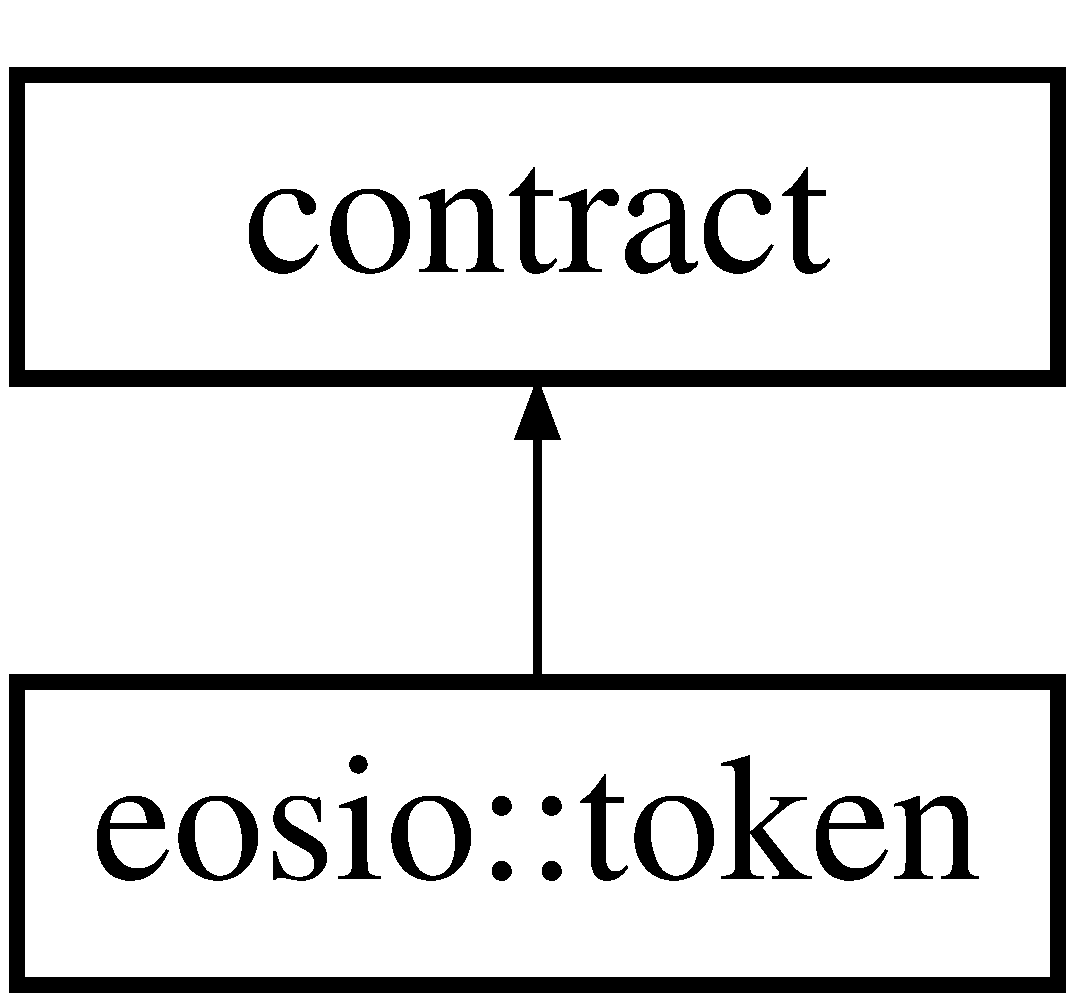
\includegraphics[height=2.000000cm]{classeosio_1_1token}
\end{center}
\end{figure}
\subsection*{Public Types}
\begin{DoxyCompactItemize}
\item 
\mbox{\Hypertarget{classeosio_1_1token_ab6f5f8e8c550b3ae9492fcde3f04458a}\label{classeosio_1_1token_ab6f5f8e8c550b3ae9492fcde3f04458a}} 
using {\bfseries create\+\_\+action} = eosio\+::action\+\_\+wrapper$<$\char`\"{}create\char`\"{}\+\_\+n, \&token\+::create $>$
\item 
\mbox{\Hypertarget{classeosio_1_1token_a0a264928ea4b4c3056884cc95c9bea49}\label{classeosio_1_1token_a0a264928ea4b4c3056884cc95c9bea49}} 
using {\bfseries issue\+\_\+action} = eosio\+::action\+\_\+wrapper$<$\char`\"{}issue\char`\"{}\+\_\+n, \&token\+::issue $>$
\item 
\mbox{\Hypertarget{classeosio_1_1token_adebe02a32df2bf3ca7f27eec264b32c4}\label{classeosio_1_1token_adebe02a32df2bf3ca7f27eec264b32c4}} 
using {\bfseries retire\+\_\+action} = eosio\+::action\+\_\+wrapper$<$\char`\"{}retire\char`\"{}\+\_\+n, \&token\+::retire $>$
\item 
\mbox{\Hypertarget{classeosio_1_1token_a48e0c826f1e416bf99439b0b7e637a29}\label{classeosio_1_1token_a48e0c826f1e416bf99439b0b7e637a29}} 
using {\bfseries transfer\+\_\+action} = eosio\+::action\+\_\+wrapper$<$\char`\"{}transfer\char`\"{}\+\_\+n, \&token\+::transfer $>$
\item 
\mbox{\Hypertarget{classeosio_1_1token_aee1aaa798e4d4a973b40a5a4b95d2a21}\label{classeosio_1_1token_aee1aaa798e4d4a973b40a5a4b95d2a21}} 
using {\bfseries open\+\_\+action} = eosio\+::action\+\_\+wrapper$<$\char`\"{}open\char`\"{}\+\_\+n, \&token\+::open $>$
\item 
\mbox{\Hypertarget{classeosio_1_1token_a3e49a7888cde765dfe8f4966b3067036}\label{classeosio_1_1token_a3e49a7888cde765dfe8f4966b3067036}} 
using {\bfseries close\+\_\+action} = eosio\+::action\+\_\+wrapper$<$\char`\"{}close\char`\"{}\+\_\+n, \&token\+::close $>$
\end{DoxyCompactItemize}
\subsection*{Public Member Functions}
\begin{DoxyCompactItemize}
\item 
\mbox{\Hypertarget{classeosio_1_1token_a398d3ab0784aa52d314ff47666c51701}\label{classeosio_1_1token_a398d3ab0784aa52d314ff47666c51701}} 
void {\bfseries create} (name issuer, asset maximum\+\_\+supply)
\item 
\mbox{\Hypertarget{classeosio_1_1token_a7dc16dac15ffa8313424676fc02c7015}\label{classeosio_1_1token_a7dc16dac15ffa8313424676fc02c7015}} 
void {\bfseries issue} (name to, asset quantity, string memo)
\item 
\mbox{\Hypertarget{classeosio_1_1token_a29c839dfaad1b3c46c2c3ababf232359}\label{classeosio_1_1token_a29c839dfaad1b3c46c2c3ababf232359}} 
void {\bfseries retire} (asset quantity, string memo)
\item 
\mbox{\Hypertarget{classeosio_1_1token_a47e89b1fb0cf66946528bdebd9c786d9}\label{classeosio_1_1token_a47e89b1fb0cf66946528bdebd9c786d9}} 
void {\bfseries transfer} (name from, name to, asset quantity, string memo)
\item 
\mbox{\Hypertarget{classeosio_1_1token_a119743fdb70ea5f9dc1fea2c7774ed2d}\label{classeosio_1_1token_a119743fdb70ea5f9dc1fea2c7774ed2d}} 
void {\bfseries open} (name owner, const symbol \&symbol, name ram\+\_\+payer)
\item 
\mbox{\Hypertarget{classeosio_1_1token_a35f91e5e77635f0dfadc0eea93ec9da7}\label{classeosio_1_1token_a35f91e5e77635f0dfadc0eea93ec9da7}} 
void {\bfseries close} (name owner, const symbol \&symbol)
\end{DoxyCompactItemize}
\subsection*{Static Public Member Functions}
\begin{DoxyCompactItemize}
\item 
\mbox{\Hypertarget{classeosio_1_1token_a1fb6c9a84871da4fb2f6023de5351dcf}\label{classeosio_1_1token_a1fb6c9a84871da4fb2f6023de5351dcf}} 
static asset {\bfseries get\+\_\+supply} (name token\+\_\+contract\+\_\+account, symbol\+\_\+code sym\+\_\+code)
\item 
\mbox{\Hypertarget{classeosio_1_1token_a10fdccf5b89beaea3ba8fa5e300675bc}\label{classeosio_1_1token_a10fdccf5b89beaea3ba8fa5e300675bc}} 
static asset {\bfseries get\+\_\+max\+\_\+supply} (name token\+\_\+contract\+\_\+account, symbol\+\_\+code sym\+\_\+code)
\item 
\mbox{\Hypertarget{classeosio_1_1token_a3d5912b5b8a3a76d91b9fae94695e58f}\label{classeosio_1_1token_a3d5912b5b8a3a76d91b9fae94695e58f}} 
static asset {\bfseries get\+\_\+balance} (name token\+\_\+contract\+\_\+account, name owner, symbol\+\_\+code sym\+\_\+code)
\end{DoxyCompactItemize}


\subsection{Detailed Description}
Класс взаимодействия с жетонами операционной системы. 

The documentation for this class was generated from the following file\+:\begin{DoxyCompactItemize}
\item 
include/eosio.\+token.\+hpp\end{DoxyCompactItemize}

\hypertarget{structeosio_1_1token_1_1transfer__args}{}\section{eosio\+:\+:token\+:\+:transfer\+\_\+args Struct Reference}
\label{structeosio_1_1token_1_1transfer__args}\index{eosio\+::token\+::transfer\+\_\+args@{eosio\+::token\+::transfer\+\_\+args}}
\subsection*{Public Attributes}
\begin{DoxyCompactItemize}
\item 
\mbox{\Hypertarget{structeosio_1_1token_1_1transfer__args_a7c88c1ade6cb2cdd431977e0c3b3668e}\label{structeosio_1_1token_1_1transfer__args_a7c88c1ade6cb2cdd431977e0c3b3668e}} 
account\+\_\+name {\bfseries from}
\item 
\mbox{\Hypertarget{structeosio_1_1token_1_1transfer__args_a8d0efe51d87131b936f336b82f2683f4}\label{structeosio_1_1token_1_1transfer__args_a8d0efe51d87131b936f336b82f2683f4}} 
account\+\_\+name {\bfseries to}
\item 
\mbox{\Hypertarget{structeosio_1_1token_1_1transfer__args_a8739988eae06a643dbbb62bd4ea4556a}\label{structeosio_1_1token_1_1transfer__args_a8739988eae06a643dbbb62bd4ea4556a}} 
asset {\bfseries quantity}
\item 
\mbox{\Hypertarget{structeosio_1_1token_1_1transfer__args_a93525854f40c4d7aaa9f18ab3404930e}\label{structeosio_1_1token_1_1transfer__args_a93525854f40c4d7aaa9f18ab3404930e}} 
string {\bfseries memo}
\end{DoxyCompactItemize}


The documentation for this struct was generated from the following file\+:\begin{DoxyCompactItemize}
\item 
\mbox{\hyperlink{eosio_8token_8hpp}{eosio.\+token.\+hpp}}\end{DoxyCompactItemize}

\hypertarget{structeosio_1_1tsks}{}\section{eosio\+:\+:tsks Struct Reference}
\label{structeosio_1_1tsks}\index{eosio\+::tsks@{eosio\+::tsks}}
\subsection*{Public Member Functions}
\begin{DoxyCompactItemize}
\item 
\mbox{\Hypertarget{structeosio_1_1tsks_a36b4b16563aee29ef3af8af63a8aec1f}\label{structeosio_1_1tsks_a36b4b16563aee29ef3af8af63a8aec1f}} 
void {\bfseries settask\+\_\+action} (const \mbox{\hyperlink{structeosio_1_1settask}{settask}} \&op)
\item 
\mbox{\Hypertarget{structeosio_1_1tsks_af5c40f1675c91ade36ac34d105e6a8e3}\label{structeosio_1_1tsks_af5c40f1675c91ade36ac34d105e6a8e3}} 
void {\bfseries fundtask\+\_\+action} (const \mbox{\hyperlink{structeosio_1_1fundtask}{fundtask}} \&op)
\item 
\mbox{\Hypertarget{structeosio_1_1tsks_ad6ccc424854393d8871818961bca6787}\label{structeosio_1_1tsks_ad6ccc424854393d8871818961bca6787}} 
void {\bfseries tactivate\+\_\+action} (const \mbox{\hyperlink{structeosio_1_1tactivate}{tactivate}} \&op)
\item 
\mbox{\Hypertarget{structeosio_1_1tsks_aca63fc18e2ceea00bdc6e438ce751e28}\label{structeosio_1_1tsks_aca63fc18e2ceea00bdc6e438ce751e28}} 
void {\bfseries tdeactivate\+\_\+action} (const \mbox{\hyperlink{structeosio_1_1tdeactivate}{tdeactivate}} \&op)
\item 
\mbox{\Hypertarget{structeosio_1_1tsks_a83745c040c6a12dddcd9063865b81caa}\label{structeosio_1_1tsks_a83745c040c6a12dddcd9063865b81caa}} 
void {\bfseries setreport\+\_\+action} (const \mbox{\hyperlink{structeosio_1_1setreport}{setreport}} \&op)
\item 
\mbox{\Hypertarget{structeosio_1_1tsks_aadd8eeb3a74a671e2fa30e38ba73baee}\label{structeosio_1_1tsks_aadd8eeb3a74a671e2fa30e38ba73baee}} 
void {\bfseries editreport\+\_\+action} (const \mbox{\hyperlink{structeosio_1_1editreport}{editreport}} \&op)
\item 
\mbox{\Hypertarget{structeosio_1_1tsks_a1ec801c9cab2c613ba6e4a8e005e3c0c}\label{structeosio_1_1tsks_a1ec801c9cab2c613ba6e4a8e005e3c0c}} 
void {\bfseries approver\+\_\+action} (const \mbox{\hyperlink{structeosio_1_1approver}{approver}} \&op)
\item 
\mbox{\Hypertarget{structeosio_1_1tsks_a13940dec55cf59369111aa1a1ac9b2e9}\label{structeosio_1_1tsks_a13940dec55cf59369111aa1a1ac9b2e9}} 
void {\bfseries disapprover\+\_\+action} (const \mbox{\hyperlink{structeosio_1_1disapprover}{disapprover}} \&op)
\end{DoxyCompactItemize}


The documentation for this struct was generated from the following file\+:\begin{DoxyCompactItemize}
\item 
tasks.\+cpp\end{DoxyCompactItemize}

\hypertarget{structeosio_1_1undelshares}{}\section{eosio\+:\+:undelshares Struct Reference}
\label{structeosio_1_1undelshares}\index{eosio\+::undelshares@{eosio\+::undelshares}}
\subsection*{Public Attributes}
\begin{DoxyCompactItemize}
\item 
\mbox{\Hypertarget{structeosio_1_1undelshares_ace166bd54b1b4193d449b6d0004fd8d5}\label{structeosio_1_1undelshares_ace166bd54b1b4193d449b6d0004fd8d5}} 
account\+\_\+name {\bfseries from}
\item 
\mbox{\Hypertarget{structeosio_1_1undelshares_ab59b50fe824d47e0e8ca1d0dcda1b977}\label{structeosio_1_1undelshares_ab59b50fe824d47e0e8ca1d0dcda1b977}} 
account\+\_\+name {\bfseries reciever}
\item 
\mbox{\Hypertarget{structeosio_1_1undelshares_a24dc07b9c9d728a959db8b3d904a5e7e}\label{structeosio_1_1undelshares_a24dc07b9c9d728a959db8b3d904a5e7e}} 
account\+\_\+name {\bfseries host}
\item 
\mbox{\Hypertarget{structeosio_1_1undelshares_a5c139b4398ce7ec6b32f1dff13563082}\label{structeosio_1_1undelshares_a5c139b4398ce7ec6b32f1dff13563082}} 
uint64\+\_\+t {\bfseries shares}
\end{DoxyCompactItemize}


The documentation for this struct was generated from the following file\+:\begin{DoxyCompactItemize}
\item 
shares.\+hpp\end{DoxyCompactItemize}

\hypertarget{structeosio_1_1upgrade}{}\section{eosio\+:\+:upgrade Struct Reference}
\label{structeosio_1_1upgrade}\index{eosio\+::upgrade@{eosio\+::upgrade}}
\subsection*{Public Attributes}
\begin{DoxyCompactItemize}
\item 
\mbox{\Hypertarget{structeosio_1_1upgrade_aca34ed7f60c0082ccdd9281ab9df5e05}\label{structeosio_1_1upgrade_aca34ed7f60c0082ccdd9281ab9df5e05}} 
account\+\_\+name {\bfseries username}
\item 
\mbox{\Hypertarget{structeosio_1_1upgrade_a1fdfe36f9b23708bda09a1e2cf4ac5a9}\label{structeosio_1_1upgrade_a1fdfe36f9b23708bda09a1e2cf4ac5a9}} 
std\+::string {\bfseries title}
\item 
\mbox{\Hypertarget{structeosio_1_1upgrade_ab4d5ffff08774557a95aa7c6e23723e5}\label{structeosio_1_1upgrade_ab4d5ffff08774557a95aa7c6e23723e5}} 
std\+::string {\bfseries purpose}
\item 
\mbox{\Hypertarget{structeosio_1_1upgrade_a69a8b76a33fa3619b2114885cd16115c}\label{structeosio_1_1upgrade_a69a8b76a33fa3619b2114885cd16115c}} 
uint64\+\_\+t {\bfseries total\+\_\+shares}
\item 
\mbox{\Hypertarget{structeosio_1_1upgrade_a5131e0eaa3eabcd228519cef32c39075}\label{structeosio_1_1upgrade_a5131e0eaa3eabcd228519cef32c39075}} 
eosio\+::asset {\bfseries quote\+\_\+amount}
\item 
\mbox{\Hypertarget{structeosio_1_1upgrade_ae40e9f70ed8d453b4892960859cb6864}\label{structeosio_1_1upgrade_ae40e9f70ed8d453b4892960859cb6864}} 
eosio\+::asset {\bfseries root\+\_\+token}
\item 
\mbox{\Hypertarget{structeosio_1_1upgrade_a5d79a63e14844937dab45237e4f0fcd9}\label{structeosio_1_1upgrade_a5d79a63e14844937dab45237e4f0fcd9}} 
account\+\_\+name {\bfseries root\+\_\+token\+\_\+contract}
\item 
\mbox{\Hypertarget{structeosio_1_1upgrade_ab286ffcaa3a70d42699bb0b869b2a458}\label{structeosio_1_1upgrade_ab286ffcaa3a70d42699bb0b869b2a458}} 
uint64\+\_\+t {\bfseries consensus\+\_\+percent}
\item 
\mbox{\Hypertarget{structeosio_1_1upgrade_ae5f0ac6cc80361aa1f7309adbcfce9d8}\label{structeosio_1_1upgrade_ae5f0ac6cc80361aa1f7309adbcfce9d8}} 
uint64\+\_\+t {\bfseries referral\+\_\+percent}
\item 
\mbox{\Hypertarget{structeosio_1_1upgrade_a8086d7110af3723c2ef61cef732dc0f2}\label{structeosio_1_1upgrade_a8086d7110af3723c2ef61cef732dc0f2}} 
uint64\+\_\+t {\bfseries dacs\+\_\+percent}
\item 
\mbox{\Hypertarget{structeosio_1_1upgrade_ad72c7d67ce35690581741b4ab1296155}\label{structeosio_1_1upgrade_ad72c7d67ce35690581741b4ab1296155}} 
std\+::vector$<$ uint64\+\_\+t $>$ {\bfseries levels}
\item 
\mbox{\Hypertarget{structeosio_1_1upgrade_af5dc369ac7f5a1025488820aa8272bc3}\label{structeosio_1_1upgrade_af5dc369ac7f5a1025488820aa8272bc3}} 
std\+::string {\bfseries meta}
\end{DoxyCompactItemize}


The documentation for this struct was generated from the following file\+:\begin{DoxyCompactItemize}
\item 
hosts.\+hpp\end{DoxyCompactItemize}

\hypertarget{structeosio_1_1usbadges}{}\section{eosio\+:\+:usbadges Struct Reference}
\label{structeosio_1_1usbadges}\index{eosio\+::usbadges@{eosio\+::usbadges}}
\subsection*{Public Member Functions}
\begin{DoxyCompactItemize}
\item 
\mbox{\Hypertarget{structeosio_1_1usbadges_a82542c6ea2cacdc6249264787e6086ec}\label{structeosio_1_1usbadges_a82542c6ea2cacdc6249264787e6086ec}} 
uint64\+\_\+t {\bfseries primary\+\_\+key} () const
\item 
\mbox{\Hypertarget{structeosio_1_1usbadges_ab26c4b6cc771bfe7bc0f6b9a242c1e57}\label{structeosio_1_1usbadges_ab26c4b6cc771bfe7bc0f6b9a242c1e57}} 
uint64\+\_\+t {\bfseries host\+\_\+key} () const
\end{DoxyCompactItemize}
\subsection*{Public Attributes}
\begin{DoxyCompactItemize}
\item 
\mbox{\Hypertarget{structeosio_1_1usbadges_a1c3f9c15745c491f581dfe220c8b0836}\label{structeosio_1_1usbadges_a1c3f9c15745c491f581dfe220c8b0836}} 
uint64\+\_\+t {\bfseries id}
\item 
\mbox{\Hypertarget{structeosio_1_1usbadges_a38bac4b28a51306b00fca9a987f7b8ed}\label{structeosio_1_1usbadges_a38bac4b28a51306b00fca9a987f7b8ed}} 
account\+\_\+name {\bfseries host}
\item 
\mbox{\Hypertarget{structeosio_1_1usbadges_aaad08f86c6d530851266d574bea00bb0}\label{structeosio_1_1usbadges_aaad08f86c6d530851266d574bea00bb0}} 
uint64\+\_\+t {\bfseries badge\+\_\+type}
\item 
\mbox{\Hypertarget{structeosio_1_1usbadges_a4473d8550fcc7dcb0b4ce36cf50f9780}\label{structeosio_1_1usbadges_a4473d8550fcc7dcb0b4ce36cf50f9780}} 
eosio\+::string {\bfseries caption}
\item 
\mbox{\Hypertarget{structeosio_1_1usbadges_ade0c25ea48fd7d4a2404d305d0c44138}\label{structeosio_1_1usbadges_ade0c25ea48fd7d4a2404d305d0c44138}} 
eosio\+::string {\bfseries description}
\item 
\mbox{\Hypertarget{structeosio_1_1usbadges_a469996cf77d33b5fb5b6befbe27e9446}\label{structeosio_1_1usbadges_a469996cf77d33b5fb5b6befbe27e9446}} 
eosio\+::string {\bfseries iurl}
\item 
\mbox{\Hypertarget{structeosio_1_1usbadges_a33f9796364181ec39ed3a931f3aa694a}\label{structeosio_1_1usbadges_a33f9796364181ec39ed3a931f3aa694a}} 
eosio\+::string {\bfseries comment}
\item 
\mbox{\Hypertarget{structeosio_1_1usbadges_a9149d3a9abaf9ea7e10d9937033cb79d}\label{structeosio_1_1usbadges_a9149d3a9abaf9ea7e10d9937033cb79d}} 
eosio\+::time\+\_\+point\+\_\+sec {\bfseries recieved\+\_\+at}
\item 
\mbox{\Hypertarget{structeosio_1_1usbadges_a86466d8cb7eac5bd731a377b5147fe1b}\label{structeosio_1_1usbadges_a86466d8cb7eac5bd731a377b5147fe1b}} 
bool {\bfseries backed} = false
\item 
\mbox{\Hypertarget{structeosio_1_1usbadges_a280fd395d00e11639d2c8cd56ca9475d}\label{structeosio_1_1usbadges_a280fd395d00e11639d2c8cd56ca9475d}} 
eosio\+::string {\bfseries backreason}
\end{DoxyCompactItemize}


The documentation for this struct was generated from the following file\+:\begin{DoxyCompactItemize}
\item 
badges.\+hpp\end{DoxyCompactItemize}

\hypertarget{structeosio_1_1userdatacnts}{}\section{eosio\+:\+:userdatacnts Struct Reference}
\label{structeosio_1_1userdatacnts}\index{eosio\+::userdatacnts@{eosio\+::userdatacnts}}
\subsection*{Public Member Functions}
\begin{DoxyCompactItemize}
\item 
\mbox{\Hypertarget{structeosio_1_1userdatacnts_a4fc8a474ce6c223ee99cb983248f9e38}\label{structeosio_1_1userdatacnts_a4fc8a474ce6c223ee99cb983248f9e38}} 
uint64\+\_\+t {\bfseries primary\+\_\+key} () const
\end{DoxyCompactItemize}
\subsection*{Public Attributes}
\begin{DoxyCompactItemize}
\item 
\mbox{\Hypertarget{structeosio_1_1userdatacnts_a2ac06404838ec7df93ceec0234c670ff}\label{structeosio_1_1userdatacnts_a2ac06404838ec7df93ceec0234c670ff}} 
account\+\_\+name {\bfseries username}
\item 
\mbox{\Hypertarget{structeosio_1_1userdatacnts_a3a83d18a66b2b09413fc781a6cf6bf58}\label{structeosio_1_1userdatacnts_a3a83d18a66b2b09413fc781a6cf6bf58}} 
uint64\+\_\+t {\bfseries total\+\_\+sales} = 0
\item 
\mbox{\Hypertarget{structeosio_1_1userdatacnts_a743abf1afd346de99d8ceb8c86f78e54}\label{structeosio_1_1userdatacnts_a743abf1afd346de99d8ceb8c86f78e54}} 
uint64\+\_\+t {\bfseries total\+\_\+buys} = 0
\item 
\mbox{\Hypertarget{structeosio_1_1userdatacnts_a45d2a348699d0d67fabbf60cf9d2e3b5}\label{structeosio_1_1userdatacnts_a45d2a348699d0d67fabbf60cf9d2e3b5}} 
uint64\+\_\+t {\bfseries total\+\_\+disputes} = 0
\item 
\mbox{\Hypertarget{structeosio_1_1userdatacnts_a252cda88be8dfc344889a9868fdeb744}\label{structeosio_1_1userdatacnts_a252cda88be8dfc344889a9868fdeb744}} 
uint64\+\_\+t {\bfseries p\+\_\+disputes} = 0
\item 
\mbox{\Hypertarget{structeosio_1_1userdatacnts_a7d2ecd93e666b68ad4dca92c2ab703fd}\label{structeosio_1_1userdatacnts_a7d2ecd93e666b68ad4dca92c2ab703fd}} 
uint64\+\_\+t {\bfseries n\+\_\+disputes} = 0
\end{DoxyCompactItemize}


The documentation for this struct was generated from the following file\+:\begin{DoxyCompactItemize}
\item 
ipfs.\+hpp\end{DoxyCompactItemize}

\hypertarget{structeosio_1_1users}{}\section{eosio\+:\+:users Struct Reference}
\label{structeosio_1_1users}\index{eosio\+::users@{eosio\+::users}}
\subsection*{Public Member Functions}
\begin{DoxyCompactItemize}
\item 
\mbox{\Hypertarget{structeosio_1_1users_a47aa2a1fb7e34ca0b5bc1a16df09d4be}\label{structeosio_1_1users_a47aa2a1fb7e34ca0b5bc1a16df09d4be}} 
uint64\+\_\+t {\bfseries primary\+\_\+key} () const
\item 
\mbox{\Hypertarget{structeosio_1_1users_a32651e54b2b3b4eb456d794a7a5c9857}\label{structeosio_1_1users_a32651e54b2b3b4eb456d794a7a5c9857}} 
uint64\+\_\+t {\bfseries byreferer} () const
\end{DoxyCompactItemize}
\subsection*{Public Attributes}
\begin{DoxyCompactItemize}
\item 
\mbox{\Hypertarget{structeosio_1_1users_a44c509f50d397d7d6c73116a18262a52}\label{structeosio_1_1users_a44c509f50d397d7d6c73116a18262a52}} 
eosio\+::name {\bfseries username}
\item 
\mbox{\Hypertarget{structeosio_1_1users_afab2bcf1c4687bc9a1566c63a2929fde}\label{structeosio_1_1users_afab2bcf1c4687bc9a1566c63a2929fde}} 
eosio\+::name {\bfseries referer}
\item 
\mbox{\Hypertarget{structeosio_1_1users_a5e887dd79303688eecab2f3c30377b28}\label{structeosio_1_1users_a5e887dd79303688eecab2f3c30377b28}} 
uint64\+\_\+t {\bfseries id}
\item 
\mbox{\Hypertarget{structeosio_1_1users_abd1a3bad3b68b2d470f21b4431c58d1e}\label{structeosio_1_1users_abd1a3bad3b68b2d470f21b4431c58d1e}} 
bool {\bfseries is\+\_\+host} = false
\item 
\mbox{\Hypertarget{structeosio_1_1users_a75ad43ee45326207c97029d337d3b1fc}\label{structeosio_1_1users_a75ad43ee45326207c97029d337d3b1fc}} 
std\+::string {\bfseries meta}
\end{DoxyCompactItemize}


The documentation for this struct was generated from the following file\+:\begin{DoxyCompactItemize}
\item 
include/core.\+hpp\end{DoxyCompactItemize}

\hypertarget{structeosio_1_1vesting}{}\section{eosio\+:\+:vesting Struct Reference}
\label{structeosio_1_1vesting}\index{eosio\+::vesting@{eosio\+::vesting}}
\subsection*{Public Member Functions}
\begin{DoxyCompactItemize}
\item 
\mbox{\Hypertarget{structeosio_1_1vesting_a3c093ab61055f1a0c3a667ba9c2855ab}\label{structeosio_1_1vesting_a3c093ab61055f1a0c3a667ba9c2855ab}} 
uint64\+\_\+t {\bfseries primary\+\_\+key} () const
\end{DoxyCompactItemize}
\subsection*{Public Attributes}
\begin{DoxyCompactItemize}
\item 
\mbox{\Hypertarget{structeosio_1_1vesting_ae98570990c942ebdcb171d344a8db7f8}\label{structeosio_1_1vesting_ae98570990c942ebdcb171d344a8db7f8}} 
uint64\+\_\+t {\bfseries id}
\item 
\mbox{\Hypertarget{structeosio_1_1vesting_ae8b54fe4dc52efe7739788ec0cfd1346}\label{structeosio_1_1vesting_ae8b54fe4dc52efe7739788ec0cfd1346}} 
account\+\_\+name {\bfseries owner}
\item 
\mbox{\Hypertarget{structeosio_1_1vesting_ab3907ffc6e5e062cb6a1496b6db0679b}\label{structeosio_1_1vesting_ab3907ffc6e5e062cb6a1496b6db0679b}} 
eosio\+::time\+\_\+point\+\_\+sec {\bfseries startat}
\item 
\mbox{\Hypertarget{structeosio_1_1vesting_a6c24c93faf099c7378a3985b9ea0eb2c}\label{structeosio_1_1vesting_a6c24c93faf099c7378a3985b9ea0eb2c}} 
uint64\+\_\+t {\bfseries duration}
\item 
\mbox{\Hypertarget{structeosio_1_1vesting_ae3667ebbeb0a29faceb2e2833271d5ec}\label{structeosio_1_1vesting_ae3667ebbeb0a29faceb2e2833271d5ec}} 
eosio\+::asset {\bfseries amount}
\item 
\mbox{\Hypertarget{structeosio_1_1vesting_a589b29d72d033f44a6b18181613fc618}\label{structeosio_1_1vesting_a589b29d72d033f44a6b18181613fc618}} 
eosio\+::asset {\bfseries available}
\item 
\mbox{\Hypertarget{structeosio_1_1vesting_a2ddc10868b15ef3a150d4d19591fe232}\label{structeosio_1_1vesting_a2ddc10868b15ef3a150d4d19591fe232}} 
eosio\+::asset {\bfseries withdrawed}
\end{DoxyCompactItemize}


The documentation for this struct was generated from the following file\+:\begin{DoxyCompactItemize}
\item 
shares.\+hpp\end{DoxyCompactItemize}

\hypertarget{structeosio_1_1vote}{}\section{eosio\+:\+:vote Struct Reference}
\label{structeosio_1_1vote}\index{eosio\+::vote@{eosio\+::vote}}
\subsection*{Public Attributes}
\begin{DoxyCompactItemize}
\item 
\mbox{\Hypertarget{structeosio_1_1vote_a6bdea781cbcc39dde9d7fc46a548968c}\label{structeosio_1_1vote_a6bdea781cbcc39dde9d7fc46a548968c}} 
account\+\_\+name {\bfseries voter}
\item 
\mbox{\Hypertarget{structeosio_1_1vote_ac683ded160c11a294e1720fda5a62b03}\label{structeosio_1_1vote_ac683ded160c11a294e1720fda5a62b03}} 
account\+\_\+name {\bfseries host}
\item 
\mbox{\Hypertarget{structeosio_1_1vote_ac17320874168bcbfdb4db58dd6e3ba82}\label{structeosio_1_1vote_ac17320874168bcbfdb4db58dd6e3ba82}} 
uint64\+\_\+t {\bfseries goal\+\_\+id}
\item 
\mbox{\Hypertarget{structeosio_1_1vote_a28b87c515530fa005cbbcdd3d868b683}\label{structeosio_1_1vote_a28b87c515530fa005cbbcdd3d868b683}} 
bool {\bfseries up}
\end{DoxyCompactItemize}


The documentation for this struct was generated from the following file\+:\begin{DoxyCompactItemize}
\item 
voting.\+hpp\end{DoxyCompactItemize}

\hypertarget{structeosio_1_1votes}{}\section{eosio\+:\+:votes Struct Reference}
\label{structeosio_1_1votes}\index{eosio\+::votes@{eosio\+::votes}}
\subsection*{Public Member Functions}
\begin{DoxyCompactItemize}
\item 
\mbox{\Hypertarget{structeosio_1_1votes_ae77211beb2cabd6b8cf5bf1fd48ab1ad}\label{structeosio_1_1votes_ae77211beb2cabd6b8cf5bf1fd48ab1ad}} 
uint64\+\_\+t {\bfseries primary\+\_\+key} () const
\item 
\mbox{\Hypertarget{structeosio_1_1votes_aa8382302b8f3db0de182af73b7a7d4c6}\label{structeosio_1_1votes_aa8382302b8f3db0de182af73b7a7d4c6}} 
account\+\_\+name {\bfseries by\+\_\+host} () const
\item 
\mbox{\Hypertarget{structeosio_1_1votes_a8db493f978427a54f36d83b29c188a84}\label{structeosio_1_1votes_a8db493f978427a54f36d83b29c188a84}} 
uint128\+\_\+t {\bfseries id\+\_\+with\+\_\+host} () const
\end{DoxyCompactItemize}
\subsection*{Public Attributes}
\begin{DoxyCompactItemize}
\item 
\mbox{\Hypertarget{structeosio_1_1votes_a3f9015b0bc3aa4d49f89770b1b123108}\label{structeosio_1_1votes_a3f9015b0bc3aa4d49f89770b1b123108}} 
uint64\+\_\+t {\bfseries id}
\item 
\mbox{\Hypertarget{structeosio_1_1votes_a429610e81636e333de9272c08b58e630}\label{structeosio_1_1votes_a429610e81636e333de9272c08b58e630}} 
uint64\+\_\+t {\bfseries goal\+\_\+id}
\item 
\mbox{\Hypertarget{structeosio_1_1votes_a68474af393100808fb5b4c314df7a0d9}\label{structeosio_1_1votes_a68474af393100808fb5b4c314df7a0d9}} 
account\+\_\+name {\bfseries host}
\item 
\mbox{\Hypertarget{structeosio_1_1votes_a7342aab3f84b616a2a5a81bf629648f9}\label{structeosio_1_1votes_a7342aab3f84b616a2a5a81bf629648f9}} 
int64\+\_\+t {\bfseries power}
\end{DoxyCompactItemize}


The documentation for this struct was generated from the following file\+:\begin{DoxyCompactItemize}
\item 
voting.\+hpp\end{DoxyCompactItemize}

\hypertarget{structeosio_1_1voting}{}\section{eosio\+:\+:voting Struct Reference}
\label{structeosio_1_1voting}\index{eosio\+::voting@{eosio\+::voting}}
\subsection*{Public Member Functions}
\begin{DoxyCompactItemize}
\item 
\mbox{\Hypertarget{structeosio_1_1voting_aeee24d2bf2742584f5a3e764cd856bfb}\label{structeosio_1_1voting_aeee24d2bf2742584f5a3e764cd856bfb}} 
void {\bfseries clear\+\_\+old\+\_\+votes\+\_\+action} (account\+\_\+name voter, account\+\_\+name host)
\item 
\mbox{\Hypertarget{structeosio_1_1voting_a3c048fa20881ff15662ddc2380c3b426}\label{structeosio_1_1voting_a3c048fa20881ff15662ddc2380c3b426}} 
uint64\+\_\+t {\bfseries count\+\_\+votes} (account\+\_\+name voter, account\+\_\+name host)
\item 
\mbox{\Hypertarget{structeosio_1_1voting_a8eb127d952c2f5b5705c467617fef457}\label{structeosio_1_1voting_a8eb127d952c2f5b5705c467617fef457}} 
void {\bfseries vote\+\_\+action} (const \mbox{\hyperlink{structeosio_1_1vote}{vote}} \&op)
\end{DoxyCompactItemize}


The documentation for this struct was generated from the following file\+:\begin{DoxyCompactItemize}
\item 
voting.\+cpp\end{DoxyCompactItemize}

\hypertarget{structeosio_1_1withdraw}{}\section{eosio\+:\+:withdraw Struct Reference}
\label{structeosio_1_1withdraw}\index{eosio\+::withdraw@{eosio\+::withdraw}}
\subsection*{Public Attributes}
\begin{DoxyCompactItemize}
\item 
\mbox{\Hypertarget{structeosio_1_1withdraw_a27762de6952a2d466c2a888dbf7e356a}\label{structeosio_1_1withdraw_a27762de6952a2d466c2a888dbf7e356a}} 
account\+\_\+name {\bfseries username}
\item 
\mbox{\Hypertarget{structeosio_1_1withdraw_a1da5d9e772825b4db8bbf0513e2ae16f}\label{structeosio_1_1withdraw_a1da5d9e772825b4db8bbf0513e2ae16f}} 
account\+\_\+name {\bfseries host}
\item 
\mbox{\Hypertarget{structeosio_1_1withdraw_aa47fcc12665cea0c7afdb3e41aeb5a18}\label{structeosio_1_1withdraw_aa47fcc12665cea0c7afdb3e41aeb5a18}} 
uint64\+\_\+t {\bfseries balance\+\_\+id}
\end{DoxyCompactItemize}


The documentation for this struct was generated from the following file\+:\begin{DoxyCompactItemize}
\item 
protocol.\+hpp\end{DoxyCompactItemize}

\hypertarget{structeosio_1_1withdrawsh}{}\section{eosio\+:\+:withdrawsh Struct Reference}
\label{structeosio_1_1withdrawsh}\index{eosio\+::withdrawsh@{eosio\+::withdrawsh}}
\subsection*{Public Attributes}
\begin{DoxyCompactItemize}
\item 
\mbox{\Hypertarget{structeosio_1_1withdrawsh_ac87016a69b003e7ae98b6260f9d069a5}\label{structeosio_1_1withdrawsh_ac87016a69b003e7ae98b6260f9d069a5}} 
account\+\_\+name {\bfseries owner}
\item 
\mbox{\Hypertarget{structeosio_1_1withdrawsh_a7bfb70bfb56d4ac26c7361d8e8478c97}\label{structeosio_1_1withdrawsh_a7bfb70bfb56d4ac26c7361d8e8478c97}} 
uint64\+\_\+t {\bfseries id}
\end{DoxyCompactItemize}


The documentation for this struct was generated from the following file\+:\begin{DoxyCompactItemize}
\item 
shares.\+hpp\end{DoxyCompactItemize}

\chapter{File Documentation}
\hypertarget{eosio_8token_8hpp}{}\section{eosio.\+token.\+hpp File Reference}
\label{eosio_8token_8hpp}\index{eosio.\+token.\+hpp@{eosio.\+token.\+hpp}}
{\ttfamily \#include $<$eosiolib/asset.\+hpp$>$}\newline
{\ttfamily \#include $<$eosiolib/eosio.\+hpp$>$}\newline
{\ttfamily \#include $<$string$>$}\newline
\subsection*{Classes}
\begin{DoxyCompactItemize}
\item 
class \mbox{\hyperlink{classeosio_1_1token}{eosio\+::token}}
\item 
struct \mbox{\hyperlink{structeosio_1_1token_1_1transfer__args}{eosio\+::token\+::transfer\+\_\+args}}
\end{DoxyCompactItemize}


\subsection{Detailed Description}
\begin{DoxyCopyright}{Copyright}
defined in eos/\+L\+I\+C\+E\+N\+S\+E.\+txt 
\end{DoxyCopyright}

%--- End generated contents ---

% Index
\backmatter
\newpage
\phantomsection
\clearemptydoublepage
\addcontentsline{toc}{chapter}{Index}
\printindex

\end{document}
